\documentclass[a4paper,10pt]{article}

% --- Pacchetti minimi ---
\usepackage[utf8]{inputenc}
\usepackage[T1]{fontenc}
\usepackage[italian]{babel}
\usepackage{amsmath}
\usepackage{array}
\usepackage{adjustbox}
\usepackage{geometry}
\usepackage[table]{xcolor} 
\definecolor{myblue}{HTML}{139FE9}
\geometry{margin=1.5cm}
\usepackage{footnote}
% Pacchetti per Layout e Formattazione 
\usepackage{fancyhdr} 
\usepackage{float} 
% Pacchetti Grafici e Diagrammi 
\usepackage{graphicx} 
\usepackage{tikz} 
\usepackage{tikz-3dplot} 
\usetikzlibrary{angles,quotes,arrows.meta, positioning} 
\usepackage{pgfplots} 
\pgfplotsset{compat=1.18} % Pacchetti Matematici 
\usepackage{amsmath, amssymb, amsthm} 


\usepackage{siunitx} 
\usepackage{eurosym} 
% --- Spaziatura tabella ---
\setlength{\extrarowheight}{2pt}

% --- Solo i comandi necessari (Note/Descrizioni) ---
\newcommand{\roaDesc}{Misura la redditività complessiva dell’impresa rispetto al totale delle attività. Utile per confronti tra aziende con strutture finanziarie diverse, perché parte dall’EBIT (RO).}
\newcommand{\rosDesc}{Evidenzia la capacità di trasformare i ricavi in reddito operativo. Indica quanta parte di ogni euro di vendite rimane dopo i costi caratteristici.}
\newcommand{\roeDesc}{Indica il rendimento del capitale proprio investito dagli azionisti. È l’indice più osservato da chi conferisce capitale, ma risente della leva finanziaria.}
\newcommand{\roiDesc}{Misura la redditività del capitale investito operativo (debiti finanziari + equity). Fondamentale per valutare se il rendimento operativo supera il costo medio del capitale.}
\newcommand{\epsDesc}{Mostra quanta quota di utile netto spetta a ciascuna azione ordinaria. È l’indicatore chiave nei mercati azionari perché collega utile e valore per l’azionista.}

\newcommand{\ilDesc}{Indica se l’azienda ha asset a breve sufficiente per coprire le passività a breve. Se < 1 → potenziale rischio di liquidità; se troppo alto → risorse “inutilizzate”.}
\newcommand{\ilrDesc}{Versione più prudente: esclude le rimanenze che potrebbero non essere vendute velocemente. Serve come controllo della “liquidità più realistica”.}
\newcommand{\tdDesc}{Indica la frazione degli asset finanziata da debiti. Valore alto = leva elevata, rischio maggiore. La seconda versione misura la composizione del capitale.}
\newcommand{\iiDesc}{Misura quanto debito c’è rispetto al patrimonio netto: quanto l’azienda è “indirizzata” verso il finanziamento esterno.}
\newcommand{\iciDesc}{Indica quante volte l’EBIT può “coprire” gli interessi: margine di sicurezza. Se basso (es. < 2), rischi sul servizio del debito.}
\newcommand{\giDesc}{Misura l’ammontare delle passività globali rispetto al capitale proprio. Variante del debt/equity ma con tutte le passività.}
\newcommand{\lfDesc}{Dà un’idea di quanto “asset” sono sostenuti da ogni unità di capitale netto. Si collega al concetto di leva finanziaria.}

\newcommand{\rrDesc}{Quante “volte” svuoti e riempi il magazzino in un periodo. Più alto = scorte che girano; se troppo alto puoi rischiare stock-out.}
\newcommand{\lrDesc}{“Giorni medi di giacenza rimanenze in magazzino”. Più basso = ciclo operativo più rapido. È l’inverso (in giorni) della rotazione.}
\newcommand{\imccDesc}{Giorni medi di incasso dei crediti commerciali.}
\newcommand{\gmdcDesc}{Giorni medi di pagamento ai fornitori.}
\newcommand{\ccnDesc}{Liquidità netta a breve: Attività correnti meno Passività correnti.}
\newcolumntype{Y}[1]{>{\centering\arraybackslash}m{#1}}

\begin{document}
\section{Il Bilancio}
\subsection{Definizione di impresa}
Un'impresa è un attività economica orientata alla produzione o all'intermediazione di beni o servizi, essa necessità di \textbf{informazioni}
\begin{itemize}
    \item \textbf{informazioni non quantitative}
    \item \textbf{informazioni quantitative} 
        \begin{itemize}
            \item \textbf{informazioni non monetarie}
            \item \textbf{informazioni monetarie}
            \begin{itemize}
                \item \textbf{informazioni operative} : necessarie per lo svolgimento dell'attività
                \item \textbf{\textcolor{myblue}{informazioni di bilancio}} : necessarie per sapere come sta andando l'azienda
                \item \textbf{informazioni per il management} : necessarie per prendere decisioni
                \item \textbf{informazioni fiscali} : necessarie per adempiere agli obblighi fiscali
            \end{itemize}
        \end{itemize}
\end{itemize}
\subsubsection{Contabilità}
Processo di rilevazione, misurazione, analisi, interpretazione e comubicazione delle informazioni che consentano agli utilizzatori di sviluppare giudizi, valutazioni e decisioni consapevoli riguardanti i loro rapporti, diretti o indiretti con l'impresa.
\subsubsection{Bilancio}
Documento che riassume i dati di contabilità, ha una funzione informativa pubblica, non è unico, cambia in base alle imrprese ed è regolato dal \textbf{Codice Civile} e dai \textbf{Principi Contabili Internazionali}.
\subsubsection{Rendiconti economico finanziari}
\begin{itemize}
    \item \textbf{Stato patrimoniale}: rappresenta la situazione patrimoniale e finanziaria dell'impresa in un dato momento.
    \item \textbf{Conto economico}: rappresenta il risultato economico dell'impresa in un dato periodo.
    \item \textbf{Rendiconto finanziario}: rappresenta le variazioni delle disponibilità liquide dell'impresa in un dato periodo.
    \item \textbf{Nota integrativa}: rappresenta le informazioni aggiuntive necessarie per comprendere i dati di bilancio.
\end{itemize}
\subsection{Principi contabili}
\begin{enumerate}
    \item \textbf{Omogeneità}: le voci del bilancio devono essere espresse con l'unità di misura delle risorse economiche (euro).
    \item \textbf{Entità}: si applica alle entità (l'azienda) \textbf{non} alle persone che la possiedono.
    \item \textbf{Continuità di funzionamento}: la contabilità presuppone che l'azienda continui a funzionare per un periodo indeterminato.
    \item \textbf{Costo}: gli elementi del bilancio (attività, passività, capitale netto) devono essere contabilizzati al proprio \textbf{costo storico}.
    \begin{itemize}
        \item \textbf{Attività non monetarie}: Non vi è informazione oggettiva sul valore di mercato.
        \begin{itemize}
            \item \textit{Book value}: l'attività viene contabilizzata al proprio costo storico, e nel tempo non vi è ammortamento.
                    \begin{figure}[H]
                        \centering
                        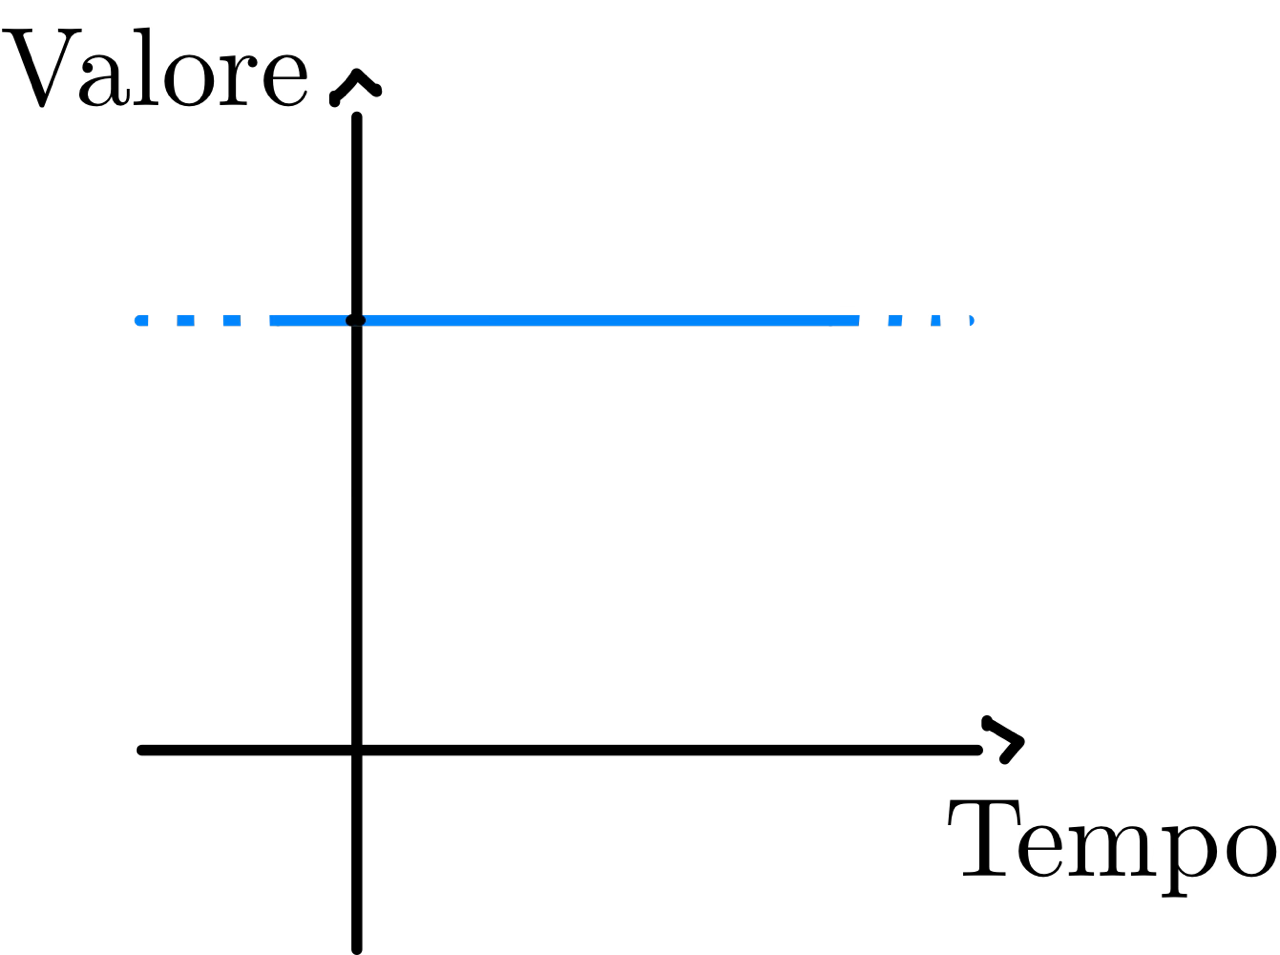
\includegraphics[width=0.2\textwidth]{src/book value.png}
                    \end{figure}
            \item \textit{Ammortamento}: progressivo storno del costo storico di un attività. L'importo non cancellato mostra la residura utilità dell'attività.
                    \begin{figure}[H]
                        \centering
                        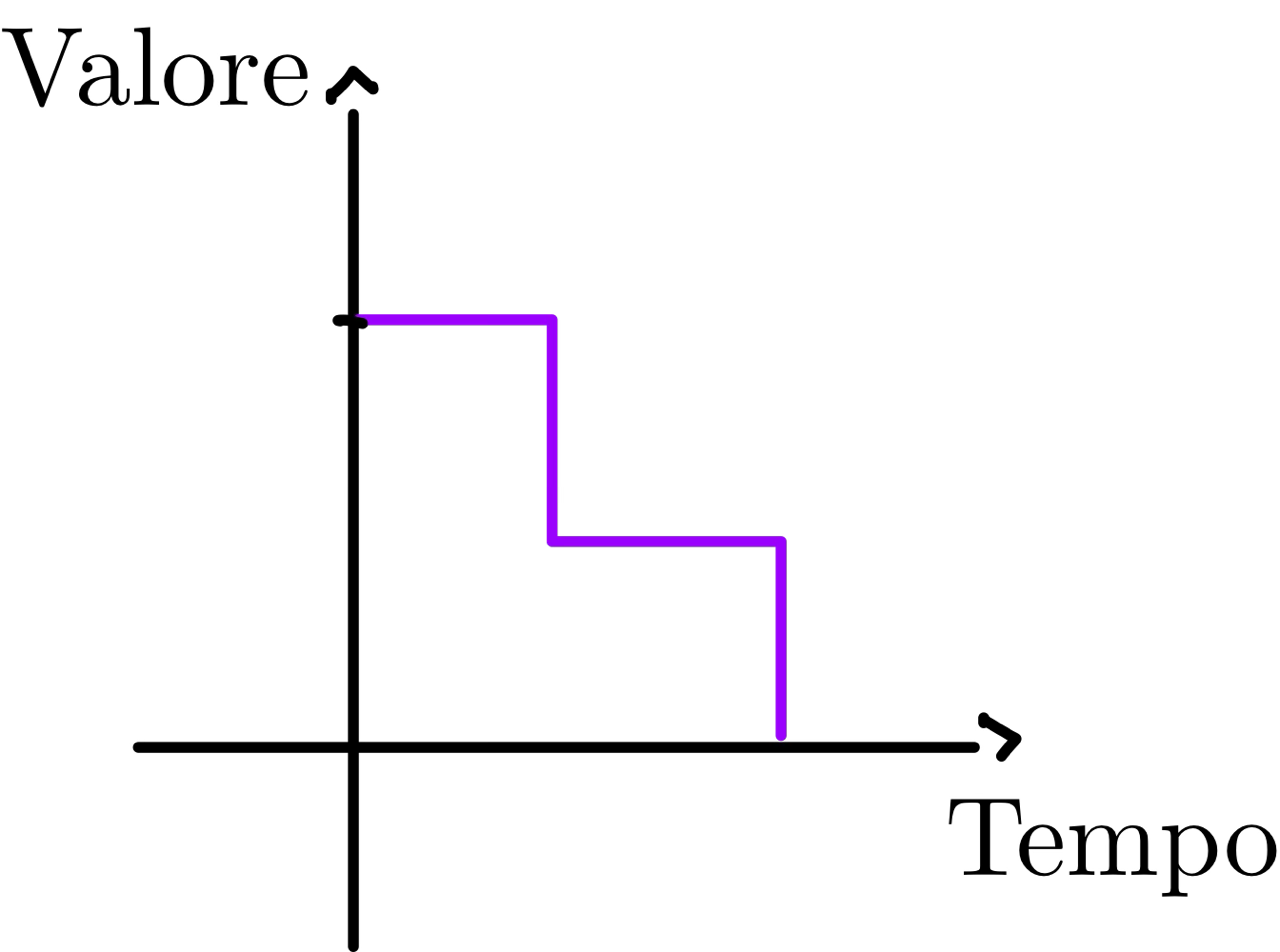
\includegraphics[width=0.2\textwidth]{src/ammortamento.png}
                    \end{figure}
            \end{itemize}
        \item \textbf{Attività monetarie}: vi è informazione oggettiva sul valore di mercato.
        \begin{itemize}
            \item \textit{Fair value}: l'attività viene contabilizzata al proprio valore di mercato.
        \end{itemize}
        \begin{figure}[h]
            \centering
            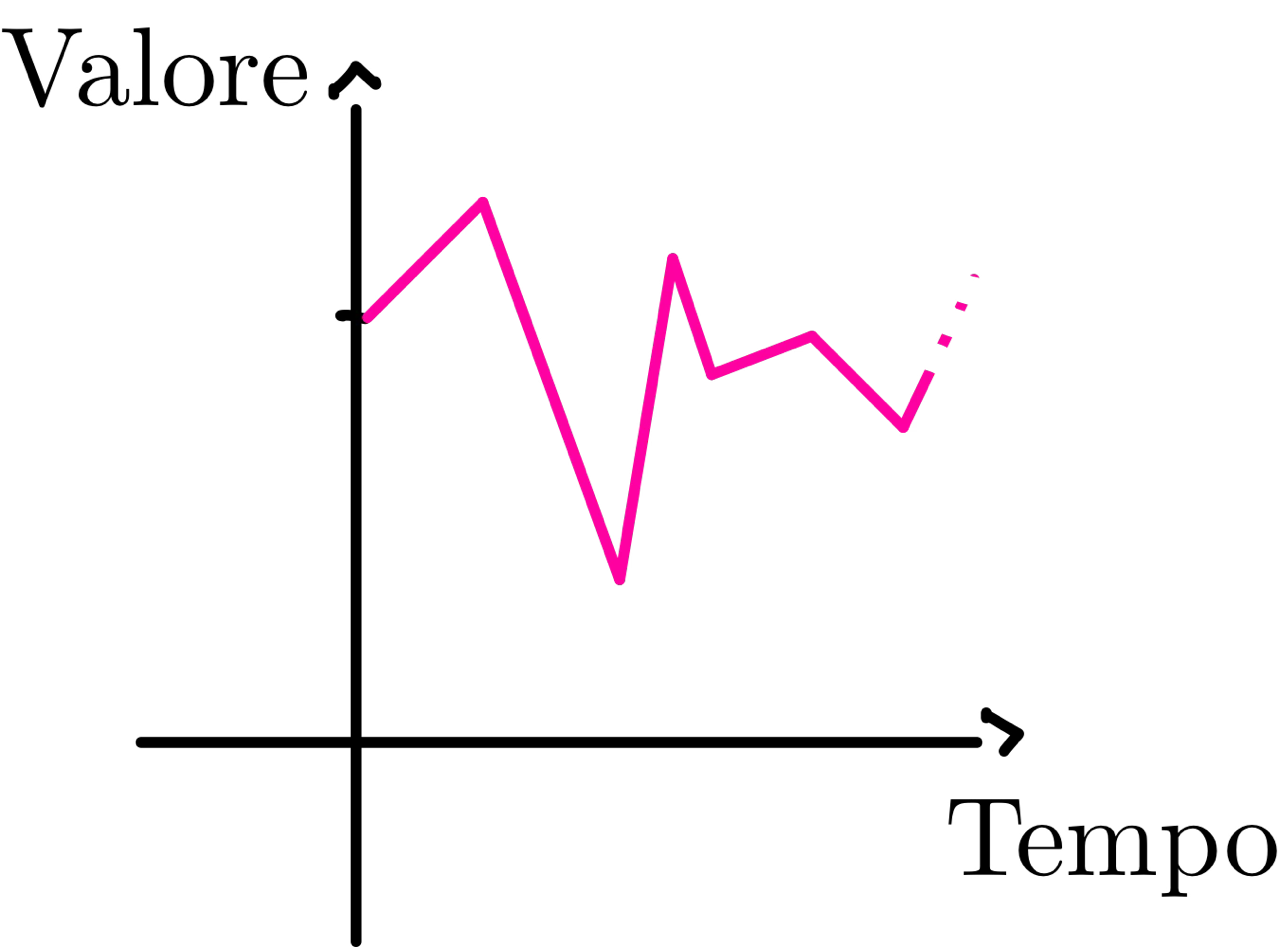
\includegraphics[width=0.2\textwidth]{src/fair value.png}
        \end{figure}
    \end{itemize}
    \item \textbf{Duplice aspetto}: ogni \textbf{transazione} produce un doppio effetto contabile necessario a mantenere l'equilibrio fondamentale tra attività (risorse) e fonti di finanziamento (passività più capitale netto). Questo principio sancisce l'uguaglianza secondo l'\textbf{equazione fondamentale della contabilità}: 
    $$ \text{attività} = \text{passività} + \text{capitale netto}$$
     Esso implica che ogni transazione deve essere registrata in modo da preservare tale equilibrio.
    \item \textbf{Periodicità della misurazione}: la contabilità misura periodicamente e on modo sistematico i risultati economici delle attività economiche, tale periodo è chiamato \textbf{esercizio}.
    \item \textbf{Prudenza}: 
    \begin{itemize}
        \item I \textbf{ricavi} devono essere registrati solo quando sono ragionevolmente \textbf{certi}.
        \item I \textbf{costi} devono essere registrate non appena sono ragionevolmente \textbf{probabili}.
    \end{itemize}
    \item \textbf{Realizzazione dei ricavi}: devono essere riconosciuti come ricavo l'ammontare che con ragionevole certezza il cliente pagherà.
    \item \textbf{Competenza}: i ricavi e i costi \textbf{correlati} devono essere registrati nello stesso esercizio.
    \item \textbf{Continuità dei criteri di valutazione}: i principi di contabilità devono rimanere costanti nel tempo.
    \item \textbf{Significatività e rilevanza}: Non si devono registrare eventi per i quali l'onere della contabilizzazione non sarebbe giustificato.
\end{enumerate}
\subsection{Rendiconti economico finanziari}
\subsubsection{Stato patrimoniale}
\setlength{\extrarowheight}{5pt} 
\begin{table}[H]
    \adjustbox{max width=\textwidth,center}{ 
        \begin{tabular}{|l|c|}
            \hline 
            \rowcolor{myblue} \color{white}\textbf{Stato Patrimoniale} & \color{white}\textbf{Risultati intermedi} \\
            \hline
                                                                          &                     \\
            Immobilizzazioni Materiali                                  &                     \\
            \hline
                                                                          &                     \\
            Immobilizzazioni Immateriali                                    &                     \\
            \hline
                                                                          &                     \\
            Immobilizzazioni Finanziarie                                  &                     \\
            \hline
            \textbf{Totale Immobilizzazioni}                              &                     \\
            \hline
                                                                          &                     \\
            Liquidità Immediate(e.g. cassa)                                           &                     \\
            \hline
                                                                          &                     \\
            Liquidità Differite(e.g. crediti a breve termine)                                           &                     \\
            \hline
                                                                          &                     \\                                                                         
            Rimanenze                                                     &                     \\
            
            \hline
            \textbf{Capitale Circolante}                                  &                     \\
            \hline
            \hline
            \textbf{Totale Attività}                                      &                     \\
            \hline
        \end{tabular}
        \begin{tabular}{|l|c|}
            \hline
            \rowcolor{myblue} \color{white} \textbf{Stato Patrimoniale}  &\color{white}  Risultati intermedi \\
            \hline
                                                                                      &                     \\
                                                                                      &                     \\
                                                                                      &                     \\
            Passività Consolidate, Medio/Lungo termine(e.g. mutui, fondo TFR)                                &                     \\
            \hline
                                                                                      &                     \\
                                                                                      &                     \\
                                                                                      &                     \\
            Passività Correnti, Breve termine (e.g. debiti vs fornitori)                                        &                     \\
            \hline
            \textbf{Passività}                                                        &                     \\
            \hline
            \hline
                                                                                      &                     \\
                                                                                      &                     \\
                                                                                      &                     \\
            (e.g. capitale sociale, utile)                                            &                     \\
            \hline
            \textbf{Capitale Netto = \textcolor{red}{ Valore Contabile}}               &                     \\
            \hline
            \hline
            \textbf{Totale Passività e Capitale Netto}                                &                     \\
            \hline
        \end{tabular}
    }
\end{table}
\subsubsection{Conto economico}
\begin{table}[H]
    \adjustbox{max width=\textwidth,center}{
            \begin{tabular}{|c|l|V{0.22\textwidth}|c|}
            \rowcolor{myblue}
            \hline
            \multicolumn{2}{|c|}{\color{white} \textbf{Conto Economico a costo del venduto}}&  \textbf{Note} &  \textbf{Sigla} \\
            \hline
            \textbf{A} & \textbf{Ricavi netti da vendite/servizi} & \tiny Valore dei beni/servizi consegnati nel periodo (netto di resi/sconti/imposte indirette). Base per analisi verticale.  & \\
            \textbf{B} & \textbf{Costo del venduto} & \tiny Costi \emph{diretti} riconducibili ad A (materie, MOD, lavorazioni esterne, quota logistica “inclusa”). \textbf{Escluso:} GA/Commerciali/R\&S. & \\
            \textbf{C = A - B} & \textbf{Margine lordo (Gross Profit)} & \tiny \textbf{RISULTATO INTERMEDIO}. Per pricing/mix/efficienza: se cala, verifica prezzo medio, sconti, scarti, produttività. & \textbf{GP} \\
            \hline

            & & \tiny Costi operativi \emph{ricorrenti} \textbf{esclusi D\&A}: Commerciali, Generali e Amm., logistica interna, R\&S, IT operativo. \textbf{Escluso:} finanza; accessoria; una tantum. & \\
            \textbf{D} & \textbf{Altri costi caratteristici (cash)} & & \\
            

            & & \tiny \textbf{RISULTATO INTERMEDIO} (performance “cash” dell’operatività). Utile per confronti con politiche d’ammortamento diverse. & \\
            \textbf{E = C - D} & \textbf{Margine Operativo Lordo (MOL)} & & \textbf{EBITDA (MOL)} \\
            \hline

            & & \tiny Quote non monetarie: ammortamenti materiali/immateriali; accantonamenti a fondi rischi. Non confondere con costi cash. & \\
            \textbf{F} & \textbf{Ammortamenti e accantonamenti (D\&A)} & & \\
            

            & & \tiny \textbf{RISULTATO INTERMEDIO} del core business \emph{al netto} di D\&A, prima della gestione accessoria. & \\
            \textbf{G = E - F} & \textbf{Risultato operativo caratteristico} & & \textbf{EBIT(RO)} \\
            \hline

            & & \tiny \textbf{Somma algebrica}: \textbf{+ proventi} (es. affitti attivi non core, servizi accessori, plus ordinarie), \textbf{$-$ oneri} (affitti passivi non core, penali/minus ordinarie). \textbf{Escluso:} finanza. & \\
            \textbf{H} & \textbf{Altri proventi/oneri operativi} & & \\
            

            & & \tiny \textbf{RISULTATO INTERMEDIO}. Core \emph{+} accessoria operativa (algebrico). Annota: “core X; accessoria Y” per leggibilità. & \\
            \textbf{I = G + H} & \textbf{Risultato operativo complessivo} & & \\
            \hline

            & & \tiny \textbf{Somma algebrica}: \textbf{+ proventi} (interessi attivi, rendite su tesoreria), \textbf{$-$ oneri} (interessi su debiti, commissioni/spese di funding). Tieni a lato il tasso effettivo: oneri fin. / debito medio. & \\
            \textbf{J} & \textbf{Proventi/oneri finanziari} & & \\
            

            & & \tiny \textbf{RISULTATO INTERMEDIO}. Operatività complessiva \emph{dopo} la finanza, \emph{prima} di non ricorrenti e imposte. Ottimo per confronti “puliti”. & \\
            \textbf{K = I + J} & \textbf{Risultato ordinario di competenza} & & \\
            \hline

            & & \tiny \textbf{Somma algebrica (facoltativa gestionale)}: \textbf{+ positivi} (es. indennizzi straordinari), \textbf{$-$ negativi} (es. incendio/furto, ristrutturazioni). Usa con giudizio e spiega sempre la causa. & \\
            \textbf{L} & \textbf{Componenti non ricorrenti (se evidenziati)} & & \\
            

            & & \tiny \textbf{RISULTATO INTERMEDIO}. Evidenzia qui l’effetto netto dei non ricorrenti. & \\
            \textbf{M = K + L} & \textbf{Risultato ante imposte} & & \textbf{EBT} \\
            \hline

            & & \tiny Imposte correnti + (eventuali) differite/anticipate. Specifica aliquote effettive e principali riconciliazioni. & \\
            \textbf{N} & \textbf{Imposte sul reddito d’esercizio} & & \\
            

            & & \tiny \textbf{RISULTATO INTERMEDIO FINALE}. Utile/Perdita di periodo. Aggiungi, se serve, EPS/utile per quota e destinazione risultato. & \\
            \textbf{O = M - N} & \textbf{Risultato netto} & & \textbf{NI} \\
            \hline
        \end{tabular}
    }
\end{table}

\subsubsection{Indici di bilancio}
\setlength{\extrarowheight}{15pt}
\begin{table}[H]
\centering
\small
\adjustbox{max width=\textwidth,center}{
\begin{tabular}{|Y{0.14\textwidth}|V{0.14\textwidth}|V{0.14\textwidth}|Y{0.30\textwidth}|V{0.18\textwidth}|}
\rowcolor{myblue}
\multicolumn{5}{|c|}{\color{white} \textbf{Analisi Reddituale per Indici}}\\
\hline
\textbf{Indicatore} & \textbf{Italiano} & \textbf{Inglese} & \textbf{Formula Standard} & \textbf{Note} \\
\hline
ROA(\%) & Redditività degli attivi & \textit{Return on Assets} & $\dfrac{\text{EBIT}}{\text{Totale Attività}}$ & \tiny \roaDesc \\
ROS(\%) & Redditività delle vendite & \textit{Return on Sales} & $\dfrac{\text{EBIT}}{\text{Ricavi}}$ & \tiny \rosDesc \\
ROE(\%) & Redditività del patrimonio & \textit{Return on Equity} & $\dfrac{\text{NI}}{\text{Capitale netto}}$ & \tiny \roeDesc \\
ROI(\%) & Redditività del capitale investito & \textit{Return on Investment} & $\dfrac{\text{EBIT}}{\text{Debiti finanziari}+\text{Capitale netto}}$ & \tiny \roiDesc \\
EPS & Utile per Azione & \textit{Earnings Per Share} & $\dfrac{\text{NI}}{\text{N.\ di azioni in circolazione}}$ & \tiny \epsDesc \\
\hline
\end{tabular}}
\end{table}

\begin{table}[H]
\centering
\small
\adjustbox{max width=\textwidth,center}{
\begin{tabular}{|V{0.14\textwidth}|V{0.14\textwidth}|Y{0.30\textwidth}|V{0.18\textwidth}|}
\hline
\rowcolor{myblue} \multicolumn{4}{|c|}{\color{white} \textbf{Analisi Finanziaria per Indici}}\\
\hline
\textbf{Indicatore} & \textbf{Inglese} & \textbf{Formula Standard} & \textbf{Note} \\
\hline
Indice di liquidità & \textit{Current ratio} & $\dfrac{\text{Attività correnti}}{\text{Passività correnti}}$ & \tiny \ilDesc \\
Indice di liquidità listretta & \textit{Acid test} & $\dfrac{\text{Attività correnti}-\text{Rimanenze}}{\text{Passività correnti}}$ & \tiny \ilrDesc \\
Tasso di indebitamento & \textit{Debt ratio} & $\dfrac{\text{Passività}}{\text{Attività}}$ & \tiny \tdDesc \\
Indice di indebitamento & \textit{Debt/Equity ratio} & $\dfrac{\text{Debiti finanziari}}{\text{Capitale netto}}$ & \tiny \iiDesc \\
Copertura interessi & \textit{Interest coverage} & $\dfrac{\text{EBIT}}{\text{Interessi passivi}}$ & \tiny \iciDesc \\
Grado di indebitamento & \textit{Indebtedness ratio} & $\dfrac{\text{Passività}}{\text{Capitale netto}}$ & \tiny \giDesc \\
Leva Finanziaria & \textit{Equity multiplier} & $\dfrac{\text{Attività}}{\text{Capitale netto}}$ & \tiny \lfDesc \\
\hline
\end{tabular}}
\end{table}

\begin{table}[H]
\centering
\small
\adjustbox{max width=\textwidth,center}{
\begin{tabular}{|V{0.14\textwidth}|V{0.14\textwidth}|Y{0.30\textwidth}|V{0.18\textwidth}|}
\hline
\rowcolor{myblue} \multicolumn{4}{|c|}{\color{white} \textbf{Analisi Strutturale e Rotazioni}}\\
\hline
\textbf{Indicatore} & \textbf{Inglese} & \textbf{Formula Standard} & \textbf{Note} \\
\hline
Rotazione delle rimanenze & \textit{Inventory turnover} & $\dfrac{\text{Costo del venduto}}{\text{Rimanenze}}$ & \tiny \rrDesc \\
Livello delle rimanenze (gg) & \textit{Days Inventory Outstanding (DIO)} & $\dfrac{\text{Rimanenze}}{\displaystyle \frac{\text{Costo del venduto}}{365}}$ & \tiny \lrDesc \\
Incasso cedio crediti commerciali (gg) & \textit{Days Sales Outstanding (DSO)} & $\dfrac{\text{Crediti commerciali}}{\displaystyle \frac{\text{Ricavi}}{365}}$ & \tiny \imccDesc \\
Giacenza media debiti commerciali (gg) & \textit{Days Payables Outstanding (DPO)} & $\dfrac{\text{Debiti verso fornitori}}{\displaystyle \frac{\text{Acquisti}}{365}}$ & \tiny \gmdcDesc \\
Capitale circolante netto (CCN) & \textit{Net Working Capital (NWC)} & $\text{Attività correnti}-\text{Passività correnti}$ & \tiny \ccnDesc \\
\hline
\end{tabular}}
\end{table}
\newpage
\section{Sistemi di controllo}
\subsection{Contabilità direzionale}
\begin{itemize}
    \item \textbf{Contabilità generale} : Processo di \textbf{rilevazione}, \textbf{misurazione}, \textbf{analisi}, \textbf{interpretazione} e \textbf{comunicazione} di informazioni che consentano agli utilizzatori (\textit{stakeholders}) di sviluppare \textbf{giudizi} e \textbf{decisioni} consapevoli riguardanti i loro rapporti con l’impresa.
    \item \textbf{Contabilità direzionale} : Processo che \textbf{produce informazioni},soprattutto quantitative, monetarie e non, utilizzate dal \textbf{management}, per favorire il raggiungimento degli obiettivi dell'organizzazione.\begin{itemize}
              \item \textbf{Programmazione} : definizione degli obiettivi e delle strategie per raggiungerli, attraverso la \textbf{pianificazione} delle attività, chiamato anche \textbf{budgeting}.
              \item \textbf{Implementazione} : attuazione delle decisioni prese.
              \item \textbf{Controllo} : verifica che le attività siano svolte in modo conforme alle decisioni prese.
          \end{itemize}
\end{itemize}
\subsection{Contabilità direzionale vs contabilità generale}
\begin{table}[H]
    \setlength{\extrarowheight}{12pt}
    \adjustbox{max width=\textwidth,center}{
        \centering
        \begin{tabular}{|l|l|l|}
            \hline
            \rowcolor{myblue}
            \textbf{Caratteristiche}       & \textbf{Contabilità direzionale}                       & \textbf{Contabilità generale}                             \\
            \hline
            \textbf{Necessità            } & Facoltativa                                            & Obbligatoria                                              \\
            \hline
            \textbf{Finalità             } & Strumento per assisitere il management nelle decisioni & Strumento per assisitere gli stakeholders nelle decisioni \\
            \hline
            \textbf{Utenti               } & Management (noti)                                      & Stakeholders (ignoti)                                     \\
            \hline
            \textbf{Struttura sottostante} & Cambia in base alle esigenze                           & Struttura fissa ($A = P + CN$)                            \\
            \hline
            \textbf{Fonte dei principi   } & Qualsiasi sia utile                                    & Codice civile e Principi contabili                        \\
            \hline
            \textbf{Prospettiva          } & Storica e prospettica                                  & Storica                                                   \\
            \hline
            \textbf{Tipo di informazioni } & Quantitative e qualitative, prevalentemente monetarie  & Quantitative, monetarie                                   \\
            \hline
            \textbf{Precisione           } & Bassa                                                  & Alta                                                      \\
            \hline
            \textbf{Periodicità          } & Qualsiasi sia utile                                    & Annuale                                                   \\
            \hline
            \textbf{Tempestività         } & Qualsiasi sia utile                                    & Entro 120 giorni dalla chiusura dell'esercizio            \\
            \hline
            \textbf{Oggetto              } & Impresa ma anche singoli prodotti, clienti, ecc.       & Impresa                                                   \\
            \hline
            \textbf{Responsabilità       } & Virtualmente nessuna                                   & Sempre presente                                           \\
            \hline
        \end{tabular}
    }
    \caption{Contabilità direzionale vs contabilità generale}
\end{table}
\subsection{I 3 scopi e i 3 modi di considerare i costi}
\begin{itemize}
    \item \textbf{Misurazione} $\Rightarrow$ \textbf{Costo pieno} : \textbf{costo} di un prodotto o servizio, \textbf{somma} di tutti i costi sostenuti per produrlo o fornirlo.
    \item \textbf{Controllo} $\Rightarrow$ \textbf{Costo per centro di responsabilità} : \textbf{costo} di un centro di responsabilità, \textbf{somma} di tutti i costi sostenuti per gestirlo.
    \item \textbf{Decisione} $\Rightarrow$ \textbf{Costo differenziale} : \textbf{costo} di una decisione, \textbf{differenza} tra i costi alternativi.
\end{itemize}

\subsection{Classificazione dei costi in funzione del loro comportamento}
\begin{itemize}
    \item \textbf{Costi variabili totali} (CVT): costi che variano in proporzione al volume di produzione.
        \begin{figure}[H]
            \centering
            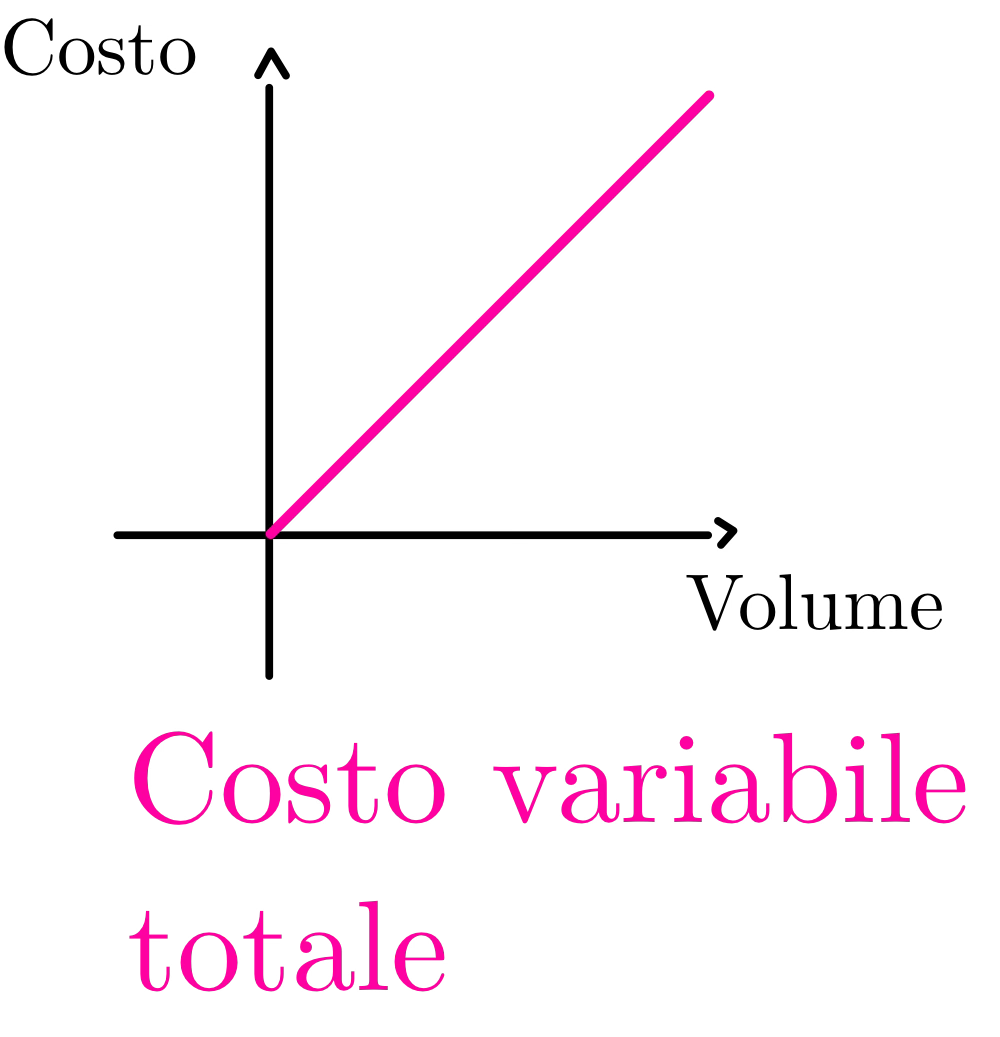
\includegraphics[width=0.2\textwidth]{src/costo variabile.png}
        \end{figure}
    \item \textbf{Costi fissi totali} (CFT): costi che non variano in proporzione al volume di produzione, si dividono in:
          \begin{itemize}
              \item \textbf{Costi impegnati (costi da capacità)}: costi  dotano l’azienda di una certa \textbf{“capacità produttiva”}, la quale perdura fino alla dismissione della relativa risorsa impegnata, sono irreversibili.
              \item \textbf{Costi discrezionali}: costi che l’azienda può decidere di sostenere o meno durante la fase di \textbf{"budgeting"} sono reversibili.
          \end{itemize}
        \begin{figure}[H]
            \centering
            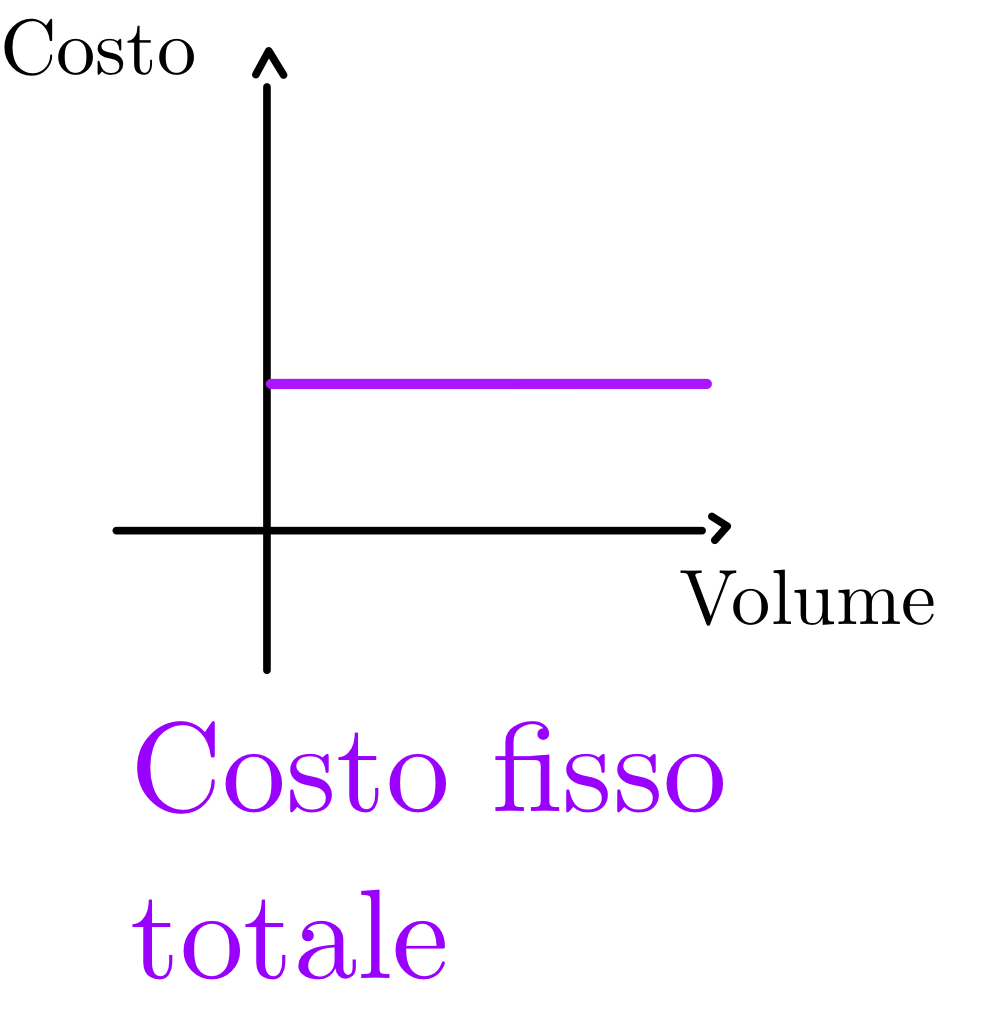
\includegraphics[width=0.2\textwidth]{src/costo fisso.png}
        \end{figure}
    \item \textbf{Costi semivariabili} : costi che sono un mix di costi fissi e costi variabili.
    \begin{figure}[H]
            \centering
            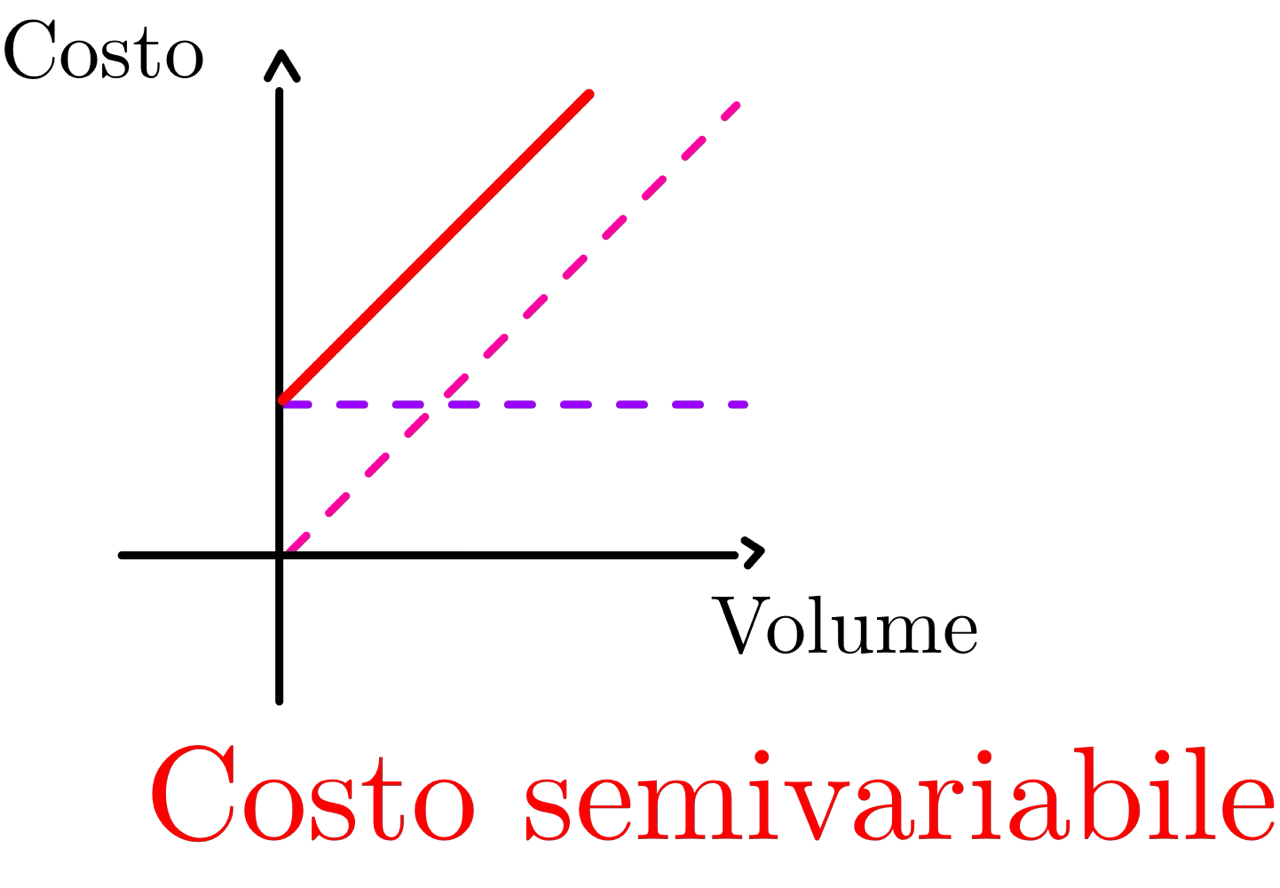
\includegraphics[width=0.2\textwidth]{src/costo semivariabile.png}
    \end{figure}
    \item \textbf{Costi viscosi} : costi che variano in modo discontinuo, crescono rapidamente in risposta a un aumento del volume di produzione, ma diminuiscono lentamente in risposta a una diminuzione del volume di produzione.
    \begin{figure}[H]
            \centering
            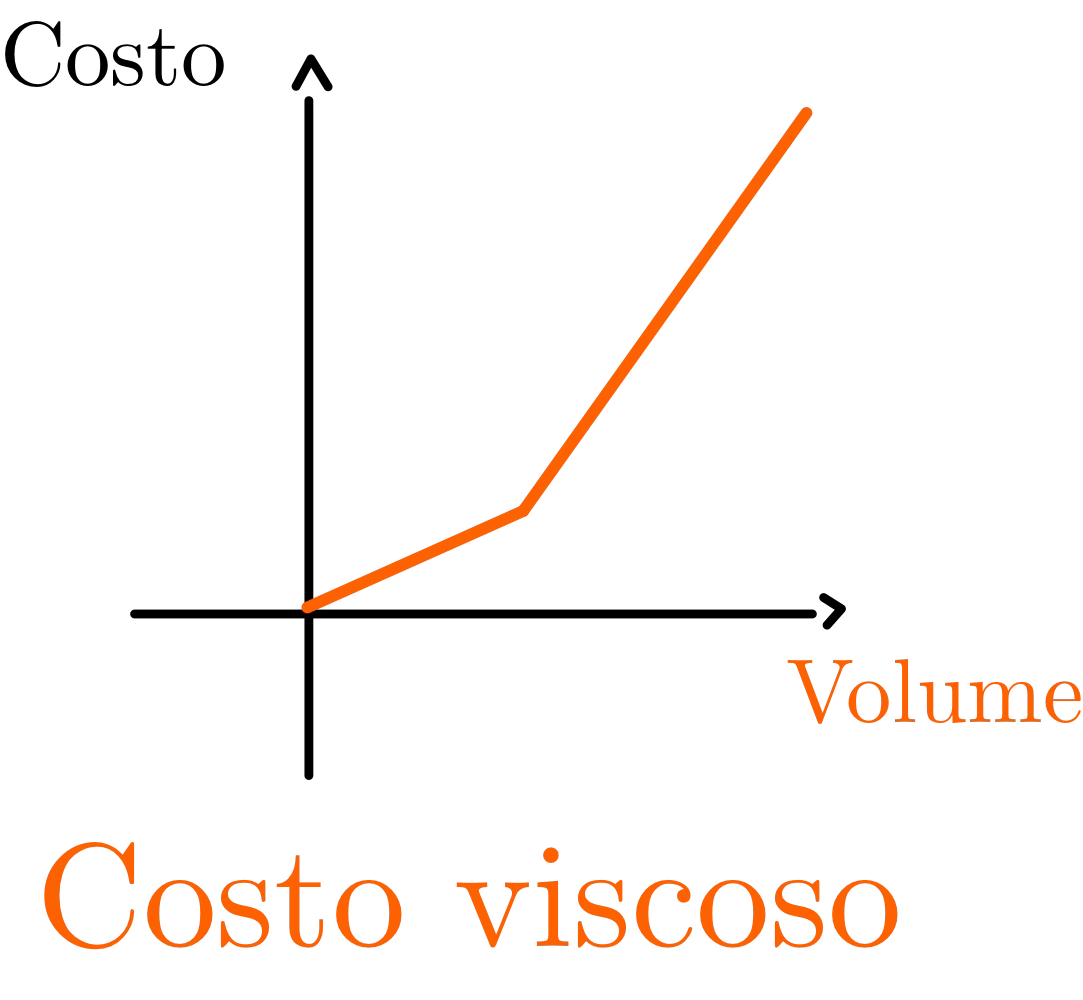
\includegraphics[width=0.2\textwidth]{src/costo viscoso.png}
    \end{figure}
    \item \textbf{Costi a gradino} : costi riferiti a risorse che possono essere acquistate o vendute solo in quantità discrete.
    \begin{figure}[H]
            \centering
            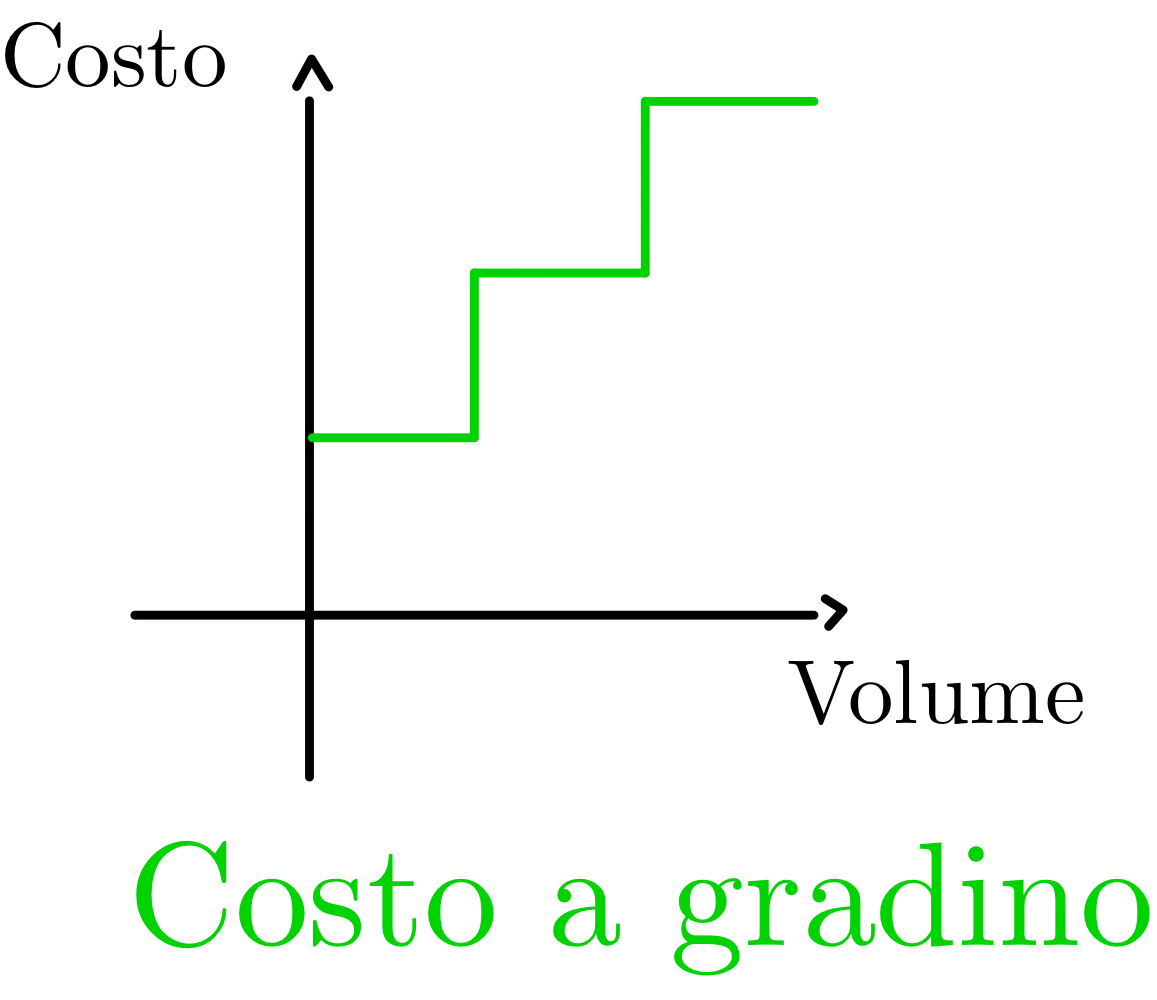
\includegraphics[width=0.2\textwidth]{src/costo a gradino.png}
    \end{figure}
\end{itemize}
\begin{table}[H]
    \setlength{\extrarowheight}{10pt}
    \adjustbox{max width=\textwidth,center}{
        \centering
        \begin{tabular}{|l|l|l|l|}
            \hline
            \rowcolor{myblue}
            \textbf{Costo}           & \textbf{Equazione}                & \textbf{Spiegazione}                                    & \textbf{Osservazioni}                                                                 \\
            \hline
            Volume                   & $X$                               & Volume di produzione                                    & $\textcolor{myblue}{x}$                                                               \\
            \hline
            Costo variabile unitario & $cvu$                             & Costo per unità prodotta                                & $\textcolor{myblue}{m}$                                                               \\
            \hline
            Costo variabile totale   & $CVT = cvu \cdot X$               & Costi \textbf{complessivamente} proporzionali al volume & $CVT(\textcolor{myblue}{x}) = cvu \cdot \textcolor{myblue}{x}$                        \\
            \hline
            Costo fisso totale       & $CFT$                             & Costi \textbf{non} proporzionali al volume              & $CFT = \textcolor{myblue}{q}$                                                         \\
            \hline
            Costo totale             & $CT = CFT + cvu \cdot X$          & Somma dei costi \textbf{fissi} e \textbf{variabili}     & $CT(\textcolor{myblue}{x}) = CFT + cvu \cdot \textcolor{myblue}{x}$                   \\
            \hline
            Costo medio unitario     & $CMU = \displaystyle\frac{CT}{X}$ & Costo medio per unità prodotta                          & $\displaystyle CMU(\textcolor{myblue}{x}) = \frac{CFT} {\textcolor{myblue}{x}} + cvu$ \\
            \hline
        \end{tabular}
    }
    \caption{Costi}
\end{table}
\begin{figure}[H]
    \centering
    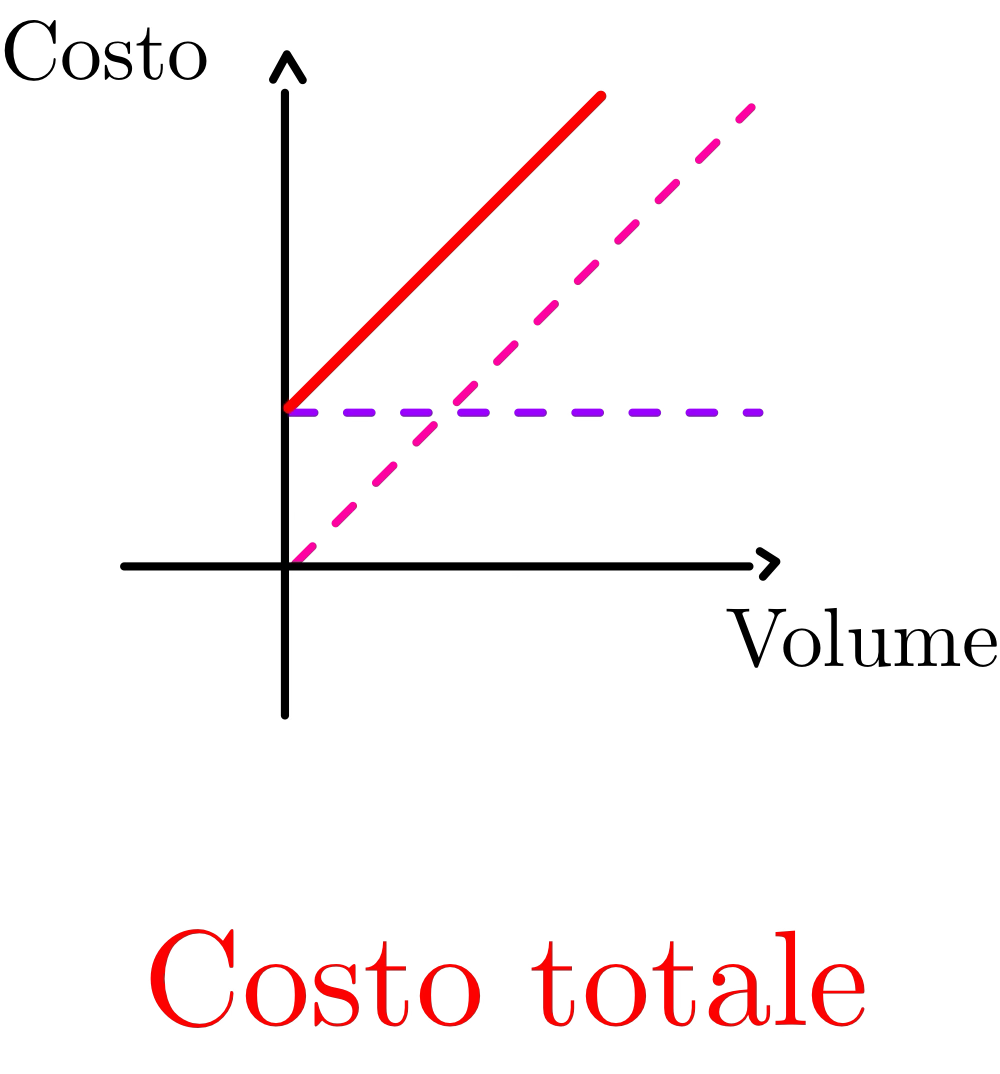
\includegraphics[width=0.4\textwidth]{src/costo totale.png}
\end{figure}
\subsection{Costo medio unitario}
Il costo medio unitario è il costo medio per unità prodotta,
\begin{align*}
     & CMU                         = \frac{CT}{X} = \frac{CFT}{X} + cvu                                                                                                                                                                                    \\                                                                                                                          \\
     & CMU(\textcolor{myblue}{x})  =\frac{CT}{\textcolor{myblue}{x}} = \frac{CFT + CVT }{\textcolor{myblue}{x}}=\frac{CFT}{\textcolor{myblue}{x}} + \frac{cvu \cdot \textcolor{myblue}{x}}{\textcolor{myblue}{x}} =\frac{CFT}{\textcolor{myblue}{x}} + cvu \\
\end{align*}
\begin{figure}[H]
    \centering
    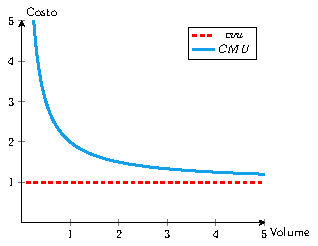
\includegraphics[width=0.4\textwidth]{tikz/costo medio unitario.pdf}
    \caption{Costo medio unitario}
\end{figure}
\subsection{Margine di contribuzione}
\subsubsection{Ricavo unitario o Prezzo di vendita}
\begin{align*}
     & p \quad \text{o} \quad r_u
\end{align*}
È il ricavo ottenuto dalla vendita di una singola unità di prodotto.
\subsubsection{Ricavo totale}
\begin{align*}
     & RT =  p \cdot X                                              \\
     & RT(\textcolor{myblue}{x}) =  p \cdot (\textcolor{myblue}{x})
\end{align*}
Indica il ricavo complessivo ottenuto dalla vendita di $X$ unità di prodotto.
\subsubsection{Margine di contribuzione unitario}
\begin{align*}
     & MdC_u = (p - cvu) \\
\end{align*}
È la differenza tra il prezzo di vendita unitario e il costo variabile unitario.
\subsubsection{Margine di contribuzione totale}
\begin{align*}
     & MdC_u =  RT - CVT =  (p - cvu) \cdot X                                                                                          \\
     & MdC(\textcolor{myblue}{x}) =  RT(\textcolor{myblue}{x}) - CVT(\textcolor{myblue}{x}) =  (p - cvu) \cdot (\textcolor{myblue}{x})
\end{align*}
Rappresenta il contributo totale alla copertura dei costi fissi e al profitto.
\subsubsection{Margine di contribuzione percentuale}
\begin{align*}
     & \text{MCP} = \left( \frac{MdC_u}{p} \right) \cdot 100                            \\
     & \text{MCP}(\textcolor{myblue}{x}) = \left( \frac{(p - cvu)}{p} \right) \cdot 100
\end{align*}
Indica quale percentuale del prezzo di vendita per unità rimane dopo aver coperto i costi variabili unitari. È utile per determinare quanto ogni unità venduta contribuisca, in termini percentuali, alla copertura dei costi fissi e alla generazione di profitto.
\subsubsection{Margine di sicurezza}
\begin{align*}
     & MS = X - X_P = X - \frac{CFT}{MdC_u} = \frac{MdC_u \cdot X - CFT}{MdC_u} = \frac{MdC - CFT}{MdC_u}                                                                             \\
     & MS(\textcolor{myblue}{x}) = \textcolor{myblue}{x} - \frac{CFT}{MdC_u} = \frac{MdC_u \cdot \textcolor{myblue}{x} - CFT}{MdC_u} = \frac{MdC(\textcolor{myblue}{x}) - CFT}{MdC_u}
\end{align*}
Rappresenta di quanto il volume attuale eccede il volume di pareggio.
\subsubsection{Utile o Profitto}
\begin{align*}
     & P = RT - CT = MdC - CFT = (p - cvu) \cdot X  - CFT                                                        \\
     & P(\textcolor{myblue}{x}) = MdC(\textcolor{myblue}{x}) - CFT = (p - cvu) \cdot (\textcolor{myblue}{x})-CFT
\end{align*}
È la differenza tra il ricavo totale e il costo totale.
\subsubsection{Volume di pareggio (Break-even volume)}
\begin{align*}
     & P(\textcolor{myblue}{x}) = 0                               \\
     & (p - cvu) \cdot (\textcolor{myblue}{x})-CFT = 0            \\
     & (p - cvu) \cdot (\textcolor{myblue}{x}) = CFT              \\
     & (\textcolor{myblue}{x}) = \displaystyle\frac{CFT}{(p-cvu)} \\
     & X_p = \displaystyle\frac{CFT}{MdC_u} = \frac{CFT}{(p-cvu)}
\end{align*}
Indica il volume di produzione necessario per coprire tutti i costi, generando un profitto nullo.
\subsubsection{Volume per ottenere un profitto obiettivo}
\begin{align*}
     & P(\textcolor{myblue}{x}) = P_O                                             \\
     & (p - cvu) \cdot (\textcolor{myblue}{x})-CFT = P_O                          \\
     & (p - cvu) \cdot (\textcolor{myblue}{x}) = CFT + P_O                        \\
     & (\textcolor{myblue}{x}) = \displaystyle\frac{CFT + P_O}{(p-cvu)}           \\
     & X_{P_O} = \displaystyle\frac{CFT + P_O}{MdC_u} = \frac{CFT + P_O}{(p-cvu)}
\end{align*}
È il volume di produzione necessario per raggiungere un profitto obiettivo $P_O$.
\subsubsection{Leva operativa}
L'effetto leva è misurato dal grado di leva operativa, che è il rapporto tra il margine di contribuzione e il profitto.
\begin{align*}
     & \text{Grado di leva operativa} = \frac{MdC}{P} = \frac{MdC_u \cdot X}{MdC_u \cdot X - CFT} = \frac{(p-cvu) X}{(p-cvu) X - CFT}                                                                                                                                                                                                                 \\
     & \text{Grado di leva operativa}(\textcolor{myblue}{x}) = \displaystyle\frac{MdC(\textcolor{myblue}{x})}{P(\textcolor{myblue}{x})} = \displaystyle\frac{MdC_u \cdot (\textcolor{myblue}{x})}{MdC_u \cdot (\textcolor{myblue}{x}) - CFT} = \displaystyle\frac{(p-cvu) \cdot (\textcolor{myblue}{x})}{(p-cvu) \cdot (\textcolor{myblue}{x}) - CFT} \\
\end{align*}
Indica di quanto varia il margine di contribuzione per unità di prodotto in risposta a una variazione del volume di produzione.
\subsection{Incidenza percentuale delle quantità di vendita di un prodotto sulle quantità complessive}
\begin{align*}
     & I_{\% a} = \frac{X_a}{X_T} \cdot 100                                                \\
     & I_{\% (\textcolor{myblue}{x})} = \frac{(\textcolor{myblue}{x})}{\sum X_i} \cdot 100
\end{align*}
\subsubsection{Margine di contribuzione equivalente}
\begin{align*}
     & MdC_e = \displaystyle MdC_a \cdot I_{\% a} + MdC_b \cdot I_{\% b} = (p_a - cvu_a) \cdot I_{\% a} + (p_b - cvu_b) \cdot I_{\% b} \\
\end{align*}
Se l'azienda ha più prodotti, il margine di contribuzione equivalente è la somma dei margini di contribuzione di tutti i prodotti, pesati per l'incidenza percentuale delle quantità di vendita di un prodotto sulle quantità complessive.
\subsubsection{Tempo di produzione totale di produzione o Tempo macchina}
Indica il tempo di utilizzo di una macchina.
\subsubsection{Tempo di produzione unitario}
\begin{align*}
     & T_u = \text{Tempo di produzione unitario} = \frac{\text{Tempo totale di produzione}}{\text{Numero di unità prodotte}} = \frac{\text{Tempo totale di produzione}}{(\textcolor{myblue}{x})} \\
     & T_u = \text{Tempo di produzione unitario} = \frac{1}{\text{Produttività oraria}} = \frac{1}{P_h}                                                                                          \\
\end{align*}
Indica il tempo necessario per produrre una singola unità di prodotto.
\subsubsection{Produttività oraria}
\begin{align*}
     & P_h = \text{Produttività oraria} = \frac{\text{Numero di unità prodotte}}{\text{Tempo totale di produzione}} = \frac{(\textcolor{myblue}{x})}{\text{Tempo totale di produzione}} \\
     & P_h = \text{Produttività oraria} = \frac{1}{\text{Tempo di produzione unitario}} = \frac{1}{T_u}                                                                                 \\
\end{align*}
Indica il numero di unità prodotte in un'ora.
\subsubsection{Margine di contribuzione orario}
\begin{align*}
     & MdC_h = \text{Margine di contribuzione orario} = \displaystyle\frac{MdC_{u}}{T_{u}} = MdC_u \cdot P_h \\
\end{align*}
Indica il margine di contribuzione per unità di tempo.
Lo uso quando negli esercizi mi viene dato un tempo macchina limite e devo capire quale mix di prodotti mi permette di massimizzare il margine di contribuzione.
\begin{table}[H]
    \setlength{\extrarowheight}{12pt}
    \adjustbox{max width=\textwidth,center}{
        \centering
        \begin{tabular}{|l|l|l|}
            \hline
            \rowcolor{myblue}
            \textbf{Voce}                                                       & \textbf{Spiegazione}                                                  & \textbf{Osservazioni}                                                                                                                                                                                                         \\
            \hline
            Ricavo unitario o Prezzo di vendita                                 & Ricavo per unità prodotta                                             & $\textcolor{myblue}{m}$                                                                                                                                                                                                       \\
            \hline
            Ricavo totale                                                       & Ricavi \textbf{complessivamente} proporzionali al volume              & $RT(\textcolor{myblue}{x}) = p \cdot \textcolor{myblue}{x}$                                                                                                                                                                   \\
            \hline
            Margine di contribuzione unitario                                   & Margine di contribuzione per unità prodotta                           & $MdC_u = (p - cvu)$                                                                                                                                                                                                           \\
            \hline
            Margine di contribuzione                                            & Ricavo totale - Costo variabile totale                                & $MdC(\textcolor{myblue}{x}) = RT(\textcolor{myblue}{x}) - CVT(\textcolor{myblue}{x}) = (p-cvu)(\textcolor{myblue}{x})$                                                                                                        \\
            \hline
            Margine di contribuzione percentuale                                & Percentuale del ricavo netto dai costi variabili per unità            & $ MdC_{\%}(\textcolor{myblue}{x}) = \left( \displaystyle\frac{(p - cvu)}{p} \right) \cdot 100$                                                                                                                                \\
            \hline
            Utile o Profitto                                                    & Ricavo totale - Costo totale                                          & $P(\textcolor{myblue}{x}) = MdC(\textcolor{myblue}{x}) - CFT = (p - cvu)(\textcolor{myblue}{x})-CFT$                                                                                                                          \\
            \hline
            Volume di pareggio                                                  & Volume di produzione per cui il profitto è nullo                      & $ (\textcolor{myblue}{x}) = \displaystyle\frac{CFT}{(p-cvu)}$                                                                                                                                                                 \\
            \hline
            Voleme per ottenere un profitto obiettivo $\textcolor{myblue}{P_O}$ & Volume di produzione per cui il profitto è $\textcolor{myblue}{P_O}$  & $ (\textcolor{myblue}{x}) = \displaystyle\frac{CFT + \textcolor{myblue}{P_O}}{(p-cvu)}$                                                                                                                                       \\
            \hline
            Grado di leva operativa                                             & Rapporto tra margine di contribuzione e profitto                      & $\text{Grado di leva}(\textcolor{myblue}{x}) = \displaystyle\frac{MdC(\textcolor{myblue}{x})}{P(\textcolor{myblue}{x})} = \displaystyle\frac{MdC_u \cdot (\textcolor{myblue}{x})}{MdC_u \cdot (\textcolor{myblue}{x}) - CFT}$ \\
            \hline
            Incidenza                                                           & Percentuale di un prodotto sul totale                                 & $I_{\% (\textcolor{myblue}{x})} = \displaystyle\frac{(\textcolor{myblue}{x})}{\sum X_i}$                                                                                                                                      \\
            \hline
            Margine di contribuzione equivalente                                & Somma dei margini di contribuzione pesati per l'incidenza percentuale & $MdC_e = \displaystyle MdC_a \cdot \frac{X_a}{X_{tot}} + MdC_b \cdot \frac{X_b}{X_{tot}}$                                                                                                                                     \\
            \hline
            Tempo di produzione unitario                                        & Tempo necessario per produrre una singola unità di prodotto           & $T_u = \displaystyle\frac{\text{Tempo totale di produzione}}{(\textcolor{myblue}{x})} = \displaystyle \frac{1}{P_h}$                                                                                                          \\
            \hline
            Produttività oraria                                                 & Numero di unità prodotte in un'ora                                    & $P_h = \displaystyle\frac{(\textcolor{myblue}{x})}{\text{Tempo totale di produzione}} = \displaystyle \frac{1}{T_u} $                                                                                                         \\
            \hline
            Margine di contribuzione orario                                     & Margine di contribuzione per unità di tempo                           & $MdC_h = \displaystyle\frac{MdC_{u}}{T_{u}} = MdC_u \cdot P_h$                                                                                                                                                                \\
            \hline
        \end{tabular}
    }
    \caption{Tabella di analisi del margine di contribuzione}
\end{table}

\subsection{Diagrammi di costo,ricavo e utile}
Il \textbf{break even point (BEP)} è il punto in cui i ricavi totali e i costi totali si intersecano, ovvero il punto in cui l'azienda non realizza né un profitto né una perdita.
\begin{figure}[H]
    \centering
    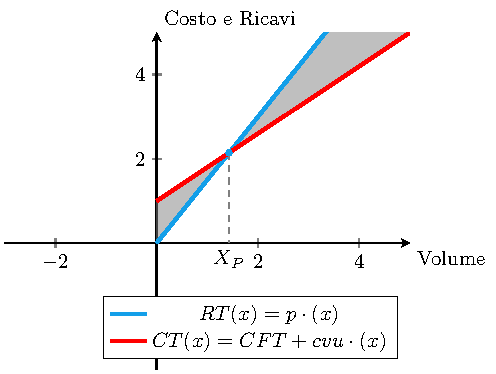
\includegraphics[width=0.5\textwidth]{tikz/costo ricavi.pdf}
    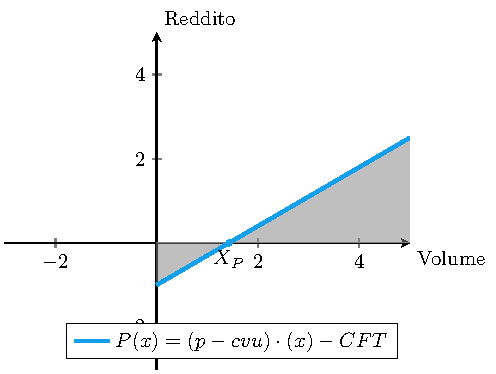
\includegraphics[width=0.5\textwidth]{tikz/utile.pdf}
    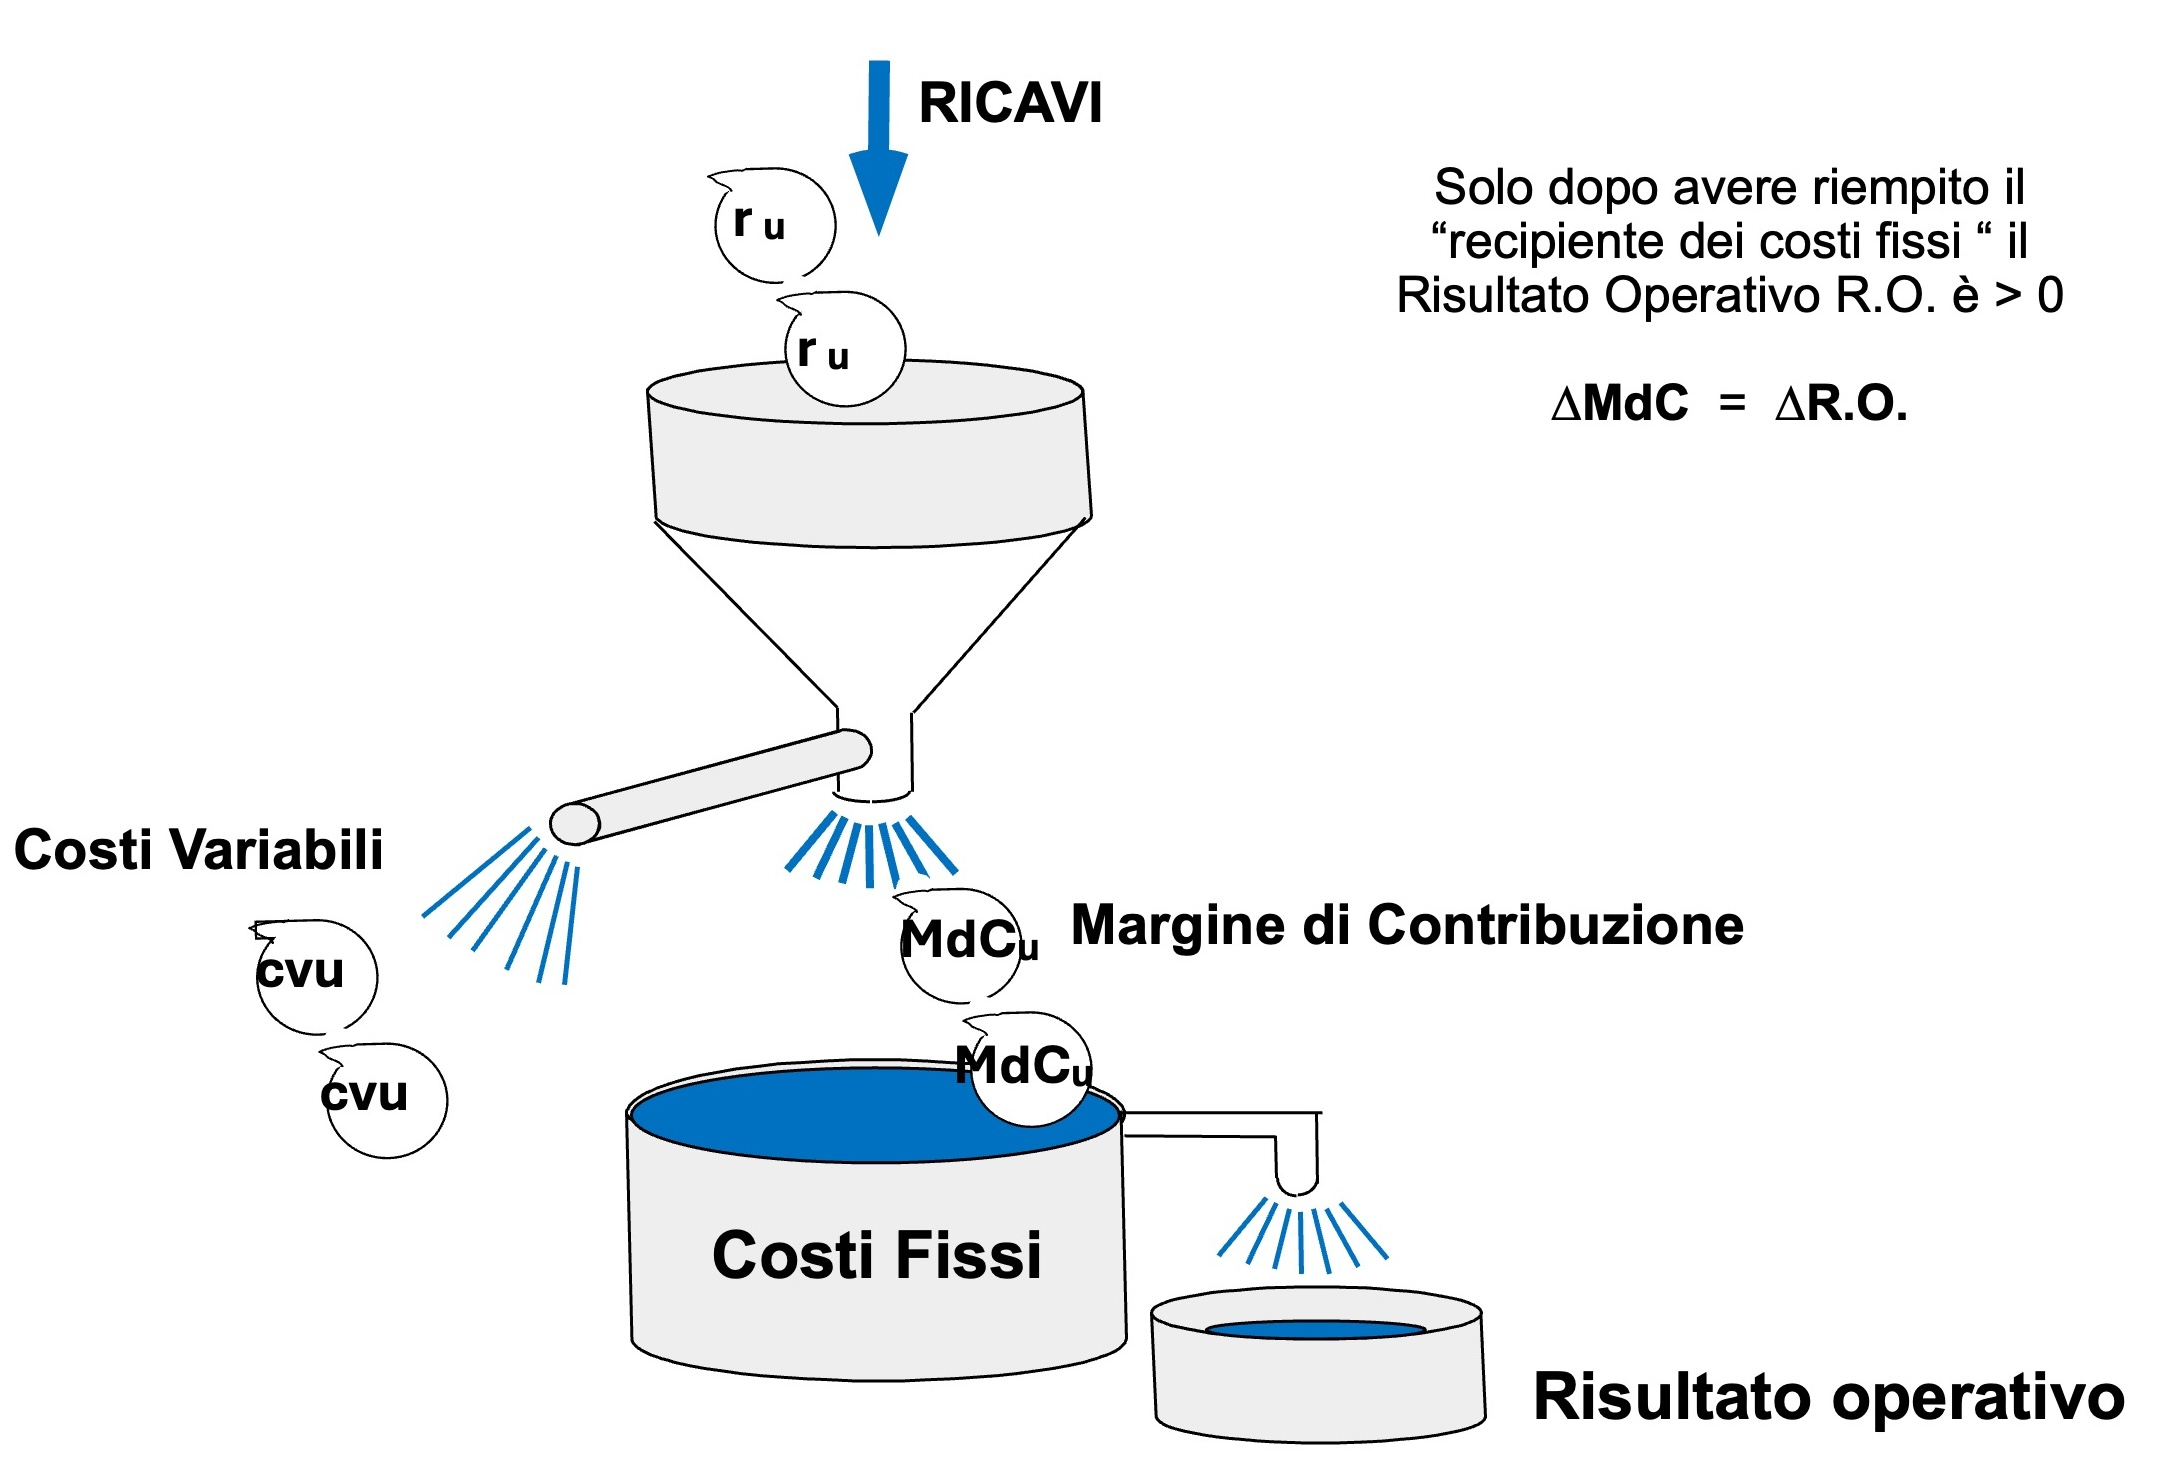
\includegraphics[width=0.7\textwidth]{src/margine di contribuzione.jpg}
    \caption{Margine di contribuzione e Reddito}
\end{figure}

\subsection{Conto economico a margine di contribuzione}
\'E un rendiconto preparato per valutare rapidamente l'effetto sul reddito di cambiamenti delle quantit\'a vendute o dei ricavi.
\begin{figure}[H]
    \centering
    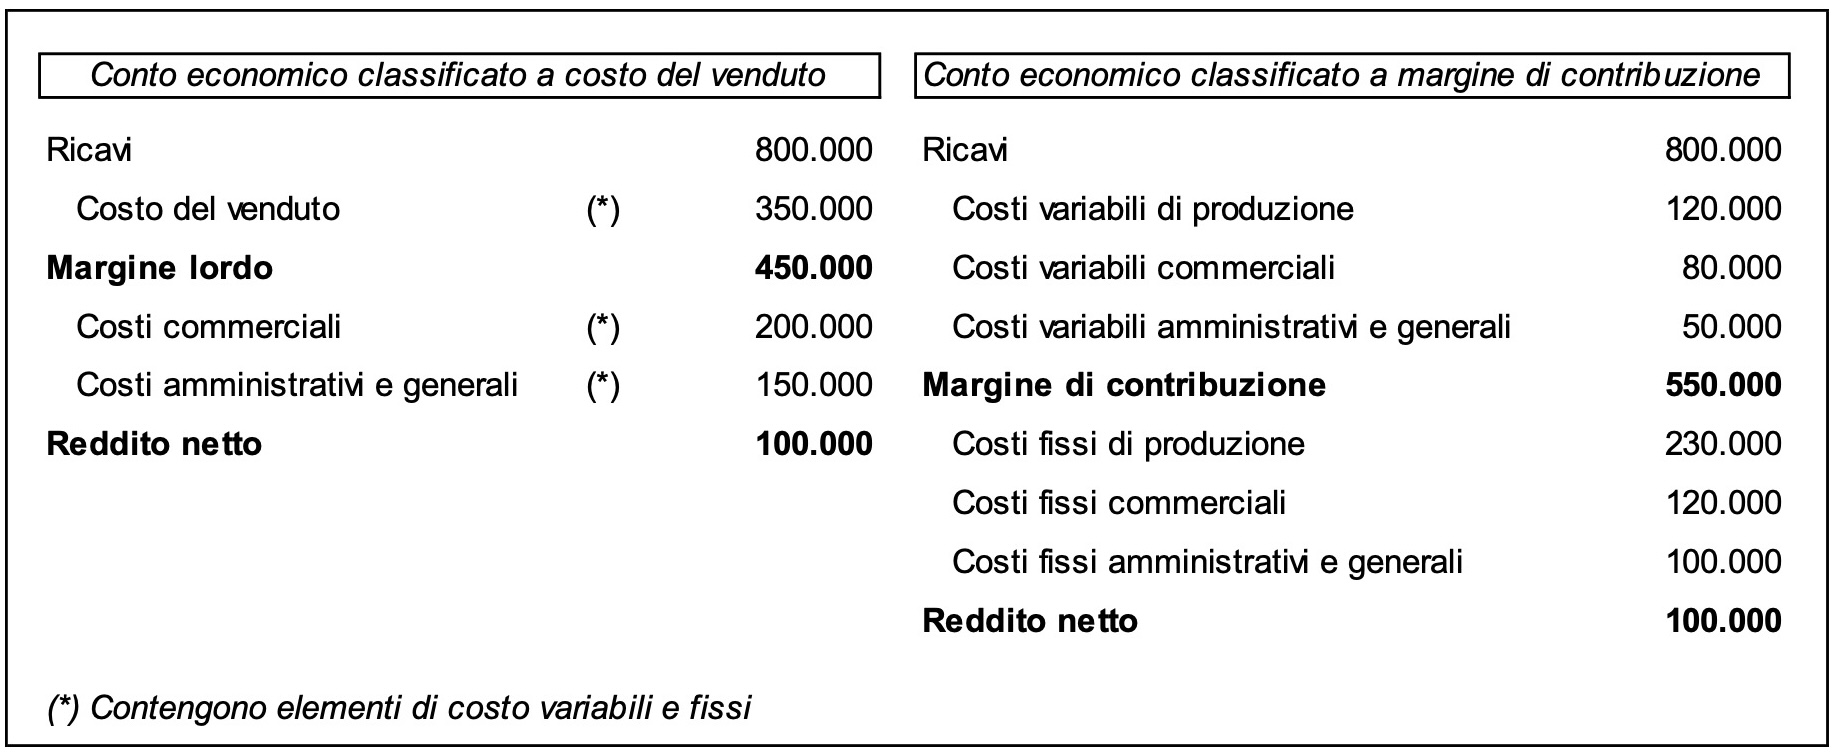
\includegraphics[width=0.8\textwidth]{src/conto economico a margine di contribuzione.jpg}
    \caption{Conto economico a margine di contribuzione}
\end{figure}
\begin{table}[H]
    \setlength{\extrarowheight}{12pt}
    \adjustbox{max width=\textwidth,center}{
        \centering
        \begin{tabular}{|l|l|l|}
            \hline
            \rowcolor{myblue}
            \textbf{Voce}                     & \textbf{Spiegazione}                   & \textbf{Voce}    \\
            \hline
            Ricavi                            & Ricavi totali                          & $RT$             \\
            Costi variabili                   & Costi variabili totali                 & $CVT$            \\
            \textbf{Margine di contribuzione} & Ricavi - Costi variabili               & $MdC = RT - CVT$ \\
            \hline
            Costi fissi totali                & Costi fissi totali                     & $CFT$            \\
            \textbf{Utile o Profitto}         & Margine di contribuzione - Costi fissi & $RT= MdC - CFT$  \\
            \hline
        \end{tabular}
    }
    \caption{Conto economico a margine di contribuzione}
\end{table}
\subsection{Costi pieni}
\begin{itemize}
    \item \textbf{Costo} : \textbf{valorizzazione monetaria} delle risorse consumate per conseguire uno \textbf{scopo},(\textbf{Oggetto del costo}).
    \item \textbf{Costo pieno} : somma di :
          \begin{itemize}
              \item \textbf{Costo diretto} : costo che può essere \textbf{direttamente} ricondotto all’oggetto del costo.
              \item \textbf{Costo indiretto} : costo che \textbf{non} può essere \textbf{direttamente} ricondotto all’oggetto del costo.
          \end{itemize}
\end{itemize}
\subsubsection{Costruzione costo pieno di un prodotto}
\begin{figure}[H]
    \centering
    \begin{tikzpicture}[node distance=4cm, auto]
        % Styles
        \tikzstyle{box} = [rectangle, draw, text width=8em, text centered, minimum height=2.5em]
        \tikzstyle{line} = [draw, -latex']

        % Nodes
        \node [box] (costipieni) {Costi Pieni};
        \node [box, below left of=costipieni] (costopienoproduzione) {Costo Pieno di Produzione (\textit{Inventariabili})};
        \node [box, below right of=costipieni] (costiperiodo) {Costi di Periodo};

        \node [box, below right of=costopienoproduzione] (costitrasformazione) {Costi di Trasformazione};
        \node [box, below left of=costopienoproduzione] (materialidiretti) {Materiali Diretti};
        \node [box, below left of=costitrasformazione] (modiretta) {Costi Manodopera Diretta};
        \node [box, below of=costitrasformazione] (costiindiretti) {Costi Generali di Produzione};

        \node [box, below of=costiperiodo] (costicommerciali) {Costi Commerciali};
        \node [box, below right of=costiperiodo] (costiamministrativi) {Costi Amministrativi};
        % Lines
        \path[line] (costipieni) -- (costiperiodo);
        \path[line] (costipieni) -- (costopienoproduzione);
        \path[line] (costopienoproduzione) -- (costitrasformazione);
        \path[line] (costopienoproduzione) -- (materialidiretti);
        \path[line] (costitrasformazione) -- (modiretta);
        \path[line] (costitrasformazione) -- (costiindiretti);
        \path[line] (costiperiodo) -- (costicommerciali);
        \path[line] (costiperiodo) -- (costiamministrativi);

    \end{tikzpicture}
    \caption{Costruzione del costo pieno di un prodotto.}
\end{figure}
\begin{enumerate}
    \item \textbf{Costi pieni di produzione(inventariabili)}:
          \begin{enumerate}
              \item \textbf{Costi manodopera diretta} : costo del lavoro \textbf{direttamente} impiegato nella produzione di un prodotto.
              \item \textbf{Costi generali(indiretti) di produzione} (\textit{overhead cost}) : costi che \textbf{non} possono essere \textbf{direttamente} ricondotti alla produzione di un prodotto.
              \item \textbf{Costi materiali diretti} : costo dei materiali \textbf{direttamente} impiegati nella produzione di un prodotto.
          \end{enumerate}
    \item \textbf{Costi di periodo(operativi)} :
          \begin{enumerate}
              \item \textbf{Costi commerciali} : costi sostenuti per la vendita di un prodotto.
              \item \textbf{Costi amministrativi} : costi sostenuti per la gestione dell’azienda.
          \end{enumerate}
\end{enumerate}

\subsection{Allocazione dei costi}
Il processo di assegnazione dei \textbf{costi indiretti} ai prodotti.
\subsubsection{How to}
I costi indiretti o generali sono allocati per mezzo di un \textbf{coefficiente di allocazione}, che può essere:
\begin{itemize}
    \item \textbf{Fisico} : il coefficiente di allocazione è una misura fisica.
    \item \textbf{Monetario} : il coefficiente di allocazione è una misura monetaria.
\end{itemize}

\setlength{\extrarowheight}{5pt} 
\begin{table}[H]
    \setlength{\extrarowheight}{12pt}
    \adjustbox{max width=\textwidth,center}{
        \centering
        \begin{tabular}{|l|c|l|l|}
            \hline
            \rowcolor{myblue}
            \textbf{Formula}            & \textbf{Equazione}                                                             & \textbf{Spiegazione}               & \textbf{Osservazioni}    \\
            \hline
            Coefficiente di allocazione & $ca = \displaystyle\frac{ \text{Costi Indiretti}}{\text{Base di allocazione}}$ & Costo indiretto per unità prodotta & $\textcolor{myblue}{ca}$ \\
            \hline
        \end{tabular}
    }
\end{table}
\subsubsection{Basi di allocazione}
Cosa si intende per base di allocazione? Una base di allocazione è una misura che riflette il consumo di risorse da parte di un prodotto.
\begin{itemize}
    \item \textbf{Fisiche} : \begin{itemize}
              \item \textbf{Unità prodotte} : numero di unità prodotte.
              \item \textbf{Ore di manodopera} : numero di ore di manodopera impiegate.
              \item \textbf{Ore macchina} : numero di ore macchina impiegate.
              \item \textbf{Metri quadri} : metri quadri occupati.
              \item \textbf{Peso} : peso del prodotto.
          \end{itemize}
    \item \textbf{Monetarie} :
          \begin{itemize}
              \item \textbf{Costo manodopera diretta}
              \item \textbf{Costo materiali diretti}
              \item \textbf{Costo manodopera diretta e materiali diretti}
          \end{itemize}
\end{itemize}



\subsection{Costo standard}
\subsubsection{Costo standard}
Sono costi prefissati e utilizzati per la valutazione delle prestazioni. Vengono confrontati con i costi effettivi per determinare le varianze.
\subsubsection{Scheda dei costi standard}
\begin{figure}[H]
    \centering
    \begin{tikzpicture}[node distance=4cm]
        \tikzstyle{box} = [rectangle, draw,minimum width=3cm, minimum height=1cm, text centered]
        \node (scheda) [box] {Scheda dei costi standard};
        \node (distinta) [box, below left of=scheda] {Distinta base};
        \node (operazioni) [box, below right of=scheda] {Operazioni di trasformazione};
        \draw [->] (scheda) -- (distinta);
        \draw [->] (scheda) -- (operazioni);
    \end{tikzpicture}
\end{figure}
\textbf{Distinta base}: elenco dei materiali diretti e delle componenti necessarie per la produzione di un prodotto.
\textbf{Operazioni di trasformazione}: elenco delle operazioni necessarie per trasformare i materiali diretti in prodotto finito.
\begin{table}[H]
    \centering
    \begin{tabular}{|l|l|l|l|}
        \hline
        \rowcolor{myblue}
        \multicolumn{4}{|c|}{\textbf{Scheda dei costi standard}}                                                                    \\
        \rowcolor{myblue}
        \multicolumn{4}{|l|}{\textbf{Distinta base}}                                                                                \\
        \hline
        \rowcolor{myblue}
        \textbf{Articolo}                  & \textbf{Quantità standard} & \textbf{Prezzo unitario standard} & \textbf{Costo totale} \\
        \hline
        Materiale X                        & 120 cm                     & 0,05 \euro                        & 6,00 \euro            \\
        Componente Y                       & 2 unità                    & 1,00 \euro                        & 2,00 \euro            \\
        \textbf{Totale materiali diretti}  &                            &                                   & 8,00 \euro            \\
        \hline
        \rowcolor{myblue}
        \multicolumn{4}{|l|}{\textbf{Operazizoni di trasformazione}}                                                                \\
        \rowcolor{myblue}
        \textbf{Operazione}                & \textbf{Quantità standard} & \textbf{Costo unitario standard}  & \textbf{Costo totale} \\
        \hline
        Taglio                             & 1 ora                      & 10,00 \euro                       & 10,00 \euro           \\
        Assemblaggio                       & 1 ora                      & 10,00 \euro                       & 10,00 \euro           \\
        \textbf{Totale manodopera diretta} &                            &                                   & 20,00 \euro           \\
        \hline
        \textbf{Costo standard}            &                            &                                   & 28,00 \euro           \\
        \hline
    \end{tabular}
    \caption{Esempio di operazioni di trasformazione}
\end{table}
\subsubsection{Costi effettivi}
Sono i costi effettivamente sostenuti per la produzione di un prodotto.
\subsubsection{Scostamento o Varianza}
\'E la differenza tra due numeri
\begin{align*}
     & \text{Varianza} = \text{Costi standard} - \text{Costi effettivi} \\
\end{align*}


\subsection{Investimenti}
L'analisi degli investimenti (Capital Budgeting) è un processo che riguarda le decisioni di lungo termine caratterizzate da rilevanti impieghi iniziali di risorse, ritorni attesi incerti e bassa reversibilità.
\subsubsection{Il Valore Economico del Tempo}
Il concetto centrale è che 
\[\textbf{un euro oggi vale più di un euro domani}\]
In quanto non investendo rinuncio a un possibile guadagno (interesse) e perché l'inflazione riduce il potere d'acquisto della moneta nel tempo.
Pertanto, i flussi di cassa che si manifestano in momenti diversi non sono direttamente confrontabili, sarà dunque necessario 
\[\textbf{attualizzare (scontare) i flussi di cassa futuri al momento presente}\]
\subsubsection{Flussi di cassa}
È l'insieme di entrate e uscite di denaro in un periodo di tempo, nell'analisi degli investimenti non si ragiona in termini di $\text{Utile} = \text{Ricavi} - \text{Costi}$, ma in termini di \[\text{Flusso di cassa(Cash Flow)} = \text{Entrate} - \text{Uscite}\] 
\subsubsection{Costo opportunità del capitale}
È il tasso di sconto utilizzato per l'attualizzazione. Rappresenta la soglia minima di rendimento richiesta dall'investitore per compensare il rischio e la durata del progetto, ed è pari al rendimento ottenibile da investimenti alternativi comparabili.
Per un'azione che paga un dividendo Div$_1$ tra un anno e che si acquista oggi a un prezzo P$_0$ e si rivende tra un anno a un prezzo P$_1$, il rendimento atteso r si ottiene come:
\[ \textcolor{myblue}{r}_{\text{atteso}} = \frac{\overbrace{\text{Div}_1}^{\textbf{Dividendo}}+ \overbrace{(P_1 - P_0)}^{\textbf{Capital Gain/Loss}}}{P_0}\]
Per confrontare flussi di cassa che hanno manifestazione in momenti differenti è necessario portarli a un unico momento temporale, si può fare in due modi: \textbf{attualizzazione} e \textbf{capitalizzazione}.
\[
\begin{array}{r l p{9cm}}
\displaystyle \frac{1}{(1+\textcolor{myblue}{r})} & & Coefficiente di \textbf{Attualizzazione} : è il fattore di attualizzazione che permette di portare un flusso di cassa futuro al tempo zero. \\
\displaystyle  (1+\textcolor{myblue}{r}) & & Coefficiente di \textbf{Capitalizzazione} : è il fattore di capitalizzazione che permette di portare un flusso di cassa al tempo zero a un tempo futuro.
\end{array}
\]

\begin{table}[H]
    \centering
    \setlength{\extrarowheight}{6pt}
    \begin{tabular}{|l|l|c|}
        \rowcolor{myblue}
        \hline
        \textbf{Voce}                           & \textbf{Spiegazione}                                    & \textbf{Formula}                                                   \\
        \hline
        \textbf{Costo opportunità del capitale} &                                                         & $\textcolor{myblue}{r}$                                            \\
        \textbf{Valore attuale}                 & Valore futuro $\cdot$ Coefficiente di Attualizzazione   & VA =  $\displaystyle \frac{\text{F}}{(1+\textcolor{myblue}{r})^n}$ \\
        \textbf{Valore futuro o Montante}       & Valore attuale $\cdot$ Coefficiente di Capitalizzazione & F = VA $\cdot (1+\textcolor{myblue}{r})^n$                         \\
        \hline
    \end{tabular}
    \caption{Confronto tra flussi di cassa}
\end{table}

\begin{figure}[H]
    \centering
    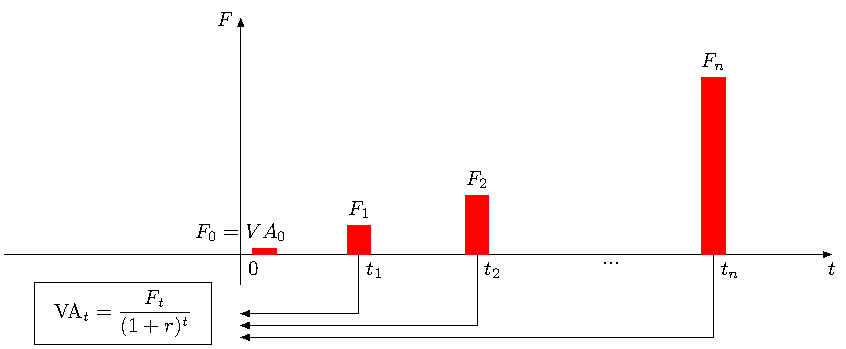
\includegraphics[width=0.7\textwidth]{tikz/attualizzazione.pdf}
    \caption{Operazione di attualizzazione di flussi di cassa futuri}
\end{figure}
\subsection{Criteri di selezione degli investimenti}
\subsubsection{Valore Attuale Netto (VAN)}
È il criterio concettualmente più corretto. Misura la differenza tra il valore attuale dei flussi di cassa futuri ($F_t$) e l'investimento iniziale ($I$). 
\[\textbf{Se VAN>0, l'investimento crea valore}\]
\begin{align*}
     & \text{VAN} = -I + \sum_{t=0}^{n} \frac{F_t}{(1 + r)^t}                                                \\
     & \text{VAN} = -I + \displaystyle \frac{F_1}{(1+r)^1} + \frac{F_2}{(1+r)^2} + ... + \frac{F_n}{(1+r)^n}
\end{align*}
\begin{figure}[H]
    \centering
    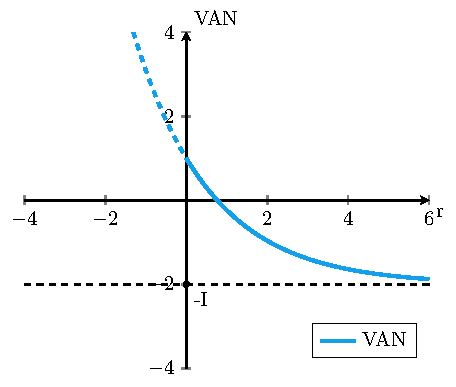
\includegraphics[width=0.4\textwidth]{tikz/van.pdf}
    \caption{Visualizzazione del VAN}
\end{figure}

\subsubsection{Tasso Interno di Rendimento (TIR)}
È il tasso di sconto che rende il VAN pari a zero. Il progetto è accettabile se il TIR è maggiore di  (costo opportunità del capitale). 
Il \textbf{TIR} è quel valore del tasso di attualizzazione  che rende il \textbf{VAN dell'investimento pari a zero}. È un indicatore della redditività di un progetto.
Negli investimenti scelgo il progetto con il TIR maggiore.
\begin{align*}
     & \text{TIR} = \left\{\textcolor{myblue}{r} \quad | \quad \text{VAN} =-  I+ \sum_{t=0}^{n} \frac{F_t}{(1 + \textcolor{myblue}{r})^t} = 0 \right\}                                      \\
\end{align*}
\begin{figure}[H]
    \centering
    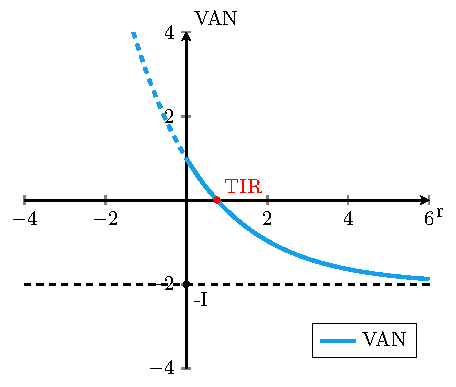
\includegraphics[width=0.4\textwidth]{tikz/tir.pdf}
    \caption{Visualizzazione del TIR}
\end{figure}
\textit{Limitazioni}: Il TIR può essere ambiguo se i flussi di cassa cambiano segno più volte e non è sempre adeguato per confrontare progetti alternativi.

\subsubsection{Tempo di recupero (Payback Period)}
Metodo semplice ma imperfetto che calcola il tempo necessario affinché i flussi di cassa cumulati eguaglino l'esborso iniziale. Il metodo non tiene conto del valore del tempo (attualizzazione) né dei flussi che si manifestano oltre il periodo di recupero.

\subsubsection{Tempo di recupero attualizzato (Payback Period attualizzato)}
Simile al Payback Period, ma considera il valore del tempo attualizzando i flussi di cassa. Ovvero è il periodo necessario affinché il VAN diventi positivo.

\subsubsection{Rendimento Medio Contabile (RMC)}
Il rendimento medio contabile (accountiny rate of return) è un rapporto tra il reddito o utile contabile medio del progetto e il valore contabile netto medio dell'investimento. Questo metodo è debole perché utilizza i valori contabili (reddito) anziché i flussi di cassa e ignora il valore del tempo.
\[ \frac{\text{Utile medio}}{\text{Valore contabile netto medio}} \]
\[\text{Utile medio} = \frac{\text{Utile totale}}{n} \]
\[\text{Valore contabile netto medio} = \frac{\text{Valore contabile iniziale} + \text{Valore contabile finale}}{2} \]

\subsubsection{Rendita perpetua}La rendita perpetua, o \textit{perpetuity}, è una serie di flussi di cassa di uguale importo che si ripetono all'infinito. È un concetto utilizzato in finanza per valutare il valore presente di flussi di cassa che si prevede continueranno in eterno. Tipicamente, si considera in contesti come valutazioni immobiliari (affitti) o titoli finanziari che pagano dividendi costanti.
\[\text{VA} = \frac{F}{r}\]






\subsection{Prospetto dei flussi di cassa}
\subsubsection{Rendiconto dei flussi di cassa differenziale}
Partendo dal bilancio di esercizio, in genere il \textbf{conto economico (a costo del venduto)}, si aggiungono le voci che non hanno effetto sul flusso di cassa e si eliminano le voci che non hanno effetto sul flusso di cassa.
L'analisi di un investimento si deve basare sui flussi di cassa \textbf{differenziali} (incassi o minori esborsi incrementali) che il progetto prospetta, e non sul reddito contabile.
\begin{table}[H]
    \adjustbox{max width=\textwidth,center}{
        \begin{tabular}{|l|V{0.25\textwidth}|c|c|c|c|c|c|}
            \rowcolor{myblue}
            \multicolumn{8}{|c|}{\color{white}\textbf{Prospetto dei flussi di cassa differenziali (5 anni)}} \\
            \hline
            \textbf{Voce} & \textbf{Note} & \textbf{Anno 0} & \textbf{Anno 1} & \textbf{Anno 2} & \textbf{Anno 3} & \textbf{Anno 4} & \textbf{Anno 5} \\
            \hline


            \hline
            \textbf{$+\Delta$ Ricavi} &
            \tiny Incremento dei ricavi/risparmi rispetto allo scenario senza progetto (solo effetti differenziali). &  &  &  &  &  &  \\
            \textbf{$-\Delta$ Costi operativi} &
            \tiny Costi incrementali di competenza (materie, energia, manutenzioni, personale, servizi). &  &  &  &  &  &  \\
            \textbf{$=\Delta$ Margine operativo (EBITDA)} & \tiny Risultato “cash-like” prima di D\&A: misura la performance operativa lorda del progetto. &  &  &  &  &  &  \\
            \hline
            \textbf{$-$ Ammortamenti} & \tiny Quota economica non monetaria del nuovo investimento (costo ripartito nel tempo). &  &  &  &  &  &  \\
            \textbf{$=\Delta$ Risultato operativo (EBIT)} & \tiny Reddito operativo incrementale prima di oneri/proventi finanziari e imposte. &  &  &  &  &  &  \\
            \hline
            \textbf{$-$ Imposte sul reddito} &
            \tiny Imposte calcolate sull’EBIT differenziale con l’aliquota effettiva prevista. &  &  &  &  &  &  \\
            \textbf{$=\Delta$ Utile netto differenziale} &
            \tiny Risultato economico netto del progetto: base di partenza per la conversione in cassa. &  &  &  &  &  &  \\
            \hline
            \rowcolor{myblue}
            \multicolumn{8}{|l|}{\color{white}\textbf{A) Utile differenziale — conto economico incrementale}} \\
            \hline

            \textbf{$+$ Ammortamenti} &
            \tiny Si riaggiungono perché non generano esborso monetario. &  &  &  &  &  &  \\
            \textbf{$\pm$ Plus/minusvalenze da alienazione} & \tiny Voci contabili (prezzo di vendita $-$ valore contabile residuo): si stornano dal cash per evitare doppi conteggi. &  &  &  &  &  &  \\
            \textbf{$=$ Rettifiche non monetarie} & \tiny Totale delle rettifiche non monetarie: \( (B) = + \text{Ammortamenti} \pm \text{Plus/minusvalenze} \). &  &  &  &  &  &  \\
            \hline
            \rowcolor{myblue}
            \multicolumn{8}{|l|}{\color{white}\textbf{B) Rettifica componenti non monetarie}} \\

            \hline
            \textbf{$\pm\,\Delta$ CCN} & \tiny Dilazioni di pagamento a clienti/fornitori e variazioni di magazzino: variazione del capitale circolante netto (CCN). & \textbf{$-$} &  &  &  &  &  \\

            \textbf{= Flusso di cassa operativo (FCO)} &
            \tiny Risultato monetario della gestione caratteristica: \( \text{FCO} = (A) + (B) + (C) \). & &  &  &  &  &  \\
            \hline
            \rowcolor{myblue}
            \multicolumn{8}{|l|}{\color{white}\textbf{C) Rettifica Capitale Circolante Netto (CCN)}} \\
            \hline
            \textbf{$-$ Investimenti in immobilizzazioni} &
            \tiny Uscite per acquisto di impianti/macchinari/asset del progetto (tipicamente Anno 0). & \textbf{$-$} &  &  &  &  &  \\
            \textbf{+ Disinvestimenti / Alienazioni} &
            \tiny Incassi da vendita di asset (es. impianto vecchio) durante l’orizzonte di analisi. & \textbf{+} &  &  &  &  &  \\
            \textbf{+ Recupero CCN / Valore residuo} &
            \tiny Smobilizzo di magazzino/crediti e valore di realizzo residuo del bene a fine progetto. &  &  &  &  &  & \textbf{+} \\

            \textbf{= Flusso di Cassa Netto (FCN)} &
            \tiny Sequenza di flussi totali del progetto per VAN, TIR e PBP: \( \text{FCN} = \text{FCO} + D \). &
             &  &  &  &  &  \\
            \hline
            \rowcolor{myblue}
            \multicolumn{8}{|l|}{\color{white}\textbf{D) Flussi di cassa da investimenti e alienazioni}} \\
            \hline
        \end{tabular}
    }
    \caption{Prospetto dei flussi di cassa differenziali su 5 anni}
\end{table}
La convenienza di un investimento si valuta calcolando il VAN e il TIR sui flussi di cassa netti (FCN) differenziali.



\subsubsection{Dividend Discount Model (DDM)}
Il Dividend Discount Model (DDM) è un metodo di valutazione delle azioni che si basa sull'idea che :
\[\textbf{il valore di un'azione è pari al valore attuale dei dividendi futuri che l'azione genererà}\]
È utile per stabilire il valore dell'\textbf{equity} (Capitale azionario) di un'azienda che distribuisce dividendi regolari.
Si parte dal calcolare il valore di una azione e poi si moltiplica per il numero di azioni in circolazione per ottenere il valore totale dell'equity.
Notare che è molto legato ai temi di costo opportunità del capitale e di rendita perpetua.
\[
    P_0 = \frac{Div_1}{r-g}
\]
Dove: $P_0$ = Prezzo attuale dell'azione, $Div_1$ = Dividendo atteso per il prossimo anno, $r$ = Costo opportunità del capitale, $g$ = Tasso di crescita dei dividendi.
\[
    \text{Equity} = P_0 \times \text{N}_{\text{azioni in circolazione}}
\]
\textit{Limitazioni}: 
Non è adatto per aziende che non distribuiscono dividendi o che hanno flussi di cassa irregolari. Inoltre l'assunto di crescita costante a un tasso $g$ è applicabile solo in certi contesti(aziende mature).

\subsection{Discounted Cash Flow Model (DCFM)}
Il Discounted Cash Flow Model (DCFM) è una evoluzione del DDM che considera i flussi di casssa \textit{unlevered} generati dall'attività dell'azienda come una migliore stima del valore dell'azienda rispetto ai soli dividendi.
\subsubsection{Flusso di cassa unlevered (UCF)}
Nella valutazione non si sottraggono gli interessi passivi dalle entrate, perché gli interessi sono un costo di finanziamento, non un costo operativo. 
Si usa un tasso di attualizzazione, il WACC, che include il costo del debito (e quindi degli interessi) per riflettere il costo totale del capitale.
\subsubsection{Esempio di calcolo di flussi di cassa unlevered}
Nota che è strettamente correlato alla costruzione del prospetto dei flussi di cassa differenziali.
\begin{table}[H]
    \adjustbox{max width=\textwidth,center}{
        \begin{tabular}{|l|V{0.25\textwidth}|c|c|c|c|c|c|}
            \rowcolor{myblue}
            \multicolumn{8}{|c|}{\color{white}\textbf{Prospetto del Flusso di Cassa Unlevered (5 anni)}} \\
            \hline
            \textbf{Voce} & \textbf{Note} & \textbf{Anno 0} & \textbf{Anno 1} & \textbf{Anno 2} & \textbf{Anno 3} & \textbf{Anno 4} & \textbf{Anno 5} \\
            \hline

            \textbf{Ricavi (g=8\%)} &
            \tiny Valore delle vendite generate dalle attività core. Spesso ipotizzato in crescita con tasso $g$. & 1.000 & 1.080 & 1.166 & 1.260 & 1.360 & 1.469 \\
            \hline

            \textbf{EBITDA(36\%)} &
            \tiny Reddito operativo lordo: misura la capacità operativa prima di ammortamenti e accantonamenti. &
             & 389 & 420 & 453 & 490 & 529 \\
            \hline

            \textbf{$-$ Ammortamenti e accantonamenti} &
            \tiny Quote non monetarie di consumo del capitale fisso (non influiscono sul cash flow). &
             & (60) & (60) & (60) & (60) & (60) \\

            \textbf{$=$ EBIT} &
            \tiny Risultato operativo netto di competenza prima delle imposte e degli oneri finanziari. &
             & 329 & 360 & 393 & 430 & 469 \\
            \hline

            \textbf{$-$ Imposte sul reddito} &
            \tiny Imposte calcolate sull’EBIT, al netto del tax rate operativo (es. 28\%). &
             & (92) & (101) & (110) & (120) & (131) \\

            \textbf{$=$ NOPAT (Net Operating Profit After Taxes)} &
            \tiny Net Operating Profit After Taxes: utile operativo dopo le imposte, base del UCF. &
             & 237 & 259 & 283 & 309 & 338 \\
            \hline

            \textbf{$-$ CAPEX (Capital Expenditure)} &
            \tiny Spese per investimenti in attività immobilizzate di natura operativa. &
             & (57) & (62) & (67) & (72) & (78) \\


            \textbf{$\pm \Delta$ CCN (Capitale Circolante Netto)} &
            \tiny Variazioni operative in crediti, debiti e scorte (assorbimento o rilascio di cassa). &
             & (16) & (17) & (19) & (20) & (22) \\


            \textbf{$+$ Ammortamenti} &
            \tiny Riaggiunti poiché non rappresentano uscite di cassa. &
             & 60 & 60 & 60 & 60 & 60 \\


            \textbf{$=$ Flusso di cassa unlevered disponibile(UCF)} &
            \tiny Flusso di cassa operativo \textbf{unlevered}, non considera le variazioni di cassa derivanti da accensioni di debiti. &
             & 224 & 240 & 258 & 279 & 298 \\
            \hline

            \rowcolor{myblue}
            \multicolumn{8}{|l|}{\color{white}\textbf{Valutazione e terminal value}} \\
            \hline

            \textbf{Valore terminale (TV)} &
            \tiny Calcolato come $\text{TV} = \dfrac{\text{UCF}_{5}(1+g)}{\text{WACC} - g}$, rappresenta il \textbf{valore all'anno 5} dei flussi oltre l’anno 5. & & & & & & $6.335$  \\
            \hline

            \textbf{VA Flusso di cassa disponibile (WACC = 6{,}8\%)} &
            \tiny Valore attuale dei flussi scontati al WACC. & 
             & 209 & 211 & 212 & 214 & 4.774 \\
            \hline

            \textbf{Enterprise Value} &
            \tiny Somma dei valori attuali dei UCF e del TV: misura del valore economico complessivo dell’impresa. & \multicolumn{6}{c|}{ $ \frac{224}{(1+0.068)^{1}} + \frac{240}{(1+0.068)^{2}} + \frac{258}{(1+0.068)^{3}} +  \frac{279}{(1+0.068)^{4}} + \frac{(298+6.335)}{(1+0.068)^{5}} = 5.620 $}\\
            \hline
        \end{tabular}
    }
    \caption{Prospetto del flusso di cassa unlevered (UCF) — Valutazione su 5 anni}
\end{table}
\subsubsection{Terminal Value (TV)}
Il Terminal Value (TV) rappresenta il valore all'ultimo anno di previsione dei flussi di cassa futuri oltre il periodo di previsione esplicita, è come una rendita perpetua scontata al costo medio ponderato del capitale (WACC) sottratto il tasso di crescita perpetua ($g$).
Andrà poi attualizzato al momento presente.
\[\text{TV} = \frac{\text{UCF}_{5}(1+g)}{\text{WACC} - g}\]

\subsubsection{Valore attuale del flusso di cassa disponibile (VA)}
Il valore attuale del flusso di cassa disponibile (VA) si ottiene attualizzando i flussi di cassa futuri al costo medio ponderato del capitale (WACC).
\[\text{VA} = \sum_{t=1}^{n} \frac{\text{UCF}_t}{(1 + \text{WACC})^t}\]
\subsubsection{Enterprise Value (EV)}
L'Enterprise Value (EV) rappresenta il valore dell'attivo caratteristico dell'impresa, ossia capitale azionario (equity) più il debito, con cui si finanzia per sostenere la sua operatività. 
\[\text{EV} = \text{VA} + \frac{\text{TV}}{(1+\text{WACC})^n} \]

\textit{Osservazioni}: Il DCFM utilizza il flusso di cassa unlevered (UCF) \textbf{perché poi si sconta al WACC} (Weighted Average Cost of Capital), che riflette il costo complessivo del capitale (sia equity che debito). 
\subsubsection{Capitale Azionario (Equity)}
\begin{table}[H]
    \setlength{\extrarowheight}{12pt} 
    \adjustbox{max width=\textwidth,center}{ 
        \begin{tabular}{|l|c|V{0.25\textwidth}|}
            \rowcolor{myblue}
            \multicolumn{3}{|c|}{\color{white}\textbf{Discounted Cash Flow}} \\
            \hline
            \textbf{Voce}                & \textbf{Formula}                           & \textbf{Note} \\
            \hline
            \textbf{Enterprise Value}    & $\text{EV}= \text{VA} + \displaystyle \frac{\text{TV}}{(1+\text{WACC})^n}$       & \tiny Valore dell'attivo caratteristico dell'impresa, attualizzando i flussi \textit{unlevered} al WACC  \\
            \textbf{Posizione finanziara netta (PFN)} & $\text{PFN} = \text{Debiti} - \text{Liquidità} $ & \tiny Somma algebrica di debiti e attività finanziarie prontamente liquidabili \\
            \textbf{Surplus asset}       & $\text{Surplus asset} $ & \tiny  asset che non sono necessari per la gestione caratteristica, vengono valorizzati al loro valore di mercato \\
            \hline
            \textbf{Capitale Azionario}   & $\text{Equity} = \text{EV}  \pm \text{PFN} + \text{Surplus asset}$ & \tiny Calcolo del capitale azionario (Equity) \\
            \hline
        \end{tabular}
    }
    \caption{Calcolo del capitale azionario (Equity) con DCFM }
\end{table}
\section*{01 Il Valore delle imprese}
Outline completa dei contenuti della lezione:
{\small
\begin{enumerate}
    \item Il valore delle imprese
    \item Obiettivo dell’impresa
    \item Qual è l’obiettivo dell’impresa?
    \item La creazione di valore e gli obiettivi dell’impresa
    \item Il significato di valore (Contabile, Economico, di Mercato)
    \item Valore contabile dell’impresa
    \item Valore economico dell’impresa
    \item Valore contabile e valore economico: due logiche diverse
    \item Il valore di mercato
    \item Valore di liquidazione e avviamento
    \item Calcolo del valore economico di un’impresa
    \item Dividend discount model - 1 (Componenti del ritorno)
    \item Dividend discount model - 2 (Prezzo futuro e formula generale)
    \item Dividend discount model - 3 (Orizzonte infinito e capital gains)
    \item Dividend discount model - 4 (Modello di Gordon)
    \item Discounted cash flow (DCF)
    \item Discounted cash flow: le attività dell’impresa
    \item Discounted cash flow: calcolo del flusso di cassa operativo
    \item Flusso di cassa unlevered: calcolo (EBITDA $\rightarrow$ FCF)
    \item Valutazione Lusso SpA (Esempio numerico)
    \item Esempio di valutazione Lusso SpA: Ipotesi e dati (Capex e CCN)
    \item Valutazione Lusso SpA: Terminal value (TV)
    \item Enterprise Value e valore dei debiti
    \item Valutazione del valore economico dell’azienda (Formula finale)
    \item Per chi si deve creare valore: shareholders o stakeholders?
    \item Shareholder e stakeholder: il dibattito (Diritti espliciti e impliciti)
    \item Obiettivo dell’impresa: Creazione di valore economico per l’azionista
\end{enumerate}
}
\hrule
\vspace{0.5cm}

Buongiorno! Sono felice di iniziare questo percorso con te. Preparare Gestione Aziendale non è solo imparare formule, ma capire la "vita" e la direzione strategica di una realtà complessa come l'impresa. In questa prima lezione ci interroghiamo su un concetto fondamentale: qual è l'obiettivo ultimo di un'impresa?

\subsection*{Dall'illusione del Profitto alla Realtà del Valore}

Tradizionalmente, si è sempre pensato che l'obiettivo fosse la \textbf{massimizzazione del profitto}, ma oggi sappiamo che questo approccio è troppo generico per guidare davvero il comportamento aziendale. Il profitto è un dato contabile soggetto a molte interpretazioni: ad esempio, capitalizzare un costo invece di spesarlo aumenta i profitti di breve periodo ma riduce quelli di lungo. Per questo motivo, la bussola del management si è spostata sulla \textbf{creazione di valore}.

Ma cosa intendiamo esattamente per "valore"? In azienda non esiste un'unica definizione, ma dobbiamo saper navigare tra tre accezioni diverse e complementari:

\begin{table}[H]
    \setlength{\extrarowheight}{12pt}
    \adjustbox{max width=\textwidth,center}{
        \centering
        \begin{tabular}{|l|V{0.35\textwidth}|V{0.35\textwidth}|}
            \hline
            \rowcolor{myblue}
            \textbf{Tipologia di Valore} & \textbf{Logica Sottostante} & \textbf{Significato Pratico} \\
            \hline
            \textbf{Valore Contabile} & 
            \small \textbf{Quanto denaro è stato investito?} Deriva dallo Stato Patrimoniale (Capitale Netto) e segue principi di prudenza e costi storici. & 
            \small È un dato "povero" e storico; non riflette il potenziale futuro né le risorse intangibili come la reputazione o la tecnologia. \\
            \hline
            \textbf{Valore Economico} & 
            \small \textbf{Quali benefici trarremo in futuro?} Si basa sull'attualizzazione dei flussi di cassa futuri attesi. & 
            \small Dipende dalla redditività attesa e dal rischio (costo opportunità del capitale). \\
            \hline
            \textbf{Valore di Mercato} & 
            \small \textbf{A che prezzo avviene lo scambio?} È il prezzo di equilibrio tra domanda e offerta sui mercati. & 
            \small Coincide con il valore economico solo se i mercati sono efficienti. \\
            \hline
        \end{tabular}
    }
    \caption{Tipologie di valore d'impresa}
\end{table}

\subsection*{La Logica del Valore Economico: Perché la Cassa e non l'Utile?}

È qui che molti studenti si confondono, ma seguimi bene: la teoria finanziaria preferisce i \textbf{flussi di cassa} (Cash Flows) ai ricavi o ai costi economici. Il motivo è logico: un ricavo (fatturato) non è un'entrata immediata di denaro se vendo a credito. Per valutare un investimento, dobbiamo guardare al "soldo" che entra ed esce realmente, perché è quello che determina la capacità dell'impresa di sopravvivere e remunerare i suoi finanziatori.

Per trasformare questi flussi futuri in un valore odierno, usiamo il \textbf{tasso di attualizzazione}, ovvero il \textbf{costo opportunità del capitale}. Questo rappresenta la soglia minima di rendimento che un investitore si aspetta per rinunciare a investimenti alternativi con lo stesso grado di rischio.

\subsection*{Il Valore tra Funzionamento, Liquidazione e Avviamento}

Dobbiamo anche distinguere tra il valore dell'impresa "viva" e quello "morta". Il \textbf{Valore di Funzionamento} considera l'impresa come un sistema coordinato capace di produrre ricchezza, mentre il \textbf{Valore di Liquidazione} è ciò che si ottiene vendendola "a pezzi". La differenza tra questi due è l'\textbf{avviamento} (Goodwill), che rappresenta il valore intangibile (reputazione, know-how, marchi) che rende il tutto superiore alla somma delle singole parti.

\subsection*{Modelli di Calcolo: DDM e DCF}

Per calcolare il valore economico, abbiamo due strade principali:

\begin{enumerate}
\item \textbf{Dividend Discount Model (DDM):} vede il valore dell'azione come il valore attuale dei dividendi futuri attesi. Se immaginiamo di detenere l'azione all'infinito, i guadagni in conto capitale (capital gains) spariscono dalla formula perché proiettati troppo lontano. Una formula celebre è quella di \textbf{Gordon}, che ipotizza una crescita costante ($g$) dei dividendi all'infinito: $P_0 = Div_1 / (r - g)$.

\item \textbf{Discounted Cash Flow (DCF):} è l'evoluzione del DDM usata nella pratica aziendale. Invece di stimare i dividendi (che l'azienda potrebbe decidere di non distribuire), stimiamo i \textbf{flussi di cassa disponibili} generati dall'attività operativa.

\end{enumerate}

Abbiamo capito che il profitto contabile è un'illusione manovrabile; la realtà è il valore economico, e per calcolarlo la finanza ci offre due modelli fondamentali che ora analizzeremo nel dettaglio.

\subsection*{Il Dividend Discount Model (DDM): L'illusione dei Capital Gains}

Il DDM è il punto di partenza teorico. Immaginiamo di possedere un'azione: da dove arriva il nostro guadagno? Da due fonti: il \textbf{dividendo} (la cedola annuale) e il \textbf{capital gain} (l'aumento di prezzo del titolo). 
Il rendimento percentuale atteso ($r$) si esprime così:
\[ r = \frac{Div_1 + (P_1 - P_0)}{P_0} \]
Se invertiamo la formula per trovare il prezzo oggi ($P_0$), scopriamo che il valore di un'azione è il valore attuale del dividendo dell'anno prossimo più il prezzo a cui pensiamo di rivenderla:
\[ P_0 = \frac{Div_1}{1+r} + \frac{P_1}{1+r} \]
Ma cosa determina $P_1$? Lo stesso ragionamento: i dividendi dell'anno 2 e il prezzo $P_2$. Se proseguiamo questo processo all'infinito ($H \rightarrow \infty$), il prezzo finale $P_H$ tende a zero nel calcolo del valore attuale, e i capital gains "spariscono" dalla formula. Il valore dell'azione oggi è semplicemente la sommatoria di tutti i dividendi futuri attualizzati. 

Per rendere questo calcolo pratico, usiamo il \textbf{Modello di Gordon}, che ipotizza una crescita costante ($g$) dei dividendi all'infinito:
\[ P_0 = \frac{Div_1}{r - g} \]
Qui capiamo un concetto logico fondamentale: un'azienda vale di più se distribuisce dividendi alti ($Div_1$), se cresce molto ($g$), o se è poco rischiosa (basso $r$).

\subsection*{Dal DDM al Discounted Cash Flow (DCF): La centralità della Cassa}

Nella pratica aziendale, il DDM ha un limite: molte aziende non distribuiscono dividendi pur creando valore (pensa a Google o alle startup). L'evoluzione è il \textbf{Discounted Cash Flow (DCF)}, che sostituisce i dividendi con i \textbf{Flussi di Cassa Disponibili (Free Cash Flows)}. Il principio è: il dividendo è solo una scelta di distribuzione, ma il valore è generato dalla capacità dell'impresa di produrre "soldo" reale.



\subsection*{Il Caso Lusso SpA: Mettere i numeri a sistema}

L'esempio della \textbf{Lusso SpA} ci mostra come si valuta un'azienda "viva". Il processo avviene in due stadi:
\begin{enumerate}
    \item \textbf{Primo stadio (Previsione esplicita):} Per 5 anni stimiamo i flussi anno per anno. Notiamo che se il fatturato cresce (ipotesi 8\%), dobbiamo investire in \textbf{CAPEX} (macchinari) e \textbf{CCN} (crediti e scorte). Più l'azienda cresce velocemente, più cassa "mangia" nel breve termine.
    \item \textbf{Secondo stadio (Valore Finale - TV):} Poiché non possiamo prevedere il dettaglio per sempre, ipotizziamo che dal sesto anno l'azienda cresca a un tasso stabile (es. 2\%). Calcoliamo il \textbf{Terminal Value} attualizzando questa rendita perpetua:
    \[ TV_5 = \frac{FCF_6}{WACC - g} \]
\end{enumerate}
Attualizzando i flussi dei primi 5 anni e il Terminal Value al costo del capitale (\textbf{WACC} 6.8\%), otteniamo l'\textbf{Enterprise Value} di 5.620.

\subsection*{Enterprise Value e la Formula Finale del Valore}

Attenzione alla distinzione cruciale: quello che abbiamo calcolato finora è l'\textbf{Enterprise Value (EV)}, ovvero il valore di tutte le attività operative (il core business). Ma noi vogliamo sapere quanto valgono le azioni (\textbf{Equity}).
L'azionista è un \textbf{soggetto residuale}: prende quello che resta dopo aver pagato i debiti.

La formula per la \textbf{Valutazione del valore economico dell'azienda (Equity Value)} è:
\[
\textbf{Valore Equity} = \textbf{Enterprise Value} \pm \textbf{Posizione Finanziaria Netta (PFN)} + \textbf{Surplus Assets}
\]

\begin{itemize}
    \item \textbf{PFN (Posizione Finanziaria Netta):} È la differenza tra i debiti finanziari e la liquidità (cassa e titoli). Se l'azienda ha più debiti che cassa, la PFN si sottrae all'EV.
    \item \textbf{Surplus Assets:} Sono attività non necessarie alla gestione operativa (es. un quadro di valore, un terreno non usato). Vengono aggiunti al valore perché potrebbero essere venduti senza danneggiare il core business.
\end{itemize}

In conclusione, caro studente, ricorda la logica: partiamo dai flussi di cassa operativi, li attualizziamo per trovare il valore del "motore" dell'azienda (Enterprise Value), e poi aggiungiamo la benzina avanzata (cassa) e sottraiamo i debiti per capire quanto resta in tasca all'azionista. 



\subsection*{Shareholder o Stakeholder? Per chi creiamo valore?}

Il dibattito è storico. \textbf{Milton Friedman} sosteneva che l'unico obiettivo fosse il valore per gli azionisti (\textit{shareholders}). \textbf{Edward Freeman}, invece, ha introdotto la teoria degli \textit{stakeholders}, sostenendo che l'impresa deve creare valore per tutti i portatori d'interesse (dipendenti, fornitori, comunità, ambiente).

Oggi la sintesi è chiara: l'obiettivo è la creazione di valore per l'azionista nel \textbf{lungo termine}, ma questo è possibile solo se si soddisfano le aspettative degli altri stakeholders. Se tradisci i dipendenti o inquini l'ambiente, distruggi il \textbf{capitale reputazionale}, e questo farà crollare il valore economico per l'azionista stesso. Il diritto dell'azionista è un \textbf{diritto residuale}: riceve ciò che resta solo dopo aver pagato tutti gli altri.

In sintesi, il tuo compito come futuro manager sarà agire sulle leve di lungo termine per accrescere il valore economico, assicurando che il rendimento dei tuoi investimenti sia sempre superiore al costo del capitale.

Ti è tutto chiaro su questo primo mattone logico? Se sì, siamo pronti a passare ai "fondamentali" del valore!

\section*{02 Il Valore delle imprese}

Outline completa dei contenuti della lezione:
{\small
\begin{enumerate}
\item I fondamentali del valore
\item Redditività del capitale investito e costo del capitale
\item Redditività del capitale investito (ROI)
\item Redditività del capitale investito – Le 2 variabili chiave: la redditività delle vendite (ROS) e la rotazione del capitale investito (AT)
\item Il costo del capitale
\item WACC - Weighted Average Cost of Capital (Costo medio ponderato del capitale)
\item Calcolo del WACC – Impresa Lusso SpA
\item WACC (1) - Capital Asset Pricing Model (CAPM)
\item WACC (2) - Capital Asset Pricing Model (CAPM): Dati per Lusso SpA
\item WACC (3): Struttura finanziaria di settore
\item WACC (4): Calcolo finale per Lusso SpA
\item Il value based management (VBM)
\item Flussi di cassa e valore
\item Creazione di valore: relazione tra redditività del capitale investito, investimenti e flussi di cassa
\item Analisi comparativa: Impresa 1 (Crescita 5\%, ROI 20\%)
\item Analisi comparativa: Impresa 2 (Crescita 5\%, ROI 10\%)
\item Analisi comparativa: Impresa 3 (Crescita 8\%, ROI 20\%)
\end{enumerate}
}
\hrule
\vspace{0.5cm}

Ben ritrovato! Dopo aver definito nella prima lezione cosa sia il valore, oggi entriamo nel "motore" dell'impresa per analizzarne i \textbf{fondamentali}. Non basta generare cassa: per capire se un'azienda sta davvero prosperando, dobbiamo mettere in relazione quanto rende il capitale investito con quanto costa quel capitale agli investitori.

\subsection*{La Sfida Centrale: Redditività vs Costo del Capitale}

Il concetto cardine della gestione aziendale moderna è la sfida tra due percentuali: la \textbf{redditività del capitale investito} e il \textbf{costo del capitale}.
\begin{itemize}
    \item \textbf{Generazione di valore:} si verifica se l'azienda genera una redditività superiore al costo del capitale, portando a un Valore Attuale Netto (VAN) maggiore di zero.
    \item \textbf{Distruzione di valore:} avviene se la redditività è inferiore al costo del capitale. In questo caso, anche se l'azienda produce utili contabili, sta "mangiando" la ricchezza degli investitori perché non remunera adeguatamente il rischio (VAN < 0).
\end{itemize}

\subsection*{Misurare la Redditività: Il Modello DuPont}

Per misurare la redditività del capitale investito utilizziamo il \textbf{ROI (Return On Investment)}, calcolato come rapporto tra Reddito Operativo (Ebit) e Capitale Investito (Attività). Per capire come migliorare questo indice, facciamo ricorso al celebre \textbf{Modello DuPont}, che scompone il ROI in due variabili operative:

\begin{table}[H]
\setlength{\extrarowheight}{10pt}
\adjustbox{max width=\textwidth,center}{
\centering
\begin{tabular}{|l|c|V{0.45\textwidth}|}
\hline
\rowcolor{myblue}
\textbf{Variabile} & \textbf{Formula} & \textbf{Significato Manageriale} \\
\hline
\textbf{ROS (Return On Sales)} & $RO / S$ & Misura la redditività delle vendite, ovvero quanto margine resta per ogni euro di fatturato. \\
\hline
\textbf{AT (Asset Turnover)} & $S / A$ & Misura la rotazione del capitale, ovvero l'efficienza con cui l'impresa usa le proprie attività per generare vendite. \\
\hline
\end{tabular}
}
\caption{Scomposizione del ROI secondo il sistema DuPont}
\end{table}

Managerialmente, lo stesso ROI può essere ottenuto con strategie opposte: puntando su \textbf{alti margini} (tipico del lusso, con bassa rotazione) o sulla \textbf{velocità di rotazione} (tipico della grande distribuzione, con bassi margini). L'efficienza non dipende solo dal volume, ma dalla capacità del capitale investito di fare leva sulla produzione di profitto.

\subsection*{Il Costo del Capitale: L'Asticella del Valore}

Il costo del capitale rappresenta la \textbf{soglia minima di rendimento} attesa dagli investitori (azionisti e creditori) per le risorse fornite. È un \textbf{costo opportunità}: l'investitore rinuncia a investimenti alternativi con lo stesso grado di rischio per scommettere sulla tua impresa.

Per quantificare questa soglia utilizziamo il \textbf{WACC (Weighted Average Cost of Capital)}, che è la media ponderata tra il costo del Capitale Proprio ($r_e$) e il costo del Debito ($r_d$), quest'ultimo calcolato al netto delle imposte ($T_c$) poiché gli interessi passivi sono deducibili.
\[ WACC = r_e \frac{E}{D+E} + r_d (1 - T_c) \frac{D}{D+E} \]

Per stimare il costo dell'equity ($r_e$), utilizziamo il \textbf{CAPM (Capital Asset Pricing Model)}, dove il \textbf{Beta} ($\beta$) misura il rischio sistematico del settore.
Nel caso di \textbf{Lusso SpA}, con un $\beta$ di 0.99, un tasso risk-free del 2.76\% e un premio per il rischio di mercato del 6.5\%, il costo dell'equity risulta del 9.2\%. Integrando un costo del debito del 4.5\% e un'aliquota fiscale del 24\%, otteniamo un WACC finale del \textbf{6.8\%}.

\subsection*{Il Valore della Crescita: Analisi di Tre Imprese}

Una delle lezioni più importanti riguarda il legame tra crescita, investimenti e valore. Analizziamo tre imprese con lo stesso reddito iniziale (100) e lo stesso costo del capitale (10\%):

\begin{itemize}
    \item \textbf{Impresa 1 (ROI 20\%, Crescita 5\%):} Investe il 25\% del reddito. Avendo una redditività superiore al costo del capitale, il suo valore economico (1.500) supera quello contabile (1.000). \textbf{Crea valore}.
    \item \textbf{Impresa 2 (ROI 10\%, Crescita 5\%):} Investe il 50\% del reddito. Nonostante investa il doppio della prima, il suo ROI è uguale al costo del capitale. Il valore dell'impresa resta identico a quello contabile (1.000). \textbf{Investire senza efficienza non serve a nulla}.
    \item \textbf{Impresa 3 (ROI 20\%, Crescita 8\%):} Investe il 40\% del reddito. Rinuncia a flussi di cassa nel breve termine per finanziare una crescita maggiore (8\%) con investimenti efficaci. Il suo valore esplode a \textbf{3.000}.
\end{itemize}

\subsection*{Value Based Management (VBM)}

Spesso le imprese trascurano il calcolo del costo del capitale perché non è richiesto dai bilanci obbligatori. Tuttavia, ignorarlo è pericoloso: si rischia di identificare il costo del capitale con il solo costo del debito (che è sempre inferiore) o di finanziare progetti che distruggono ricchezza. Il \textbf{Value Based Management} consiste nell'introdurre strumenti che monitorino costantemente la creazione di valore economico, assicurando che ogni decisione operativa sia volta all'incremento del valore nel lungo periodo.

Ti è chiaro come l'efficacia degli investimenti pesi molto più della loro semplice entità numerica? Se sei pronto, nella prossima lezione vedremo come il management agisce operativamente per massimizzare questi fondamentali!
\section*{03 Il Valore delle imprese: Priorità Manageriali e Struttura Finanziaria}

Outline completa dei contenuti della lezione:
{\small
\begin{enumerate}
\item Le priorità manageriali per la creazione del valore
\item Rafforzamento del core business e disinvestimento degli asset non strategici
\item Management Buy-out e Spin-off
\item Società di investimento: Private Equity e Venture Capital
\item Il mercato tecnologico: NASDAQ
\item La Teoria dell'Agenzia: relazioni tra proprietà e controllo
\item Sistemi di incentivo: Stock Options e relativi rischi
\item Soluzioni ai costi di agenzia (Corporate Governance e controlli)
\item Uso della leva finanziaria: il teorema di Modigliani-Miller
\item Scelta tra debito ed equity: benefici fiscali e flessibilità
\end{enumerate}
}
\hrule
\vspace{0.5cm}

Bentornato! Se nelle scorse lezioni abbiamo analizzato i numeri (ROI, WACC e flussi di cassa), oggi ci spostiamo su un piano più strategico e comportamentale. Una volta capito come si misura il valore, dobbiamo chiederci: cosa deve fare concretamente il manager per "muovere" quei numeri e far crescere l'azienda?. In questa lezione analizzeremo le leve operative e finanziarie che la direzione deve azionare per non tradire il suo mandato: la creazione di valore nel lungo termine.

\subsection*{Le Priorità Manageriali: Focalizzazione e Pulizia del Portafoglio}

Il primo compito della direzione è favorire processi decisionali che accrescano il valore economico agendo su leve di lungo periodo. Le priorità fondamentali includono:
\begin{itemize}
    \item \textbf{Efficienza e Innovazione:} Focalizzarsi sul miglioramento dei processi e sulla capacità di rinnovare l'offerta.
    \item \textbf{Rafforzamento del Core Business:} Concentrare le risorse sulle attività in cui l'impresa ha un vantaggio competitivo distintivo.
    \item \textbf{Disinvestimento di Asset non Strategici:} Spesso creare valore non significa aggiungere, ma togliere. È necessario dismettere rami d'azienda, divisioni o sedi estere che hanno perso rilevanza strategica.
\end{itemize}

Per attuare questi disinvestimenti, si ricorre spesso a due strumenti tecnici:
\begin{enumerate}
    \item \textbf{Management Buy-out (MBO):} Operazione in cui il management dell'azienda stessa, spesso supportato da fondi di private equity, acquista l'impresa o una sua parte per gestirla in autonomia.
    \item \textbf{Spin-off:} Una divisione o unità organizzativa viene scorporata dalla società madre e resa un'entità indipendente. In ambito accademico, gli spin-off sono essenziali per trasformare la ricerca tecnologica in realtà produttive.
\end{enumerate}

\subsection*{Il Ruolo dei Capitali Esterni: Private Equity e NASDAQ}

Per sostenere la crescita, le imprese ricorrono a società di investimento specializzate nel forniere capitale di rischio:
\begin{itemize}
    \item \textbf{Private Equity:} Investitori che entrano nel capitale di aziende già formate per ristrutturarle e migliorarne la performance.
    \item \textbf{Venture Capital:} Fondi destinati a imprese appena nate (startup) ad alto rischio ma con potenziale tecnologico elevato.
\end{itemize}

Il luogo d'elezione per queste realtà tecnologiche è spesso il \textbf{NASDAQ}, il primo mercato al mondo esclusivamente elettronico, che ospita migliaia di società con elevati tassi di innovazione.

\subsection*{La Teoria dell'Agenzia: Allineare Manager e Azionisti}

Uno dei problemi più complessi della gestione aziendale è il conflitto tra chi possiede l'azienda (\textbf{principals}, gli azionisti) e chi la gestisce (\textbf{agents}, i manager). Spesso i manager hanno obiettivi propri (come la crescita della dimensione aziendale per aumentare il proprio potere) che divergono dalla massimizzazione della ricchezza degli azionisti.

Per ridurre questi "costi di agenzia", le imprese strutturano sistemi premianti:
\begin{table}[H]
\setlength{\extrarowheight}{10pt}
\adjustbox{max width=\textwidth,center}{
\centering
\begin{tabular}{|l|V{0.35\textwidth}|V{0.35\textwidth}|}
\hline
\rowcolor{myblue}
\textbf{Strumento} & \textbf{Meccanismo} & \textbf{Rischi Potenziali} \\
\hline
\textbf{Stock Options} & Diritto di acquistare azioni a un prezzo fisso (striking price). Se il valore dell'azienda sale, il manager guadagna. & \small Ricerca eccessiva del rischio, comportamenti fraudolenti (manipolazione bilanci) o premi basati sul mercato generale invece che sulla bravura reale. \\
\hline
\textbf{Controlli Interni} & Il Consiglio di Amministrazione (CdA) e i codici di autodisciplina vigilano sull'operato manageriale. & \small Bassa indipendenza dei consiglieri o asimmetria informativa tra manager e CdA. \\
\hline
\textbf{Mercato del Controllo} & La minaccia di "scalate ostili" (takeover) da parte di predatori costringe i manager a essere efficienti. & \small Possibile focus eccessivo sul breve termine per evitare cali di borsa. \\
\hline
\end{tabular}
}
\caption{Incentivi e monitoraggio nella Corporate Governance}
\end{table}

\subsection*{La Leva Finanziaria: Debito vs Equity}

L'ultimo driver fondamentale è la struttura finanziaria. Secondo gli studi di \textbf{Modigliani e Miller}, in un mondo ideale il mix tra debito ed equity non influenzerebbe il valore dell'impresa. Tuttavia, nella realtà esistono i **benefici fiscali**: gli interessi sul debito sono deducibili, rendendo l'indebitamento conveniente sotto il profilo fiscale.

Dobbiamo però scegliere con prudenza tra debito ed equity in base alla natura dell'impresa:
\begin{itemize}
    \item \textbf{Debito:} Consigliato per aziende con flussi di cassa stabili, in settori maturi e con bassa incertezza (es. immobiliari).
    \item \textbf{Equity:} Necessario per aziende con elevata incertezza tecnologica o mercati non consolidati (startup), dove serve flessibilità finanziaria che il debito, per sua natura rigido, non può dare.
\end{itemize}

In sintesi, caro studente, ricorda che il manager deve agire come se l'azienda fosse propria, ma con la consapevolezza che il suo diritto è \textbf{residuale}. Solo se soddisfa le aspettative degli stakeholder (clienti, dipendenti, fornitori) riuscirà a creare quel capitale reputazionale che genera valore reale per l'azionista nel lungo termine.
\section*{04 Strategia d'impresa}

Outline completa dei contenuti della lezione:
{\small
\begin{enumerate}
\item La strategia di impresa
\item La strategia - Fattori esterni e fattori interni
\item La strategia - fattori interni e fattori esterni (Strategic Fit)
\item I percorsi che portano alla strategia (Planning, Thinking, Opportunistic)
\item Definizione del Business - Il punto di partenza della strategia (Abell)
\item Il punto di partenza della strategia: la definizione del business
\item Definizione dei gruppi/segmenti di clienti (criteri di identità)
\item L’analisi dei fattori esterni all’impresa e le cinque forze competitive
\item Il Modello di Concorrenza Allargata: le 5 forze competitive (M. Porter)
\item 1. Intensità della concorrenza tra imprese
\item 2. Potenziali entranti: barriere all’entrata
\item 3. Prodotti e servizi sostitutivi
\item 4. Potere contrattuale dei clienti
\item 5. Potere contrattuale dei fornitori
\item Critiche al modello delle forze competitive
\item L’analisi dei fattori interni all’impresa
\item La catena del valore dell’impresa
\item Attività generatrici di valore (Primarie e di Supporto)
\item I legami all’interno della catena del valore
\end{enumerate}
}
\hrule
\vspace{0.5cm}

Benvenuto a questa quarta lezione! Dopo aver capito come si misura il valore di un'impresa, ora dobbiamo chiederci: come si progetta il successo per crearlo davvero? Entriamo nel cuore pulsante della **Strategia d'impresa**. La strategia non è un semplice piano operativo, ma l'insieme integrato di decisioni volte a costruire un vantaggio competitivo che sia difendibile e sostenibile nel lungo periodo.

\subsection*{Il Concetto di "Strategic Fit": L'Equilibrio Perfetto}

Il segreto di una strategia vincente risiede nella coerenza, che noi chiamiamo **Strategic Fit**. Non puoi decidere cosa fare senza guardare contemporaneamente in due direzioni:
\begin{itemize}
    \item \textbf{Analisi Esterna (Environmental Model):} Studia il mercato per individuare opportunità e minacce. Ci dice "cosa il mercato vuole" e come il settore condiziona l'impresa.
    \item \textbf{Analisi Interna (Resource-Based Model):} Guarda dentro l'azienda per mappare forze e debolezze. Si focalizza sulle risorse scarse e sulle competenze uniche che ci differenziano dai competitor.
\end{itemize}
La strategia è il ponte che unisce queste due sponde.

\subsection*{I Percorsi verso la Strategia}

Le imprese non arrivano alla strategia tutte nello stesso modo. Esistono tre percorsi principali:
\begin{enumerate}
    \item \textbf{Strategic Planning:} Un approccio razionale e strutturato che analizza i dati per definire la rotta.
    \item \textbf{Strategic Thinking:} Basato sulla creatività imprenditoriale e sull'intuizione. È il "guizzo" che vede ciò che gli altri non vedono.
    \item \textbf{Opportunistic Decision Making:} La capacità di rispondere in modo efficace a problemi inattesi o opportunità improvvise del mercato.
\end{enumerate}

\subsection*{Definire il Business: Chi, Cosa e Come?}

Prima di combattere, devi sapere in quale campo stai giocando. Per definire il business utilizziamo lo schema di Abell, che si basa su tre dimensioni fondamentali:
\begin{enumerate}
    \item \textbf{Chi stiamo servendo? (Gruppi di clienti):} Non tutto il mercato è uguale. Dobbiamo segmentarlo usando criteri geografici, demografici, socio-economici o psicografici (stili di vita).
    \item \textbf{Quale bisogno soddisfiamo? (Funzioni svolte):} Il cliente non compra un prodotto, ma la soluzione a un bisogno.
    \item \textbf{In che modo lo facciamo? (Modalità):} Quali tecnologie o processi alternativi utilizziamo per rispondere a quel bisogno?.
\end{enumerate}

\subsection*{Il Modello di Porter: Le 5 Forze Competitive}

Per capire quanto sia attrattivo un settore, Michael Porter ci ha regalato uno strumento potentissimo: il **Modello della Concorrenza Allargata**. La redditività di un'impresa non dipende solo dai concorrenti diretti, ma dall'interazione di 5 forze:

\begin{enumerate}
    \item \textbf{Intensità della concorrenza tra imprese esistenti:} Se ci sono troppi attori, la guerra dei prezzi distrugge i margini. Fattori come l'alta presenza di costi fissi o barriere all'uscita elevate (difficoltà a disinvestire impianti specializzati) rendono la lotta più feroce.
    \item \textbf{Minaccia di nuovi entranti:} Quanto è facile per un nuovo nemico entrare nel settore? Questo dipende dalle **barriere all'entrata**, come il fabbisogno di ingenti capitali, le economie di scala (costi più bassi per chi produce già in grandi volumi) o la forte fedeltà dei clienti verso i brand esistenti.
    \item \textbf{Minaccia di prodotti sostitutivi:} Sono prodotti che soddisfano lo stesso bisogno con modalità diverse (es. lo zucchero e il dolcificante). Se il rapporto qualità/prezzo del sostituto è alto e i costi di riconversione per il cliente sono bassi, il settore è a rischio.
    \item \textbf{Potere contrattuale dei clienti:} Se i clienti sono pochi e concentrati, o se acquistano grandi volumi, possono imporre prezzi bassi e sconti.
    \item \textbf{Potere contrattuale dei fornitori:} Specularmente, se i fornitori sono pochi e il loro input è fondamentale e difficile da sostituire, saranno loro a comandare sui margini dell'impresa.
\end{enumerate}

\subsection*{Analisi Interna e la Catena del Valore}

Se l'analisi esterna ci dice quanto il "mare" è tempestoso, l'analisi interna ci dice quanto è robusta la nostra "nave". Lo strumento principale qui è la **Catena del Valore** di Porter, che disaggrega l'impresa in attività strategicamente rilevanti per capire dove si genera davvero il valore:

\begin{itemize}
    \item \textbf{Attività Primarie:} Creano fisicamente il prodotto e lo portano al cliente. Includono la logistica in entrata, le \textit{operations} (produzione), la logistica in uscita, il marketing/vendite e i servizi post-vendita.
    \item \textbf{Attività di Supporto:} Aumentano l'efficienza delle primarie. Sono l'infrastruttura dell'impresa, la gestione delle risorse umane, lo sviluppo della tecnologia (R\&S) e gli approvvigionamenti.
\end{itemize}

Il vero vantaggio competitivo spesso non nasce da una singola attività, ma dai **legami** tra esse. Ad esempio, una progettazione del prodotto più costosa e accurata (Sviluppo tecnologia) può ridurre drasticamente le richieste di assistenza in garanzia (Servizi), creando un vantaggio di ottimizzazione complessiva.

Ricorda sempre, caro studente: l'obiettivo finale è capire se le tue risorse e competenze ti permettono di presidiare i **Fattori Critici di Successo** (FCS) del mercato meglio dei tuoi rivali. Se non è così, la strategia deve cambiare rotta!
\section*{05 Strategia d'impresa}

Outline completa dei contenuti della lezione:
{\small
\begin{enumerate}
\item Il vantaggio competitivo
\item Vantaggio di costo
\item Vantaggio di costo: le determinanti del vantaggio di costo
\item Economie di scala
\item Vantaggio di costo: requisiti in termini di risorse e competenze
\item Vantaggio di costo: con riferimento alla catena del valore
\item Vantaggio di costo: attraverso la riconfigurazione della catena del valore
\item Il vantaggio di costo (riferito alla trasformazione della catena del valore)
\item Vantaggio di differenziazione
\item Vantaggio di differenziazione: requisiti in termini di risorse e competenze
\item Vantaggio di differenziazione: con riferimento alla catena del valore
\item Vantaggio di differenziazione (riferito all'incremento del margine)
\item Swot analysis
\item «Swot analysis» (riferito allo schema grafico)
\end{enumerate}
}
\hrule
\vspace{0.5cm}

Benvenuto! Oggi facciamo un passo avanti decisivo: dopo aver mappato le attività aziendali con la catena del valore, dobbiamo capire come usarle per battere la concorrenza. La strategia non è altro che la scelta del modo in cui l'impresa decide di "vincere" nel proprio mercato, costruendo quello che chiamiamo \textbf{Vantaggio Competitivo}. Esistono due strade maestre, diverse e quasi sempre alternative: la leadership di costo e la differenziazione.

\subsection*{1. La Leadership di Costo: L'Efficienza come Arma}

Un'impresa possiede un vantaggio di costo quando è capace di realizzare tutte le attività della sua catena del valore a un costo totale inferiore rispetto a quello dei concorrenti. Esempi classici che vedi tutti i giorni sono IKEA o Wal-Mart. Ma come si ottiene concretamente questa riduzione? Dobbiamo agire su quelle che chiamiamo \textbf{determinanti di costo}:

\begin{itemize}
    \item \textbf{Economie di scala:} Sono la riduzione dei costi unitari che ottieni aumentando il volume della produzione. Se produci di più, i costi fissi si spalmano su più unità, il tuo potere contrattuale verso i fornitori aumenta e i rischi si riducono. Inoltre, molte attività come la pubblicità o la R\&S non crescono proporzionalmente agli input, rendendo la grande dimensione un enorme vantaggio.
    \item \textbf{Economie di apprendimento:} Più fai una cosa, più impari a farla bene e velocemente, riducendo gli sprechi.
    \item \textbf{Tecnologia e Progettazione:} Innovare il processo produttivo o progettare un prodotto più semplice da montare può abbattere drasticamente i costi.
\end{itemize}

Per gestire questa strategia, l'impresa deve avere una cultura ferrea del controllo: supervisione stretta, reporting frequente, obiettivi quantitativi e incentivi legati ai risparmi. A livello di catena del valore, l'impresa può decidere di \textbf{riconfigurare} tutto il sistema: ad esempio esternalizzando (outsourcing) le attività non critiche, razionalizzando gli stabilimenti o integrandosi verticalmente per eliminare i margini dei fornitori. In questo modo, la catena del valore si "abbassa" e il margine di profitto si espande grazie al minor costo.

\subsection*{2. Il Vantaggio di Differenziazione: L'Unicità che Incanta}

Se non vuoi (o non puoi) essere il più economico, devi essere \textbf{unico}. La differenziazione consiste nel fornire un prodotto o servizio che i clienti percepiscono come superiore, tanto da essere disposti a pagare un \textbf{premium price} (un differenziale di prezzo) che superi i costi aggiuntivi sostenuti per crearlo. Pensa ad Apple o Illy: non sono i più economici, ma sono desiderati per la loro unicità.

I requisiti per questa strategia sono opposti alla precedente:
\begin{itemize}
    \item Servono forti competenze di marketing e ricerca tecnologica d'avanguardia.
    \item Bisogna puntare sull'innovazione di prodotto e sulla qualità assoluta.
    \item È fondamentale attrarre forza lavoro altamente qualificata e motivata.
\end{itemize}

Nella catena del valore, non guardiamo più solo a noi stessi, ma cerchiamo il collegamento con la catena del valore del cliente. Dobbiamo capire quali variabili hanno il maggior potenziale di differenziazione: magari un servizio post-vendita incredibile o un design unico. Qui la catena del valore non si "abbassa", ma si "alza" verso l'alto: aumentano i costi per dare più qualità, ma i ricavi crescono molto di più, espandendo comunque il margine finale.

\subsection*{3. La Sintesi Perfetta: SWOT Analysis}

Per decidere quale di queste due strade prendere, il manager ha bisogno di una bussola: la \textbf{SWOT Analysis}. È uno schema grafico che mette insieme tutto quello che abbiamo studiato:
\begin{enumerate}
    \item \textbf{Ambiente Interno:} Mappiamo le nostre \textbf{Forze} (Strengths) e \textbf{Debolezze} (Weaknesses).
    \item \textbf{Ambiente Esterno:} Identifichiamo le \textbf{Opportunità} (Opportunities) e le \textbf{Minacce} (Threats) del mercato.
\end{enumerate}

Una strategia è vincente quando riesce a fare una cosa magica: trasformare le minacce del mercato in opportunità, facendo leva sulle proprie forze interne e neutralizzando le debolezze. Ricorda sempre: non esiste una scelta "giusta" in assoluto, ma solo quella più coerente con le tue risorse e con ciò che il mercato ti offre in quel momento. 

Sei pronto a mettere in pratica queste analisi? Nella prossima lezione vedremo come queste scelte influenzano l'organizzazione e la vita delle persone dentro l'azienda!

\section*{06 La valorizzazione delle risorse e delle competenze organizzative}

Outline completa dei contenuti della lezione:
{\small
\begin{enumerate}
\item La valorizzazione delle risorse e delle competenze organizzative
\item La strategia - Fattori esterni e fattori interni
\item Resource-based view (RBV)
\item I legami tra risorse, competenze e vantaggio competitivo
\item La prospettiva basata sulle risorse
\item Risorse organizzative: classificazione (Tangibili, Intangibili, Umane)
\item La valutazione delle risorse (Book Value vs Market Value)
\item Capitale intellettuale - dimensioni (Umano, Strutturale, Relazionale)
\item What is a Business Model? (Componenti e logiche)
\item Case Study: NETFLIX VS BLOCKBUSTER
\item LA LEVA SULLE RISORSE
\item Strategia sulle risorse: Leverage vs Stretch
\item Fare leva sulle risorse: le 5 modalità del management
\item Far leva sulle proprie risorse significa: sintesi operativa
\end{enumerate}
}
\hrule
\vspace{0.5cm}

Buongiorno! Bentornato al nostro appuntamento con la gestione aziendale. Nelle lezioni precedenti abbiamo visto come l'ambiente esterno e le cinque forze di Porter condizionino la redditività di un settore. Tuttavia, se la strategia dipendesse solo da fattori esterni, tutte le imprese in uno stesso mercato avrebbero performance identiche. In questa lezione cambiamo prospettiva: entriamo dentro l'impresa per scoprire che il vero vantaggio competitivo nasce dalla valorizzazione di ciò che è unico e difficilmente replicabile: le nostre **risorse** e **competenze**.

\subsection*{La Rivoluzione della Resource-Based View (RBV)}

A partire dagli anni '80, il focus della strategia si è spostato dall'ambiente esterno a quello interno attraverso la **Resource-Based View (RBV)**. Secondo questa prospettiva, l'impresa non è solo un soggetto che risponde al mercato, ma una collezione di risorse e competenze specifiche (idiosincratiche). Il vantaggio competitivo si ottiene implementando una strategia che sfrutti l'unicità di questo patrimonio interno, rendendolo difficile da imitare per i concorrenti. In sintesi, la profittabilità non si ottiene imitando i leader, ma valorizzando le proprie differenze.

\subsection*{Classificazione delle Risorse: Oltre il Tangibile}

Per gestire il patrimonio aziendale, dobbiamo prima di tutto saper classificare le risorse in tre macro-categorie:

\begin{table}[H]
\setlength{\extrarowheight}{10pt}
\adjustbox{max width=\textwidth,center}{
\centering
\begin{tabular}{|l|V{0.35\textwidth}|V{0.35\textwidth}|}
\hline
\rowcolor{myblue}
\textbf{Tipologia} & \textbf{Caratteristiche} & \textbf{Esempi} \\
\hline
\textbf{Tangibili} & Risorse finanziarie e fisiche, facilmente individuabili nel bilancio. & Cassa, impianti, immobili, macchinari. \\
\hline
\textbf{Intangibili} & Spesso definiti "asset invisibili", richiedono valutazioni ad hoc e non compaiono pienamente nello Stato Patrimoniale. & Tecnologia, brevetti, reputazione, cultura aziendale, brand equity. \\
\hline
\textbf{Umane} & Conoscenze, abilità e motivazione delle persone. L'impresa non le "possiede" ma ne controlla l'apporto. & Know-how, capacità di team working, leadership, problem solving. \\
\hline
\end{tabular}
}
\caption{Classificazione delle risorse organizzative}
\end{table}

È proprio a causa delle risorse intangibili che assistiamo a una forte divergenza tra il **valore contabile (Book Value)** e il **valore di mercato (Market Value)**. In aziende come Netflix o Amazon, il valore di mercato può superare di oltre 20 volte quello contabile proprio grazie a questi asset invisibili.

\subsection*{Il Capitale Intellettuale e le sue Dimensioni}

Nelle economie moderne, la conoscenza è il driver principale del valore. Il **Capitale Intellettuale** si articola in tre dimensioni fondamentali:
\begin{enumerate}
    \item \textbf{Human Capital:} Il talento e l'esperienza dei dipendenti. È una conoscenza spesso "tacita", non codificabile, che si trasferisce solo con l'esperienza diretta.
    \item \textbf{Structural Capital:} L'insieme di procedure, database, software e sistemi IT che supportano il lavoro umano. È la "memoria" dell'azienda che resta anche quando le persone se ne vanno.
    \item \textbf{Relational Capital:} La rete di relazioni con stakeholder esterni come clienti, fornitori e partner.
\end{enumerate}

\subsection*{Il Business Model: La Logica della Creazione di Valore}

Un concetto chiave trattato nel documento è il **Business Model**, ovvero la logica con cui l'organizzazione crea, distribuisce e cattura valore. Esso si basa su quattro pilastri:
\begin{itemize}
    \item \textbf{Customer Value Proposition:} Quale problema risolviamo al cliente? (il cosiddetto "job to be done").
    \item \textbf{Key Resources \& Processes:} Quali persone, tecnologie e processi interni sono necessari?.
    \item \textbf{Profit Formula:} Come generiamo ricavi e gestiamo la struttura dei costi?.
\end{itemize}

Il celebre caso **Netflix vs Blockbuster** illustra il fallimento di chi non comprende l'evoluzione del proprio modello di business. Blockbuster pensava che la sua forza fosse la capillarità dei negozi fisici, mentre Netflix ha capito che il vero bisogno del cliente era l'evasione dei tempi di restituzione e la comodità dello streaming.

\subsection*{Strategie sulle Risorse: Leverage e Stretch}

Il management può adottare due approcci strategici rispetto al patrimonio interno:
\begin{itemize}
    \item \textbf{Strategia Leverage:} Si concentra sull'ottimizzazione e il potenziamento delle risorse già presenti per massimizzarne il valore.
    \item \textbf{Strategia Stretch:} Crea uno stato di tensione positiva fissando obiettivi ambiziosi che superano le risorse attualmente possedute, spingendo l'azienda a innovare per colmare il "gap".
\end{itemize}

Per fare leva sulle risorse in modo efficace, il management deve agire su cinque leve operative:
\begin{enumerate}
    \item \textbf{Concentrazione:} Focalizzare le risorse su pochi obiettivi strategici prioritari.
    \item \textbf{Accumulazione:} Apprendere dall'esperienza (learning) e accedere a risorse esterne tramite partnership (borrowing).
    \item \textbf{Complementarità:} Combinare risorse diverse (es. tecnologia + marketing) per creare un valore superiore.
    \item \textbf{Conservazione:} Proteggere e riutilizzare gli asset (es. tramite brevetti).
    \item \textbf{Recupero:} Minimizzare i tempi tra l'investimento e il ritorno (payback).
\end{enumerate}

Ricorda: possedere molte risorse non garantisce il successo; vince chi è capace di coordinarle meglio degli altri per trasformarle in vere e proprie **competenze distintive**.

\section*{07 La valorizzazione delle risorse e delle competenze}

Outline completa dei contenuti della lezione:
{\small
\begin{enumerate}
\item LE COMPETENZE ORGANIZZATIVE
\item Risorse e vantaggio competitivo: il ruolo della combinazione
\item Definizione di competenze organizzative
\item Le competenze centrali: il modello di Prahalad e Hamel (1990)
\item Caratteristiche principali di una core competence
\item Le routine organizzative (Nelson e Winter, 1982)
\item Competenze needed-to-win e needed-to-play
\item LA VALUTAZIONE E LA VALORIZZAZIONE DELLE COMPETENZE
\item Valutazione delle risorse e delle competenze ai fini della strategia
\item Valutazione: la mappatura (Importanza strategica vs Forza relativa)
\item La mappatura delle risorse e delle competenze (Esempi R1-R6 e C1-C6)
\item Rappresentazione grafica della valutazione strategica
\item Lo sviluppo delle implicazioni strategiche: colmare i gap
\item Sviluppo di nuove competenze: acquisizioni, alleanze e incubazione
\item Uno schema sintetico per l’analisi
\item Capacità dinamiche: integrare, riconfigurare e riorganizzare
\end{enumerate}
}
\hrule
\vspace{0.5cm}

Ben ritrovato! Nelle lezioni precedenti abbiamo parlato delle risorse come dei "mattoni" fondamentali dell'impresa. Oggi facciamo un passo avanti cruciale: scopriamo come questi mattoni vengono uniti tra loro per costruire qualcosa di solido e unico. Entriamo nel mondo delle **competenze organizzative**, ovvero la capacità dell'impresa di far lavorare insieme le proprie risorse per vincere sul mercato.

\subsection*{Dalle Risorse alle Competenze: Il "Collante" Organizzativo}

Un concetto fondamentale da cui partire è che le risorse, se prese singolarmente, non creano valore. Puoi avere i migliori ingegneri (risorse umane), i macchinari più avanzati (risorse fisiche) e ingenti capitali (risorse finanziarie), ma se non sei capace di coordinarli, non otterrai alcun vantaggio competitivo.

La **competenza organizzativa** è proprio questa capacità di coordinare, integrare e utilizzare al meglio le risorse disponibili. È il saper fare dell'impresa. Pensa ad Amazon o Federal Express: la loro forza non risiede solo nei furgoni o nei magazzini, ma nella straordinaria competenza logistica che permette di far arrivare un pacco a destinazione in tempi record.

\subsection*{Le Core Competencies: Il Cuore del Successo}

Il modello di **Prahalad e Hamel (1990)** introduce il concetto di **Core Competencies** (competenze centrali). Queste sono le abilità fondamentali su cui l'impresa basa la propria posizione di vantaggio e che spesso sono applicate trasversalmente a diversi prodotti. 

Perché una competenza sia definita "centrale", deve possedere tre caratteristiche:
\begin{enumerate}
    \item \textbf{Valore superiore per il cliente:} deve fornire un beneficio chiaramente percepito e apprezzato.
    \item \textbf{Difficoltà di imitazione:} deve essere frutto di un apprendimento complesso che i concorrenti non possono copiare facilmente.
    \item \textbf{Applicabilità in più mercati:} deve poter essere sfruttata in contesti competitivi diversi (pensa a Honda, che usa la sua competenza nei motori per moto, auto e tosaerba).
\end{enumerate}

\subsection*{Routine e Tipologie di Competenze: NTW vs NTP}

Ma dove risiedono fisicamente queste competenze? Nella memoria dell'organizzazione, ovvero nelle sue **routine**. Le routine sono modi di operare regolari e prevedibili, quasi automatici, che massimizzano l'efficienza e permettono alle persone di collaborare senza bisogno di direttive esplicite ogni volta.

In base al loro impatto strategico, distinguiamo tra:
\begin{itemize}
    \item \textbf{Needed-To-Win (NTW):} Competenze distintive su attività ad alto valore strategico. Sono quelle che ti fanno vincere e che sono difficili da replicare.
    \item \textbf{Needed-To-Play (NTP):} Competenze generiche necessarie solo per "stare in partita" e rimanere sul mercato, ma che non offrono un vero vantaggio competitivo rispetto ai rivali.
\end{itemize}

\subsection*{Valutazione e Mappatura: La Bussola del Manager}

Per gestire strategicamente il proprio patrimonio, il management deve mappare risorse e competenze su una matrice che incrocia due variabili:
\begin{enumerate}
    \item \textbf{Importanza strategica:} quanto quella risorsa/competenza è rara, preziosa e non imitabile.
    \item \textbf{Forza relativa:} quanto l'azienda è più brava o dotata rispetto al suo principale concorrente.
\end{enumerate}

Questa mappatura individua quattro quadranti:
\begin{table}[H]
\setlength{\extrarowheight}{10pt}
\adjustbox{max width=\textwidth,center}{
\centering
\begin{tabular}{|l|V{0.45\textwidth}|}
\hline
\rowcolor{myblue}
\textbf{Quadrante} & \textbf{Significato Strategico} \\
\hline
\textbf{Punti di forza chiave} & Risorse/competenze cruciali dove siamo superiori alla concorrenza. \\
\hline
\textbf{Punti di debolezza chiave} & Risorse/competenze cruciali dove però i concorrenti fanno meglio di noi (il gap da colmare). \\
\hline
\textbf{Punti di forza superflui} & Capacità in cui siamo bravi, ma che il mercato non ritiene determinanti per il successo. \\
\hline
\textbf{Zona di irrilevanza} & Fattori né importanti né in cui eccelliamo. \\
\hline
\end{tabular}
}
\caption{Matrice di valutazione delle risorse e competenze}
\end{table}

\subsection*{Sviluppo di Nuove Competenze e Capacità Dinamiche}

Una volta identificati i gap (soprattutto nei "punti di debolezza chiave"), l'impresa deve agire per colmarli. Lo può fare tramite la **replicazione interna** di ciò che già sa fare, oppure tramite lo **sviluppo di nuove competenze** attraverso acquisizioni di altre imprese, alleanze strategiche o l'incubazione di competenze in contesti protetti.

Infine, in un mondo che cambia velocemente, non basta "avere" competenze, bisogna saperle cambiare. Le **capacità dinamiche** sono proprio l'abilità dell'impresa di integrare, riconfigurare e riorganizzare rapidamente le proprie risorse per innovare continuamente e non farsi superare dai cambiamenti ambientali.

Ricorda: il vantaggio competitivo non è una rendita eterna, ma il risultato di una continua tensione verso il miglioramento delle proprie routine e della capacità di "orchestrare" le risorse meglio degli altri. Ti senti pronto ad analizzare un caso reale applicando questa matrice?

\section*{08 Gli approvvigionamenti}

Outline completa dei contenuti della lezione:
{\small
\begin{enumerate}
\item Gli approvvigionamenti
\item Operations and supply chain management (OSCM)
\item Supply chain
\item Processo di acquisto e definizione delle attività
\item Total cost of ownership (TCO)
\item La negoziazione
\item La valutazione del fornitore
\item Le categorie di acquisto
\item I dati strutturali e di contesto che influenzano le politiche di approvvigionamento
\item L’evoluzione organizzativa della funzione approvvigionamenti
\item Potenziali contributi della funzione approvvigionamenti
\end{enumerate}
}
\hrule
\vspace{0.5cm}

Buongiorno! Oggi affrontiamo un tema vitale per la sopravvivenza e la competitività di ogni impresa: gli **approvvigionamenti**. Se pensi che questa funzione si limiti a "comprare roba", preparati a cambiare idea. In un'impresa industriale media, gli acquisti rappresentano la quota più significativa dei costi totali (spesso oltre il 60-70\% del fatturato), il che rende il fornitore un partner strategico fondamentale nella creazione di valore.

\subsection*{Operations and Supply Chain Management (OSCM)}

Per inquadrare correttamente la funzione, dobbiamo distinguere due ambiti strettamente interconnessi:
\begin{itemize}
    \item \textbf{Supply Chain Management (SCM):} È la gestione delle relazioni all'interno di una rete complessa che va dai fornitori originari fino ai clienti finali. L'obiettivo è utilizzare processi interfunzionali per creare valore per tutti gli stakeholder.
    \item \textbf{Operations Management:} Si concentra sulla progettazione e il controllo dei processi interni che trasformano gli input (materiali, informazioni) in output (prodotti o servizi).
\end{itemize}
La **Supply Chain** è dunque la rete che include individui, organizzazioni, tecnologie e risorse coinvolte nel viaggio del prodotto: dall'estrazione della materia prima fino alla consegna nelle mani del cliente.

\subsection*{Il Processo di Acquisto: Sourcing vs Supply}

Il management divide solitamente le attività di approvvigionamento in due macro-fasi:
\begin{enumerate}
    \item \textbf{Sourcing (Decisioni Tattiche):} Include la definizione delle specifiche tecniche, la ricerca di mercato, la selezione dei fornitori e la negoziazione contrattuale.
    \item \textbf{Supply (Gestione Operativa):} Riguarda l'emissione degli ordini, il monitoraggio della spedizione (solleciti), il ricevimento della merce e la valutazione finale delle prestazioni.
\end{enumerate}

\subsection*{Total Cost of Ownership (TCO): Oltre il Prezzo d'Acquisto}

Uno degli errori più gravi che un buyer possa commettere è scegliere un fornitore basandosi solo sul prezzo unitario più basso. La gestione moderna utilizza il **Total Cost of Ownership**, che somma al prezzo d'acquisto tutti i costi "nascosti" lungo il ciclo di vita del bene:

\begin{table}[H]
\setlength{\extrarowheight}{10pt}
\adjustbox{max width=\textwidth,center}{
\centering
\begin{tabular}{|l|V{0.65\textwidth}|}
\hline
\rowcolor{myblue}
\textbf{Categoria di Costo} & \textbf{Esempi Pratici} \\
\hline
\textbf{Costi d'acquisto iniziali} & Prezzo unitario, trasporto, installazione e configurazione. \\
\hline
\textbf{Costi operativi} & Consumo energetico, manutenzione ordinaria e straordinaria, licenze software. \\
\hline
\textbf{Costi di supporto} & Formazione del personale, assistenza tecnica post-vendita. \\
\hline
\textbf{Costi finanziari} & Interessi sui finanziamenti necessari per l'acquisto e termini di pagamento. \\
\hline
\textbf{Costi della "non qualità"} & Scarti, resi, penali e danni reputazionali dovuti a ritardi o difetti. \\
\hline
\end{tabular}
}
\caption{Componenti del Total Cost of Ownership}
\end{table}

\subsection*{Negoziazione e Valutazione: Costruire la Relazione}

La negoziazione non è solo una battaglia sul prezzo, ma un accordo complesso su:
\begin{itemize}
    \item \textbf{Qualità:} Metodi di collaudo, garanzie e gestione dei resi.
    \item \textbf{Logistica:} Date di inizio consegna, frequenza dei lotti e flessibilità dei volumi (elasticità).
    \item \textbf{Tecnologia:} Diritti di proprietà intellettuale e co-progettazione (co-design).
\end{itemize}

Una volta avviata la fornitura, il management valuta periodicamente il partner attraverso KPI (Key Performance Indicators) legati alla **capacità operativa** (puntualità e conformità qualitativa), alla **solidità finanziaria** (solvibilità del fornitore) e al **potenziale di sviluppo** (capacità di innovare insieme all'impresa).

\subsection*{Fattori di Contesto e Categorie di Acquisto}

Le politiche di acquisto non sono universali, ma dipendono da dati strutturali come la dimensione dell'impresa acquirente, il grado di dipendenza dall'esterno e la localizzazione dei fornitori (vicinanza geografica per collaborazioni JIT). 
I beni vengono solitamente classificati in:
\begin{itemize}
    \item \textbf{Commodities:} Prodotti standardizzati dove conta molto il prezzo e l'efficienza transazionale (es. viti, acciaio).
    \item \textbf{Specialties:} Prodotti unici o personalizzati che richiedono alleanze stabili e co-design (es. macchinari speciali).
\end{itemize}

\subsection*{Evoluzione e Contributi della Funzione}

L'organizzazione degli approvvigionamenti è passata da un ruolo meramente amministrativo (ordine e fattura) a una funzione strategica integrata. Oggi, i potenziali contributi includono:
\begin{itemize}
    \item \textbf{Contenimento dei costi:} Tramite la ricerca di fonti alternative e economie di scala.
    \item \textbf{Riduzione del capitale investito:} Minimizzando le scorte (logiche pull/JIT) e ottimizzando il credito di fornitura.
    \item \textbf{Miglioramento del servizio:} Garantendo qualità alla fonte e rispetto rigoroso dei tempi di consegna.

\end{itemize}

Ricorda: in un mondo iperconnesso, la competizione non è più tra singole imprese, ma tra intere **Supply Chain**. Saper gestire i fornitori significa proteggere il margine e la reputazione dell'intera azienda.
\section*{09 Gli approvvigionamenti}

Outline completa dei contenuti della lezione:
{\small
\begin{enumerate}
\item Gli approcci al mercato di rifornimento (Commodities vs Specialties)
\item Il portafoglio degli acquisti: matrice di Kraljic
\item Obiettivi strategici per quadrante (Leva, Strategici, Non critici, Colli di bottiglia)
\item Forme di collaborazione con i fornitori (Percorso incrementale)
\item L’internazionalizzazione: offshoring e outsourcing
\item Stadi dell’acquisto internazionale (Domestic $\rightarrow$ Global Sourcing)
\item Rischi connessi all’internazionalizzazione
\item La gestione delle scorte: motivazioni e costi
\item Metodi slegati dai fabbisogni (Quantità fissa vs Tempo fisso)
\item Material Requirement Planning (MRP) e logiche pull
\end{enumerate}
}
\hrule
\vspace{0.5cm}

Benvenuto! In questa lezione proseguiamo l'analisi della funzione approvvigionamenti, passando dagli aspetti definitori visti in precedenza a una dimensione più strategica e operativa. Se nella lezione 08 abbiamo capito l'importanza del fornitore, oggi vedremo come il management deve differenziare le politiche d'acquisto in base alla natura del bene e alla complessità del mercato.

\subsection*{Gli approcci al mercato di rifornimento: Commodities vs Specialties}

L'impresa non può trattare tutti gli acquisti allo stesso modo. Una distinzione fondamentale si basa sulla complessità del bene:
\begin{itemize}
    \item \textbf{Commodities:} Prodotti standardizzati e intercambiabili dove la scelta della fonte è guidata principalmente dal prezzo e dall'efficienza transazionale. Per le commodities a basso valore, si ricorre spesso all'**E-purchasing** (cataloghi elettronici) per ridurre i costi amministrativi.
    \item \textbf{Specialties:} Prodotti unici, spesso realizzati su disegno o specifiche dell'acquirente. Richiedono un approccio basato su alleanze e, nei casi ad alto valore, su pratiche di \textbf{Co-design}, coinvolgendo il fornitore sin dalla fase di progettazione per ottimizzare costi e prestazioni.
\end{itemize}

\subsection*{Il portafoglio degli acquisti: la Matrice di Kraljic}

Per definire le politiche di acquisto, il management utilizza la **Matrice di Kraljic**, che incrocia l'\textbf{importanza dell'acquisto} (impatto sulla redditività) con la \textbf{rischiosità del mercato} (difficoltà di reperimento). Questa analisi individua quattro quadranti con obiettivi specifici:

\begin{table}[H]
\setlength{\extrarowheight}{10pt}
\adjustbox{max width=\textwidth,center}{
\centering
\begin{tabular}{|l|V{0.3\textwidth}|V{0.45\textwidth}|}
\hline
\rowcolor{myblue}
\textbf{Quadrante} & \textbf{Caratteristiche} & \textbf{Obiettivo e Politica} \\
\hline
\textbf{Strategici} & Alta importanza, alto rischio & \textbf{Partnership stabili:} Garantire la disponibilità nel lungo termine tramite alleanze e collaborazione tecnologica. \\
\hline
\textbf{Leva} & Alta importanza, basso rischio & \textbf{Potere contrattuale:} Sfruttare la competizione tra fornitori e i volumi d'acquisto per minimizzare il costo totale. \\
\hline
\textbf{Colli di bottiglia} & Bassa importanza, alto rischio & \textbf{Continuità del flusso:} Garantire il rifornimento anche con scorte di sicurezza, cercando fonti o tecnologie alternative. \\
\hline
\textbf{Non critici} & Bassa importanza, basso rischio & \textbf{Efficienza gestionale:} Standardizzare i componenti e automatizzare gli ordini per ridurre i costi amministrativi. \\
\hline
\end{tabular}
}
\caption{Politiche d'acquisto secondo la Matrice di Kraljic}
\end{table}

\subsection*{Forme di collaborazione: Un percorso evolutivo}

Il rapporto con il fornitore non è statico, ma segue un percorso incrementale verso la partnership. Si parte dalla \textbf{fornitura elementare} (focalizzata sul prezzo) e si sale attraverso la garanzia della \textbf{qualità alla fonte} e dell'\textbf{integrazione operativa} (logiche Just-in-Time). Il traguardo finale è la **Partnership**, caratterizzata da una completa coerenza strategica e dalla condivisione di informazioni, tecnologie e investimenti per crescere insieme.

\subsection*{Internazionalizzazione e gestione dei rischi}

Per aumentare la competitività, le imprese adottano strategie di **Global Sourcing**, espandendo la ricerca di fornitori a livello mondiale. Questo processo attraversa vari stadi: dal ricorso occasionale a intermediari (reattivo) alla creazione di un sistema integrato globale (proattivo). Tuttavia, l'internazionalizzazione comporta rischi significativi:
\begin{itemize}
    \item \textbf{Rischi politici:} Interruzioni dovute a instabilità dei paesi fornitori.
    \item \textbf{Rischi finanziari:} Fluttuazioni dei tassi di cambio e solidità del partner.
    \item \textbf{Rischi operativi:} Difficoltà nella definizione delle specifiche qualitative e coordinamento logistico oneroso.
\end{itemize}

\subsection*{La gestione delle scorte e il metodo MRP}

Le scorte sono necessarie per garantire flessibilità e indipendenza tra le fasi produttive, ma comportano costi di mantenimento e rischi di obsolescenza. Il management deve scegliere il metodo di riordino più idoneo:
\begin{itemize}
    \item \textbf{Metodo a quantità fissa (Lotto economico):} Si ordina una quantità fissa ogni volta che le scorte scendono a un determinato livello di riordino.
    \item \textbf{Metodo a tempo fisso:} Si controllano le scorte a intervalli regolari e si ordina quanto necessario per tornare al livello desiderato.
\end{itemize}

Nelle logiche \textbf{Pull}, dove la produzione è tirata dall'ordine del cliente, si utilizza spesso l'\textbf{MRP (Material Requirement Planning)}. Questo sistema calcola il fabbisogno di materiali incrociando il piano principale di produzione, la **distinta base** (l'elenco dei componenti del prodotto) e i tempi di consegna, permettendo di minimizzare le giacenze.

Ti è chiaro come queste tecniche permettano di trasformare la funzione acquisti da centro di costo a driver di valore? Se sei pronto, nelle prossime lezioni approfondiremo come queste scelte impattano direttamente sui processi di produzione (\textit{Operations})!
\section*{10 Le Operations}

Outline completa dei contenuti della lezione:
{\small
\begin{enumerate}
\item Definizione di Operations Management
\item Il concetto di "next-process-as-customer"
\item Contributi delle Operations alla strategia aziendale
\item Servizi "centrali" e servizi "a valore aggiunto"
\item Evoluzione dei paradigmi produttivi: da Industria 1.0 a 4.0
\item La ricerca dell'efficienza: il Taylorismo e lo Scientific Management
\item Il Fordismo e la catena di montaggio
\item L'innovazione di General Motors: segmentazione e personalizzazione
\item La crisi del modello fordista negli anni '70
\item L'avvento del Post-fordismo e il bisogno di flessibilità
\item Il sistema Just in Time (JIT) e il modello Toyota
\item La riduzione degli sprechi nel sistema JIT
\end{enumerate}
}
\hrule
\vspace{0.5cm}

Benvenuto a questa decima lezione. Dopo aver esplorato il mondo degli approvvigionamenti, oggi entriamo nel cuore dell'impresa analizzando le **Operations**, ovvero il sistema che trasforma fisicamente gli input in valore per il mercato. Non dobbiamo pensare alla produzione come a un comparto isolato: le Operations sono lo strumento operativo attraverso cui l'azienda realizza la propria promessa strategica.

\subsection*{Che cos'è l'Operations Management?}

L'Operations Management riguarda la progettazione, la direzione e il controllo sistematico dei processi che trasformano risorse (input) in beni e servizi (output) destinati a clienti interni o esterni. Un concetto rivoluzionario citato nelle slide è quello del **"next-process-as-customer"**: ogni reparto o persona all'interno dell'azienda deve considerare chi riceve il suo lavoro come un vero e proprio cliente, garantendo che l'output sia immediatamente utilizzabile e privo di difetti.

Le Operations contribuiscono alla strategia di **differenziazione** in due modi:
\begin{itemize}
    \item \textbf{Servizi "centrali":} Fornendo prodotti di alta qualità, personalizzati e a prezzi competitivi.
    \item \textbf{Servizi "a valore aggiunto":} Agevolando il cliente tramite il supporto tecnico, la sostituzione rapida di parti difettose e la fornitura di informazioni sulle prestazioni del prodotto.
\end{itemize}

\subsection*{L'Evoluzione Storica: Dal Vapore all'Industria 4.0}

Il documento ripercorre le quattro rivoluzioni industriali che hanno segnato la storia dell'uomo:
\begin{enumerate}
    \item \textbf{Industria 1.0:} L'era del vapore e della meccanizzazione (fine 1700).
    \item \textbf{Industria 2.0:} L'elettricità, la chimica e la nascita della produzione di massa fordista (dal 1870).
    \item \textbf{Industria 3.0:} L'automazione guidata dall'elettronica e dall'informatica (dal 1970).
    \item \textbf{Industria 4.0:} Lo \textit{smart manufacturing}, basato sull'Internet delle Cose (IoT), cloud computing e big data.
\end{enumerate}

\subsection*{I Giganti del Passato: Taylorismo e Fordismo}

La ricerca dell'efficienza estrema ha le sue radici nel **Taylorismo** (o \textit{Scientific Management}), fondato da Frederick Taylor. Questo approccio si basa sull'analisi millimetrica di tempi e movimenti, sull'addestramento specifico e sulla netta separazione tra chi pianifica (i manager) e chi esegue (gli operai).

Henry Ford applicò questi principi creando il **Fordismo**. Nel 1913, l'introduzione della **catena di montaggio** permise un flusso di produzione continuo e omogeneo, trasformando l'automobile da bene di lusso in bene di massa. Il modello si basava su una standardizzazione totale ("purché sia nera"), integrazione verticale per controllare ogni fase e grandi economie di scala.

Un passo avanti fu compiuto da **Alfred Sloan con General Motors**, che introdusse la segmentazione del mercato e una prima forma di personalizzazione di massa, centralizzando però le funzioni strategiche come Finanza e R$\&$S.

\subsection*{La Crisi del Modello e la Rivoluzione Toyota}

Nei primi anni '70, il modello fordista entrò in crisi a causa della saturazione dei mercati, della crisi petrolifera e della crescente conflittualità sociale. I consumatori iniziarono a richiedere varietà, rendendo i rigidi impianti fordisti obsoleti.

Nacque così il **Post-fordismo**, caratterizzato da flessibilità produttiva, decentramento e adattamento continuo. L'intuizione fondamentale arrivò dal Giappone con il sistema **Just in Time (JIT)** di Toyota. 
Il JIT è un sistema produttivo di tipo **"pull"**: la produzione non è spinta dalle previsioni (push), ma è "tirata" dall'ordine effettivo del cliente. 

Gli obiettivi del JIT sono ambiziosi:
\begin{itemize}
    \item \textbf{Eliminazione degli sprechi:} Ridurre al minimo le scorte, che sono viste come un costo e un nascondiglio per le inefficienze.
    \item \textbf{Qualità totale:} Obiettivo "zero difetti" per evitare rilavorazioni costose.
    \item \textbf{Sincronizzazione:} L'approvvigionamento dei materiali deve coincidere esattamente con il momento dell'impiego.
\end{itemize}

Questa filosofia richiede relazioni strettissime con i fornitori e tecnologie di controllo sofisticate, segnando il passaggio definitivo da un'economia di volume a un'economia di flessibilità e valore. Ti è chiaro come il passaggio dalla logica "push" a quella "pull" cambi radicalmente la gestione del magazzino?

\section*{11 Le Operations: Processi e Produzione Snella}

Outline completa dei contenuti della lezione:
{\small
\begin{enumerate}
\item I processi produttivi
\item Classificazione dei processi produttivi
\item Classificazione con riferimento alle richieste di mercato (MTS, MTO, ATO, ETO)
\item Classificazione dei processi produttivi con riferimento al layout
\item Processo produttivo per commessa (job shop)
\item Produzione a lotti e celle di fabbricazione
\item Produzione in linea (condizionata da manodopera o impianti)
\item Produzione in continuo o di processo
\item La «matrice prodotto-processo»
\item Lean production: origini e filosofia
\item Un nuovo paradigma della produzione: la produzione snella
\item Lean manufacturing: i 5 principi (Value, Value Stream, Flow, Pull, Perfection)
\item La riduzione dei tempi di attraversamento (Lead Time)
\item Il sistema Kanban
\end{enumerate}
}
\hrule
\vspace{0.5cm}

Ben ritrovato. In questa undicesima lezione approfondiamo la gestione operativa entrando nel dettaglio dei \textbf{processi produttivi} e introducendo la filosofia della \textbf{Lean Production}. Progettare le Operations non significa solo scegliere macchinari, ma definire come l'impresa risponde al mercato e come organizza fisicamente il valore.

\subsection*{Classificazione per Richiesta di Mercato: MTS vs MTO}

La prima distinzione strategica riguarda il momento in cui l'azienda avvia la produzione rispetto all'ordine del cliente:

\begin{itemize}
    \item \textbf{Make-to-Stock (MTS) o "su previsione":} Si producono beni standard prima della domanda effettiva per garantire una pronta consegna. È il modello tipico dei beni di largo consumo (\textit{commodities}) dove la velocità di risposta è critica.
    \item \textbf{Make-to-Order (MTO) o "su commessa":} La produzione è attivata unicamente dall'ordine del cliente. È ideale per prodotti costosi o personalizzati (es. aerei o grandi impianti), dove non si tengono scorte di prodotti finiti.
    \item \textbf{Assemble-to-Order (ATO):} Una forma ibrida in cui i componenti standard sono prodotti su previsione, ma l'assemblaggio finale avviene solo dopo l'ordine.
\end{itemize}

\subsection*{Classificazione per Layout: La Disposizione delle Macchine}

Il modo in cui disponiamo le risorse nello spazio definisce la tipologia di processo:

\begin{enumerate}
    \item \textbf{Job Shop (Per commessa/reparto):} Le macchine sono raggruppate per omogeneità funzionale (reparti). Il flusso è frammentario e flessibile, tipico di produzioni artigianali o grandi opere civili.
    \item \textbf{Produzione a lotti (Celle di fabbricazione):} Le macchine sono organizzate in "celle" in funzione di famiglie di prodotti simili (\textit{Group Technology}). Questo layout è alla base del Just-in-Time.
    \item \textbf{Produzione in linea:} I macchinari sono disposti in sequenza fissa. Può essere condizionata dai ritmi della manodopera (es. Fast Food) o dagli impianti (es. catena di montaggio automobilistica).
    \item \textbf{Produzione in continuo:} Un flusso ininterrotto di materiali (es. acciaierie, cartiere) con cicli tecnologici obbligati e rigidità totale, ma elevatissima efficienza.
\end{enumerate}

\subsection*{La Matrice Prodotto-Processo}

Per garantire il successo strategico, deve esistere un \textbf{equilibrio ottimale} tra la varietà del mix di prodotti e il modello di processo adottato. Le aziende che si posizionano sulla diagonale della matrice ottimizzano costi e flessibilità; chi si trova fuori diagonale rischia inefficienze o costi opportunità elevati.

\subsection*{Il Paradigma della Lean Production}

La \textbf{Produzione Snella} nasce come evoluzione del post-fordismo, ispirata al \textit{Toyota Production System}. L'obiettivo fondamentale è la ricerca e l'eliminazione sistematica degli \textbf{sprechi (Muda)}, per produrre di più consumando meno risorse.

I 5 principi cardine sono:
\begin{enumerate}
    \item \textbf{Value:} Definire ciò per cui il cliente è disposto a pagare.
    \item \textbf{Value Stream:} Mappare il flusso delle attività per eliminare quelle che non aggiungono valore.
    \item \textbf{Flow:} Far scorrere il prodotto senza interruzioni lungo il processo.
    \item \textbf{Pull:} Produrre solo quanto richiesto dal cliente a valle.
    \item \textbf{Perfection:} Mirare al miglioramento continuo (\textit{Kaizen}).
\end{enumerate}

\subsection*{Riduzione del Lead Time e Sistema Kanban}

Un obiettivo centrale della Lean è la riduzione del \textbf{tempo di attraversamento (Lead Time)}, ovvero il tempo tra l'ordine e la consegna. Questo si ottiene riducendo la dimensione dei lotti, aumentando l'affidabilità delle macchine e creando celle di lavoro.

Per gestire operativamente la logica \textbf{Pull}, si utilizza il \textbf{Kanban} ("cartellino"): un sistema di trasmissione di informazioni che attiva l'ordine di produzione o prelievo di un componente solo sulla base dell'effettivo consumo a valle. In questo modo, si minimizzano le scorte e si rende il sistema estremamente reattivo.

È chiaro come questo paradigma sposti l'attenzione dalla massimizzazione dell'efficienza della singola macchina alla fluidità dell'intero flusso di valore?
\section*{12 Le Operations}

Outline completa dei contenuti della lezione:
{\small
\begin{enumerate}
\item Lean manufacturing: i sistemi di base
\item Vantaggi del JIT
\item Total Quality Management come orientamento globale dell’impresa
\item Il Total Quality Management (TQM)
\item TQM e Approccio Fordista
\item Qualità totale: connotati distintivi
\item La gestione del cambiamento: l’innovazione e il kaizen
\item I costi della (non) qualità
\item Business Process Re-engineering e Total Quality
\item Industria 4.0
\item Cyber physical systems
\end{enumerate}
}
\hrule
\vspace{0.5cm}

Ben ritrovato a quest'ultima tappa dedicata alle Operations. Dopo aver analizzato i processi e la filosofia snella, oggi chiudiamo il cerchio esplorando i sistemi che sorreggono la \textbf{Lean Manufacturing}, la gestione della \textbf{Qualità Totale} e la frontiera tecnologica dell'\textbf{Industria 4.0}. Capirai come l'efficienza non sia solo una questione di velocità, ma di una cultura aziendale che integra persone, processi e tecnologie digitali.

\subsection*{Sistemi di base della Lean Manufacturing e vantaggi del JIT}

La produzione snella poggia su tre pilastri fondamentali che lavorano in sinergia per eliminare gli sprechi: il \textbf{Just-in-time (JIT)}, lo \textbf{Jidoka} e il \textbf{Total Quality Management}. Mentre il JIT garantisce che ogni pezzo arrivi solo quando serve, lo Jidoka è un sistema di controllo che interrompe immediatamente il processo produttivo non appena viene rilevato un difetto, impedendo che la non-qualità si propaghi a valle.

L'adozione del JIT porta vantaggi tangibili e immediati alla struttura finanziaria e operativa dell'impresa:
\begin{itemize}
    \item \textbf{Riduzione del capitale di funzionamento:} non lavorando con le scorte, si libera capitale circolante che altrimenti rimarrebbe bloccato in magazzino.
    \item \textbf{Snellimento degli impianti:} l'uso di celle di lavoro ravvicinate riduce i cicli di produzione e gli spazi necessari.
    \item \textbf{Programmazione stabile:} richiede un orizzonte "congelato" dove gli ordini non subiscono variazioni improvvise, garantendo fluidità.
    \item \textbf{Abbattimento dei costi:} l'obiettivo "zero difetti" elimina i costi di rilavorazione e di scarto.
\end{itemize}

\subsection*{Il Total Quality Management (TQM): Un Cambio di Paradigma}

Il \textbf{Total Quality Management} non è solo un insieme di tecniche, ma un orientamento globale dell'impresa volto al miglioramento continuo di ogni aspetto organizzativo per superare le aspettative del cliente. Se l'approccio fordista separava l'efficienza dalla qualità (vedendo quest'ultima come un controllo \textit{ex post} che poteva rallentare i volumi), il TQM le considera inseparabili.

In una struttura TQM, i lavoratori non sono meri esecutori come nel taylorismo, ma diventano \textbf{centri di responsabilità} e patrimonio di conoscenze, spesso organizzati in team interfunzionali per risolvere problemi complessi. I connotati distintivi di un'azienda che implementa la qualità totale includono una cultura comune orientata al cliente e il coinvolgimento diffuso della forza lavoro.

\subsection*{Gestione del Cambiamento: Innovazione vs Kaizen}

Il management dispone di due strade per guidare il cambiamento dei processi:
\begin{enumerate}
    \item \textbf{Innovazione (Kaikaku):} caratterizzata da grandi salti incrementali, richiede ingenti investimenti finanziari e una lunga pianificazione. È un approccio tipicamente "top-down", deciso dai vertici aziendali.
    \item \textbf{Kaizen:} si basa su piccoli miglioramenti continui e quotidiani che richiedono ridotte risorse finanziarie. È un processo "bottom-up" che nasce dal coinvolgimento diretto degli operatori che, conoscendo i problemi della postazione, propongono soluzioni.
\end{enumerate}

\subsection*{I Costi della (Non) Qualità}

Ignorare la qualità non significa risparmiare, ma esporsi a costi spesso invisibili ma devastanti:
\begin{itemize}
    \item \textbf{Fallimenti interni:} costi di scarto, riparazione e rilavorazione prima della consegna.
    \item \textbf{Fallimenti esterni:} i più gravi, legati a resi, garanzie, penali per ritardi e perdita di reputazione una volta che il prodotto ha raggiunto il cliente.
    \item \textbf{Costi di rilevazione:} spese per ispezioni, test e collaudi.
    \item \textbf{Costi di prevenzione:} investimenti "buoni" in addestramento del personale e manutenzione preventiva per evitare che i difetti nascano.
\end{itemize}

Un approccio alternativo al TQM per il miglioramento radicale è il \textbf{Business Process Re-engineering (BPR)}, che prevede una riprogettazione totale e discontinua dei processi aziendali per ottenere miglioramenti drastici in termini di costi e velocità.

\subsection*{Verso l'Industria 4.0 e i Cyber Physical Systems}

La quarta rivoluzione industriale trasforma le Operations in \textbf{Smart Manufacturing}. Il cuore di questa trasformazione sono i \textbf{Cyber Physical Systems (CPS)}, sistemi dove le risorse fisiche sono perennemente connesse alla rete e in grado di comunicare tra loro e con l'uomo in tempo reale.

Le tecnologie abilitanti includono:
\begin{itemize}
    \item \textbf{Internet of Things (IoT):} permette il monitoraggio costante degli asset e la manutenzione predittiva.
    \item \textbf{Big Data e Intelligenza Artificiale:} estraggono valore dai dati per ottimizzare i flussi e simulare scenari.
    \item \textbf{Gemelli Digitali (Digital Twins):} repliche virtuali che permettono di testare modifiche senza interferire con la produzione reale.
    \item \textbf{Manifattura additiva (3D Printing):} permette di creare prototipi e componenti complessi riducendo i tempi di industrializzazione.
\end{itemize}

Questa digitalizzazione consente di \textbf{dematerializzare il controllo}, permettendo di gestire impianti e processi da remoto in qualunque momento, aumentando drasticamente la flessibilità strategica dell'impresa.
\section*{13 Il Marketing}

Outline completa dei contenuti della lezione:
{\small
\begin{enumerate}
\item MARKETING
\item Il principio base del marketing
\item Orientamenti dell’impresa: dalla produzione al mercato (P. Kotler)
\item Orientamento al mercato
\item Il contesto del mercato attuale
\item Le funzioni del Marketing (Cognitive vs Operative)
\item Il processo di acquisto
\item Le mappe percettive di posizionamento
\item Mappa Percettiva nel settore delle automobili
\item La segmentazione
\item La segmentazione del mercato
\item Classificazione delle basi di segmentazione (Wedel e Kamakura)
\item Mass marketing
\item Mass customization
\end{enumerate}
}
\hrule
\vspace{0.5cm}

Benvenuto a questa nuova lezione! Oggi usciamo dal mondo delle \textit{operations} e della \textit{supply chain} per entrare in un ambito che spesso viene confuso con la semplice pubblicità, ma che in realtà rappresenta il "timone" dell'impresa: il **Marketing**. In quanto futuri ingegneri gestionali, dovete capire che il marketing non crea bisogni dal nulla, ma ha il compito critico di intercettare i bisogni latenti del mercato e tradurli in prodotti o servizi prima dei concorrenti.

\subsection*{Il Principio Base e l'Evoluzione degli Orientamenti}

Il cuore del marketing risiede nel concepire l'offerta aziendale con l'obiettivo di soddisfare nel modo migliore possibile le esigenze della domanda individuata. Tuttavia, le imprese non sono sempre state orientate al mercato; secondo il modello di Philip Kotler, abbiamo assistito a un'evoluzione storica precisa:

\begin{itemize}
    \item \textbf{Orientamento alla Produzione:} Tipico delle fasi in cui la domanda è molto superiore all'offerta. Il cliente cerca solo la disponibilità del prodotto al minor prezzo possibile (fase fordista).
    \item \textbf{Orientamento al Prodotto:} L'impresa crede che un prodotto con performance tecniche superiori avrà successo "in quanto tale", trascurando talvolta ciò che il cliente vuole davvero.
    \item \textbf{Orientamento alle Vendite:} Nasce quando l'offerta supera la domanda. Qui l'approccio è aggressivo: molti venditori e forti sconti per "rifilare" il prodotto al cliente, che viene considerato solo nella fase terminale del processo.
    \item \textbf{Orientamento al Mercato (Marketing):} Il presupposto è la conoscenza profonda del consumatore. Il cliente non è più il destinatario finale di un processo già deciso, ma il punto di partenza della strategia.
\end{itemize}

\subsection*{Il Contesto del Mercato Attuale}

Oggi operiamo in un contesto di **competizione allargata**, dove non dobbiamo temere solo i concorrenti diretti, ma anche le minacce poste dalle cinque forze di Porter. Il mercato è caratterizzato da un'elevata quantità di offerta, omogeneità tra i prodotti e una crescente infedeltà del cliente, favorita dal maggiore accesso alle informazioni. Per non fallire in un ambiente così dinamico, l'impresa deve essere in grado di interpretare le esigenze del mercato con estrema precisione.

\subsection*{Le Funzioni Cognitive: Conoscere per Decidere}

Per ottenere conoscenza dal mercato, il marketing utilizza tre strumenti fondamentali che definiamo **funzioni cognitive**:

\begin{enumerate}
    \item \textbf{Lo studio del processo di acquisto:} Mappare le fasi che portano un individuo dalla percezione di un bisogno all'impressione post-acquisto. Capire queste fasi permette di intervenire dove il cliente cerca informazioni o valuta le alternative. Ricorda: un cliente è soddisfatto solo quando la prestazione supera le sue aspettative.
    \item \textbf{Le mappe percettive di posizionamento:} Rappresentazioni grafiche che mostrano come i clienti percepiscono i vari brand rispetto a dimensioni chiave (es. Prezzo vs Prestazione). Se analizziamo il settore auto, vedremo Ferrari e Lamborghini posizionate in alto a destra (alto prezzo, alte prestazioni), mentre Toyota o Kia occupano zone diverse basate sulla percezione del consumatore.
    \item \textbf{La segmentazione:} Il processo di suddividere un mercato eterogeneo in gruppi più piccoli e omogenei. L'obiettivo è sviluppare strategie mirate per ciascun gruppo invece di disperdere risorse su tutto il mercato.
\end{enumerate}

\subsection*{Strategie di Copertura del Mercato}

Il management deve decidere come "coprire" questi segmenti individuati. Esistono tre approcci principali:

\begin{table}[H]
\setlength{\extrarowheight}{10pt}
\adjustbox{max width=\textwidth,center}{
\centering
\begin{tabular}{|l|V{0.35\textwidth}|V{0.35\textwidth}|}
\hline
\rowcolor{myblue}
\textbf{Strategia} & \textbf{Logica} & \textbf{Esempio} \\
\hline
\textbf{Mass Marketing} & Un unico prodotto e un'unica politica per tutto il mercato, ipotizzando bisogni omogenei. & Coca Cola. \\
\hline
\textbf{Segmentazione} & Programmi specifici per sottogruppi di clienti con criteri geografici, demografici o psicografici. & Wedel e Kamakura (variabili osservabili e non). \\
\hline
\textbf{Mass Customization} & Mantenere i bassi costi della produzione di massa offrendo però un'elevata personalizzazione grazie alla tecnologia. & Dell (computer) o Nike (scarpe personalizzate). \\
\hline
\end{tabular}
}
\caption{Approcci alla copertura del mercato}
\end{table}

In sintesi, caro studente, il marketing è una disciplina che richiede sia sensibilità psicologica che rigore quantitativo. Solo partendo dalla comprensione dei **Fattori Critici di Successo** (cosa vuole davvero il cliente?) l'impresa può sperare di costruire un vantaggio competitivo duraturo. Sei pronto ad analizzare come queste scelte si traducono operativamente nel prezzo e nella distribuzione? Lo vedremo nella prossima lezione!.

\section*{14 Il Marketing}

Outline completa dei contenuti della lezione:
{\small
\begin{enumerate}
\item Funzione operativa del marketing
\item Categorie di prodotti
\item Funzione operativa del marketing: prodotto
\item Ciclo di vita del prodotto
\item Gamma e linea di prodotto
\item Marca
\item Strategie di marca
\item Determinazione del prezzo: impatti
\item Determinazione del prezzo
\item Determinazione del prezzo: elasticità della domanda al prezzo
\item Determinazione del prezzo: il calcolo dei costi e la quantità venduta
\item Determinazione del prezzo: «target costing»
\item Determinazione del prezzo: strategie
\item Politica distributiva
\item Canale di distribuzione
\item Canale di distribuzione: stadi o livelli
\item Distributore
\item Forza vendita
\item Canale di distribuzione: conflitti e gestione dei conflitti
\item Distribuzione: tipologia di strutture
\item Tipologie di distribuzione
\item La comunicazione: strumento di posizionamento del prodotto/marca
\item Media
\item Digital Marketing
\end{enumerate}
}
\hrule
\vspace{0.5cm}

Ben ritrovato! Dopo aver analizzato nella lezione precedente le funzioni cognitive del marketing — ovvero come "leggere" il mercato tramite segmentazione e mappe percettive — oggi passiamo all'azione. Entriamo nel regno del **Marketing Operativo**, il celebre "Marketing Mix" o le "4P" di Kotler: Prodotto, Prezzo, Placement (Distribuzione) e Promozione (Comunicazione). In questa fase, l'obiettivo è tradurre le analisi strategiche in decisioni concrete che portino valore al cliente e redditività all'impresa.

\subsection*{1. Il Prodotto: Oltre l'Oggetto Fisico}

Il marketing operativo parte dalla gestione del prodotto, inteso come un paniere di benefici tangibili e intangibili. Per gestirlo, dobbiamo innanzitutto classificarlo:
\begin{itemize}
    \item \textbf{Beni di consumo (B2C):} Si dividono in \textit{convenience} (acquisto frequente e a basso sforzo, come il latte), \textit{ponderati} (richiedono confronto, come l'abbigliamento) e \textit{speciali} (alto coinvolgimento e unicità, come un'auto di lusso).
    \item \textbf{Beni industriali (B2B):} Include beni capitali (impianti), materie prime e servizi ausiliari per le attività aziendali.
\end{itemize}

Ogni prodotto attraversa un **Ciclo di Vita (CVP)** che richiede strategie diverse:
\begin{enumerate}
    \item \textbf{Introduzione:} Fase di lancio con costi alti e vendite basse; ci si rivolge ai clienti "pionieri".
    \item \textbf{Sviluppo (Crescita):} Rapido aumento delle vendite e dei profitti; l'obiettivo è espandere la quota di mercato.
    \item \textbf{Maturità:} Le vendite si stabilizzano; la competizione si fa feroce e il marketing punta sulla fedeltà alla marca e sulla differenziazione.
    \item \textbf{Declino:} Calo delle vendite; si decide se rivitalizzare il prodotto o disinvestire.
\end{enumerate}

L'impresa gestisce solitamente una **Gamma** di prodotti (l'insieme di tutte le linee offerte). Ogni linea può essere analizzata per \textit{profondità} (varianti dello stesso prodotto, es. spray o stick) e \textit{lunghezza} (numero di referenze totali, es. vari gusti o profumazioni).

Fondamentale è la gestione della **Marca** (Brand). Mentre il marchio è l'elemento legale protetto da imitazione, il brand evoca valori e promesse. Le strategie possono prevedere l'\textit{estensione della marca} (usare un brand noto per nuovi prodotti, col rischio di cannibalizzazione) o la \textit{concessione di licenze} (es. Gucci che concede il brand a Luxottica per gli occhiali).

\subsection*{2. Il Prezzo: Tra Valore Percepito e Costi}

Determinare il prezzo è una delle decisioni più critiche perché impatta direttamente sul volume delle vendite, sulla percezione della qualità e sulla reazione dei concorrenti.
\begin{itemize}
    \item \textbf{Elasticità della domanda:} Se la domanda è elastica, un piccolo aumento di prezzo riduce drasticamente le vendite. Beni primari o di lusso estremo tendono ad avere una domanda più rigida.
    \item \textbf{Metodi di calcolo:} Non basta guardare i costi (Costo unitario = Costi Fissi / Quantità + Costo Variabile); bisogna usare il \textbf{Target Costing}, partendo dal prezzo che il cliente è disposto a pagare e sottraendo il profitto desiderato per trovare il costo massimo ammissibile.
\end{itemize}

Le strategie di prezzo al lancio possono essere di **Scrematura** (prezzo alto per beccare chi ha alta capacità di spesa, come Apple) o di **Penetrazione** (prezzo basso per conquistare subito grandi quote di mercato).

\subsection*{3. La Politica Distributiva (Placement)}

La distribuzione deve colmare il divario tra produttore e cliente. I canali possono essere \textit{diretti} (produttore $\rightarrow$ cliente), \textit{brevi} (con un dettagliante) o \textit{lunghi} (con grossista e dettagliante). 
L'impresa deve decidere tra:
\begin{itemize}
    \item \textbf{Distribuzione Intensiva:} Massima capillarità (es. beni di largo consumo).
    \item \textbf{Distribuzione Selettiva:} Solo intermediari selezionati (es. profumeria).
    \item \textbf{Distribuzione Esclusiva:} Solo rivenditori monomarca.
\end{itemize}
Spesso nascono conflitti nel canale, siano essi \textit{orizzontali} (tra distributori) o \textit{verticali} (tra produttore e distributore), che vanno gestiti tramite il \textbf{Trade Marketing}.

\subsection*{4. La Comunicazione: Posizionare e Informare}

L'ultima "P" serve a informare il cliente e influenzarne la percezione. Il **Communication Mix** include:
\begin{itemize}
    \item \textbf{Media Tradizionali:} TV (costosa ma ampia), Stampa (per messaggi complessi), Radio (messaggi rapidi), Affissioni.
    \item \textbf{Strumenti Operativi:} Promozione vendite (sconti, campioni), Pubbliche Relazioni, Vendita Personale.
    \item \textbf{Digital Marketing:} Social Media, Email marketing, SEM (motori di ricerca), Content marketing e Influencer.
\end{itemize}
Un concetto moderno essenziale è il **CRM (Customer Relationship Management)**: database che tracciano il comportamento del cliente per massimizzarne il valore nel tempo (*Customer Lifetime Value*).

Ricorda: una strategia di marketing operativo ha successo solo se tutte e quattro le leve sono coerenti e integrate verso lo stesso obiettivo strategico definito a monte.
\section*{15 Le decisioni finanziarie}

Outline completa dei contenuti della lezione:
{\small
\begin{enumerate}
\item La finanza aziendale
\item Principali aree di attività
\end{enumerate}
}
\hrule
\vspace{0.5cm}

Benvenuto! Oggi entriamo nel "centro di controllo" di ogni grande impresa: la funzione finanza. Se nelle lezioni precedenti abbiamo parlato di strategie e processi produttivi, ora dobbiamo capire come la finanza supporti queste scelte attraverso decisioni che permettano all'organizzazione di avere le risorse necessarie per crescere e creare valore. La finanza non è solo una questione di numeri, ma un'attività strategica il cui perimetro dipende dalla dimensione dell'impresa, dalla sua eventuale quotazione in borsa e dalla sua esposizione ai rischi.

\subsection*{Le sei colonne della Finanza Aziendale}

Il documento sintetizza le attività del financial manager in sei aree fondamentali che ora analizzeremo nel dettaglio:

\begin{enumerate}
    \item \textbf{Decisioni di investimento (Capital Budgeting):} Questa è forse l'area più critica. Consiste nella valutazione tecnica delle proposte che arrivano da tutti i reparti aziendali. Il manager deve tradurre queste idee in termini finanziari e decidere quali progetti finanziare. Ricorda il nostro mantra: un investimento è considerato economico solo se è in grado di creare valore per gli azionisti, solitamente misurato attraverso il Valore Attuale Netto (VAN).
    
    \item \textbf{Decisioni di finanziamento:} Una volta deciso in cosa investire, bisogna capire dove prendere i soldi. Questa area riguarda la scelta della "struttura finanziaria" ottimale, ovvero il giusto mix tra debito (prestiti bancari, obbligazioni) e capitale proprio (equity). Il manager deve anche scegliere gli strumenti specifici e i finanziatori più idonei.
    
    \item \textbf{Pianificazione finanziaria (Budget di cassa):} La finanza deve saper guardare al futuro. Attraverso i piani finanziari, le previsioni operative delle altre aree vengono tradotte in flussi finanziari per individuare in anticipo se ci saranno momenti di carenza di liquidità o, al contrario, eccedenze di cassa da investire. Questi piani possono essere di breve termine (annuali) o di medio-lungo termine (3-5 anni).
    
    \item \textbf{Gestione della liquidità (Tesoreria):} Se la pianificazione guarda lontano, la tesoreria si occupa dell'oggi. Il compito è prevedere con anticipo gli interventi necessari per ottimizzare la cassa giornaliera, decidendo ad esempio tra diverse fonti di finanziamento a breve termine (come lo sconto di fatture o lo scoperto di conto) o impiegando i surplus in titoli a breve termine.
    
    \item \textbf{Gestione dei rischi finanziari:} In un mercato globale, l'impresa è esposta a venti che non può controllare. Il financial manager deve proteggere l'azienda dalle variazioni dei tassi di interesse, dei tassi di cambio (se l'impresa esporta o importa) e dei prezzi delle materie prime. Per farlo, utilizza strumenti sofisticati chiamati "derivati" che permettono di bloccare i costi e proteggere i margini.
    
    \item \textbf{Corporate Governance:} Infine, la finanza si occupa delle regole del gioco. Questa attività è trasversale e riguarda l'individuazione di una struttura proprietaria ottimale, la creazione di strumenti di controllo interno efficaci e l'implementazione di sistemi di incentivo (come le stock option) per fare in modo che i manager agiscano sempre nell'interesse degli azionisti.
\end{enumerate}

\subsection*{Il ruolo del Financial Manager}

Come vedi, caro studente, il financial manager funge da intermediario tra l'impresa e gli investitori esterni. Deve conoscere a fondo sia l'operatività interna per scegliere i progetti migliori, sia il funzionamento dei mercati finanziari per raccogliere capitali al minor costo possibile.

Nelle prossime lezioni approfondiremo come queste decisioni influenzino la vita quotidiana dell'impresa e come la transizione verso la sostenibilità stia aggiungendo nuove dimensioni a queste aree di attività tradizionale. Sei pronto a scoprire come si bilanciano rischio e rendimento in queste scelte? Ci vediamo alla prossima lezione!

\section*{16 La transizione sostenibile delle imprese}

Outline completa dei contenuti della lezione:
{\small
\begin{enumerate}
\item La transizione sostenibile dell’impresa
\item Antropocene: l'uomo come forza geologica
\item Urgenza: Earth Overshoot Day e concentrazione di $CO_2$
\item Il modello dei Confini Planetari (Rockström et al.)
\item L'Accordo di Parigi e gli obiettivi di temperatura
\item IPCC: il ruolo della scienza nei negoziati climatici
\item Cambiamento climatico: scenari a +1.5°C vs +2°C
\item Il ruolo delle imprese: le strategie di mitigazione
\item I limiti della compensazione (carbon offset)
\item Tipologie di emissioni: Scope 1, Scope 2 e Scope 3
\item Il ruolo delle imprese: le strategie di adattamento e gestione dei rischi
\item Le transizioni sostenibili nei diversi settori
\item Definizioni di sostenibilità (Brundtland e Daly)
\item Approccio sistemico alla sostenibilità: proprietà e dinamiche
\item Qual è l’obiettivo dell’impresa? Il dibattito teorico
\item Stakeholder e legittimazione sociale
\item Triple Bottom Line: Profit, People, Planet
\end{enumerate}
}
\hrule
\vspace{0.5cm}

Buongiorno! Entriamo oggi in una parte del corso estremamente attuale e dirompente: la transizione sostenibile dell'impresa. Non si tratta più solo di gestire costi e ricavi, ma di comprendere come l'attività umana abbia alterato gli equilibri del pianeta e come le organizzazioni debbano cambiare radicalmente per garantire la propria sopravvivenza e quella del sistema in cui operano.

\subsection*{L'era dell'Antropocene e l'Urgenza d'Agire}

Siamo entrati in una nuova era geologica definita \textbf{Antropocene}, termine coniato per sottolineare come le attività umane siano diventate la causa principale del cambiamento ambientale globale. Dagli anni '50, la grande accelerazione industriale ha portato a una dipendenza dai combustibili fossili che ha alterato la stabilità climatica dell'Olocene. L'urgenza è dettata da indicatori chiari: l'\textbf{Earth Overshoot Day} ci mostra che oggi consumiamo le risorse di quasi due pianeti Terra ogni anno, esaurendo la capacità rigenerativa naturale già a metà anno. Inoltre, la concentrazione di gas serra nell'atmosfera ha raggiunto i livelli più alti degli ultimi 800.000 anni.

Il modello dei \textbf{Confini Planetari} identifica nove processi fondamentali per la resilienza della Terra: le analisi più recenti indicano che abbiamo già superato la soglia di sicurezza per sei o sette di questi confini, tra cui il cambiamento climatico e l'integrità della biosfera.

\subsection*{Gli Obiettivi Globali e il Ruolo dell'IPCC}

L'\textbf{Accordo di Parigi} (2015) impegna 195 Stati a mantenere l'aumento della temperatura globale ben al di sotto dei 2°C, puntando ai 1.5°C. L'\textbf{IPCC} (Panel Intergovernativo sui Cambiamenti Climatici) fornisce la base scientifica per questi accordi, evidenziando che anche solo mezzo grado di differenza comporta impatti devastanti su biodiversità e risorse idriche.

\subsection*{Strategie Aziendali: Mitigazione e Adattamento}

Le imprese devono adottare due approcci complementari per rispondere a questa crisi:

\begin{enumerate}
    \item \textbf{Strategie di Mitigazione:} mirano a ridurre le emissioni per restare entro il limite di +1.5°C. Si articolano in:
    \begin{itemize}
        \item \textbf{Eliminare:} reingegnerizzare i processi per azzerare le emissioni alla fonte.
        \item \textbf{Neutralizzare:} rimuovere $CO_2$ tramite tecnologie come la cattura del carbonio o la riforestazione.
        \item \textbf{Compensare:} acquistare crediti di carbonio; tuttavia, questa è considerata una strategia limite e parziale, poiché non modifica il comportamento inquinante di base dell'impresa.
    \end{itemize}
    \item \textbf{Strategie di Adattamento:} necessarie se il riscaldamento supererà i 1.5°C, implicano la gestione dei \textbf{rischi fisici} (eventi climatici estremi) e dei \textbf{rischi di transizione} (nuove normative e tecnologie).
\end{enumerate}

Per mappare queste azioni, le emissioni vengono classificate in tre categorie: \textbf{Scope 1} (dirette, controllate dall'azienda), \textbf{Scope 2} (indirette, da energia acquistata) e \textbf{Scope 3} (indirette, lungo l'intera catena del valore, come fornitori e uso dei prodotti da parte dei clienti).

\subsection*{L'Approccio Sistemico alla Sostenibilità}

Un'impresa moderna non può più essere vista come un'entità isolata. Deve adottare una \textbf{prospettiva sistemica}, riconoscendo quattro proprietà fondamentali:
\begin{itemize}
    \item \textbf{Interconnessione:} ogni attore è collegato a molti altri.
    \item \textbf{Multi-scalarità:} le azioni locali hanno impatti globali e viceversa.
    \item \textbf{Coevoluzione:} il cambiamento di un fornitore o concorrente innesca reazioni in tutta la rete.
    \item \textbf{Emergenza:} il sistema si riconfigura continuamente producendo nuove dinamiche osservabili.
\end{itemize}

\subsection*{Obiettivi d'Impresa e Stakeholder Theory}

Il dibattito sull'obiettivo dell'impresa vede contrapporsi la visione di \textbf{Friedman} (creazione di valore solo per gli azionisti) e quella di \textbf{Freeman} (\textit{Stakeholder Theory}). La transizione sostenibile sposa la seconda: l'impresa deve creare valore per tutti i portatori d'interesse per ottenere la \textbf{legittimazione sociale} necessaria a sopravvivere nel lungo termine. 

Questa logica si sintetizza nel concetto di \textbf{Triple Bottom Line}: la performance aziendale non si misura più solo con l'ultima riga del bilancio economico (Profit), ma deve integrare l'impatto sulle persone (People) e sul pianeta (Planet). Ricorda: il successo economico futuro dipenderà sempre più dalla capacità dell'impresa di gestire le proprie "esternalità" e di contribuire attivamente alla salute del sistema globale.

\section*{17 La transizione sostenibile delle imprese}

Outline completa dei contenuti della lezione:
{\small
\begin{enumerate}
\item La transizione sostenibile dell’impresa – Parte 2
\item Sostenibilità e performance aziendale: Il ruolo chiave dell’innovazione
\item Un modello di maturità per l’innovazione sostenibile (Adams et al.)
\item Fase 1: Ottimizzazione operativa (eco-efficienza)
\item Fase 2: Trasformazione organizzativa (nuovi prodotti e supply chain)
\item Fase 3: Sviluppo sistemico (network e modelli di business)
\item B Corps: Un nuovo modo di fare impresa
\item Agenda ONU 2030 per lo sviluppo sostenibile
\item Sustainable Development Goals (SDGs)
\item Economia Circolare: Superamento del modello lineare
\item Economia Circolare: Come? (Rigenerare, Durare e Condividere)
\item Cambio di paradigma: Approccio integrato (Recupero e Acquisti sostenibili)
\item Il reporting di sostenibilità: Comunicazione e trasparenza
\end{enumerate}
}
\hrule
\vspace{0.5cm}

Benvenuto a questa lezione conclusiva sulla transizione sostenibile. Nelle lezioni precedenti abbiamo analizzato l'urgenza ambientale e il concetto di \textit{Triple Bottom Line}; oggi vedremo come queste idee si trasformino in azioni concrete attraverso l'innovazione e nuovi modelli di business. Il messaggio centrale è che la sostenibilità non deve essere vista come un costo o un vincolo, ma come il motore di una nuova competitività basata sulla creazione di valore per l'intero sistema.

\subsection*{Sostenibilità e Performance: Il ruolo dell'Innovazione}

Un punto cruciale per il management è comprendere il legame tra sostenibilità e performance economica. Spesso le imprese implementano iniziative "green" sperando in ritorni generici, ma la ricerca dimostra che solo coniugando intenzionalmente sostenibilità e innovazione si ottengono rendimenti economici crescenti. L'innovazione sostenibile è definita come la capacità dell'impresa di apportare cambiamenti intenzionali ai propri valori, prodotti e processi per generare benefici sociali e ambientali oltre al profitto. Senza innovazione, gli sforzi di sostenibilità rischiano di tradursi in puri aumenti di costo, mentre l'integrazione strategica permette di creare un vantaggio competitivo duraturo.

\subsection*{Il Modello di Maturità di Adams et al.}

Per guidare le imprese in questo percorso, viene proposto un modello di maturità articolato in tre fasi consecutive che spostano gradualmente l'analisi dall'interno verso l'esterno dell'azienda:

\begin{itemize}
    \item \textbf{Fase 1 - Ottimizzazione operativa:} L'obiettivo è "fare le stesse cose, meglio". Si tratta di innovazioni incrementali focalizzate sull'efficienza interna e sull'eco-ottimizzazione, come la riduzione degli sprechi, dei consumi energetici e del packaging. In questa fase l'unità di analisi è la singola impresa che agisce sui propri processi.
    \item \textbf{Fase 2 - Trasformazione organizzativa:} Qui l'obiettivo diventa "fare bene, facendo cose diverse". L'impresa guarda alla propria catena del valore, coinvolgendo fornitori e stakeholder esterni. L'innovazione è più radicale e riguarda il design del prodotto (biomimesi) e la selezione di partner certificati. Un esempio citato è \textbf{Granarolo}, che ha integrato certificazioni ambientali e di filiera nella propria cultura aziendale.
    \item \textbf{Fase 3 - Sviluppo sistemico:} L'obiettivo finale è "fare bene, facendo cose nuove con gli altri". L'unità di analisi non è più l'impresa o la catena del valore, ma l'intero network. Si creano innovazioni del modello di business dove l'azione aziendale è totalmente integrata e collaborativa.
\end{itemize}

\subsection*{Nuovi Modelli: B Corps e Agenda 2030}

In questo contesto si inseriscono le \textbf{B Corps} (Benefit Corporations), una nuova forma giuridica di impresa che ha lo scopo esplicito di creare benefici per la società e la natura. Queste aziende aderiscono a standard rigorosi e fanno parte di un network globale orientato al valore condiviso. 
Parallelamente, l'\textbf{Agenda ONU 2030} fornisce il quadro di riferimento globale con i suoi 17 \textbf{Sustainable Development Goals (SDGs)}. Questi obiettivi sono basati su quattro pilastri (Economia, Società, Ambiente e Istituzioni) e invitano le imprese a combattere povertà e cambiamenti climatici in modo sistematico.

\subsection*{L'Economia Circolare}

L'Economia Circolare rappresenta il superamento definitivo del modello lineare "prendi-produci-getta", basato sull'illusione di risorse illimitate. Questo nuovo paradigma si attua attraverso tre pilastri fondamentali:
\begin{enumerate}
    \item \textbf{Rigenerare:} Sviluppare tecnologie che preservino il capitale naturale, distinguendo tra cicli biologici (materiali non tossici reintegrabili) e cicli tecnici (materiali da rivalorizzare).
    \item \textbf{Durare:} Allungare il ciclo di vita del prodotto attraverso design che favoriscano la manutenzione e la riparabilità.
    \item \textbf{Condividere:} Passare dal possesso all'uso, promuovendo modelli di \textit{product-as-a-service} e \textit{car-sharing}.
\end{enumerate}
Questo approccio integrato richiede una capacità dell'azienda di ritirare i propri prodotti a fine vita per reimpiegarli e di provvedere a forniture totalmente da fonti rinnovabili o riciclate.

\subsection*{Il Reporting di Sostenibilità}

Infine, per rendere conto di questo impegno, le imprese utilizzano il \textbf{reporting di sostenibilità}. Questo strumento è obbligatorio per i soggetti di interesse pubblico (società quotate, banche, assicurazioni con oltre 500 dipendenti) ma è adottato volontariamente da molte altre aziende. I benefici sono molteplici: permette di riflettere sugli impatti generati, definire obiettivi ambiziosi e comunicare in modo trasparente la strategia a tutti gli stakeholder.

Ricorda che la transizione non è solo un cambiamento tecnico, ma una profonda revisione del DNA aziendale. Come futuro ingegnere gestionale, il tuo compito sarà quello di orchestrare queste leve per guidare l'impresa verso un successo che sia, per definizione, sostenibile.

\section*{18 Le leve di progettazione organizzativa}

Outline completa dei contenuti della lezione:
{\small
\begin{enumerate}
\item Problemi fondamentali di progettazione organizzativa
\item Le leve di progettazione organizzativa (le tre coppie fondamentali)
\item Caso B.A.R. and Grille Restaurant: l'evoluzione della struttura
\item Differenziazione: processo di divisione del lavoro e specializzazione
\item Unità organizzative: ruoli, funzioni e divisioni
\item Differenziazione orizzontale vs. differenziazione verticale
\item Equilibrio tra differenziazione e integrazione (l'orientamento sub-unitario)
\item Meccanismi integrativi: dalla gerarchia ai team
\item La nascita della gerarchia e lo Span of Control
\item Organizzazione verticale vs. organizzazione piatta
\item Problemi delle gerarchie verticali (comunicazione, distorsione, costi)
\item Accentramento vs. decentramento del potere decisionale
\item Standardizzazione vs. aggiustamento reciproco
\item Strutture meccaniche vs. strutture organiche
\end{enumerate}
}
\hrule
\vspace{0.5cm}

Benvenuto a questa importante lezione sull'organizzazione aziendale. Dopo aver studiato le strategie, oggi analizziamo come "disegnare" l'impresa affinché sia coerente con i suoi obiettivi,. Progettare un'organizzazione non è un esercizio statico, ma un processo dinamico basato sul bilanciamento di tre coppie fondamentali di "leve" o variabili di progettazione,.

\subsection*{Il Caso B.A.R. and Grille Restaurant: Un'evoluzione paradigmatica}

Per capire queste leve, il documento utilizza l'esempio di un ristorante che cresce nel tempo,:
\begin{itemize}
    \item \textbf{Stadio iniziale:} Due proprietari e un cameriere. Tutti fanno tutto, la divisione del lavoro è minima.
    \item \textbf{Crescita (22-27 dipendenti):} Nascono i primi ruoli specializzati (cuochi, camerieri, inservienti) e le prime due funzioni (sala e cucina),.
    \item \textbf{Espansione (50-150 dipendenti):} Si aprono nuovi ristoranti (divisioni) e si creano funzioni di supporto accentrate come acquisti, marketing e contabilità per garantire efficienza,,.
\end{itemize}

\subsection*{1. Differenziazione vs. Integrazione}

La prima leva è la \textbf{differenziazione}, ovvero il processo di divisione del lavoro. Essa si articola in due dimensioni:
\begin{itemize}
    \item \textbf{Orizzontale:} Riguarda la specializzazione dei compiti. Porta alla creazione di \textit{ruoli} (compiti specifici), \textit{funzioni} (gruppi con competenze simili) e \textit{divisioni} (insiemi di funzioni),,.
    \item \textbf{Verticale:} Riguarda la distribuzione di autorità e la creazione della gerarchia,. Serve principalmente a controllare e coordinare le attività.
\end{itemize}

L'eccessiva differenziazione crea però un \textbf{orientamento sub-unitario}: ogni reparto si focalizza solo sui propri obiettivi, creando barriere comunicative,. Per bilanciare questo effetto, occorre l'\textbf{integrazione}, attuata tramite meccanismi come la gerarchia, il contatto diretto, i ruoli di collegamento, le task force o i team permanenti,,.

\subsection*{2. La Gerarchia e lo Span of Control}

Quando un'organizzazione cresce, il coordinamento diventa difficile. La soluzione classica è aumentare i livelli gerarchici (differenziazione verticale). Qui entra in gioco lo \textbf{Span of Control} (ampiezza della supervisione), ovvero il numero di subordinati che un manager controlla direttamente,.
\begin{itemize}
    \item \textbf{Organizzazione verticale (Tall):} Molti livelli, controllo stretto, ma alti costi burocratici e rischio di distorsione delle informazioni (effetto "telefono senza fili"),,.
    \item \textbf{Organizzazione piatta (Flat):} Pochi livelli, più rapida, ma richiede manager molto esperti o compiti altamente standardizzati,,.
\end{itemize}

\subsection*{3. Accentramento vs. Decentramento}

Questa leva riguarda la distribuzione del potere decisionale,:
\begin{itemize}
    \item \textbf{Accentramento:} Le decisioni importanti sono prese solo dai vertici. Vantaggio: massima focalizzazione sugli obiettivi. Svantaggio: il top management è sovraccarico e trascura la strategia di lungo termine,.
    \item \textbf{Decentramento:} Il potere è delegato a tutti i livelli. Vantaggio: maggiore flessibilità e reattività. Svantaggio: rischio di perdere il controllo sul processo complessivo,.
\end{itemize}

\subsection*{4. Standardizzazione vs. Aggiustamento Reciproco}

L'ultima leva riguarda il coordinamento operativo,:
\begin{itemize}
    \item \textbf{Standardizzazione:} L'attività segue regole e procedure scritte predefinite (es. catena di montaggio),.
    \item \textbf{Aggiustamento reciproco:} Il coordinamento nasce dall'interazione diretta e costante tra le persone per risolvere problemi nuovi (es. ricerca e sviluppo),.
\end{itemize}

\subsection*{Strutture Meccaniche e Organiche}

Dalla combinazione di queste leve emergono due modelli ideali,:
\begin{enumerate}
    \item \textbf{Strutture Meccaniche:} Caratterizzate da accentramento, alta standardizzazione e gerarchie verticali. Sono adatte ad ambienti stabili dove la prevedibilità è fondamentale.
    \item \textbf{Strutture Organiche:} Basate su decentramento, aggiustamento reciproco e strutture piatte. Promuovono la flessibilità e sono ideali per contesti in rapido mutamento (come Google o Apple).
\end{enumerate}

In sintesi, non esiste una struttura "perfetta" in assoluto; la sfida del management è scegliere il mix di leve che meglio risponde alla complessità dell'ambiente e alla strategia aziendale,. Ti è chiaro come queste variabili influenzino il clima e l'efficienza quotidiana?

\section*{19 Progettare la struttura organizzativa}

Outline completa dei contenuti della lezione:
{\small
\begin{enumerate}
\item PROGETTARE LA STRUTTURA ORGANIZZATIVA
\item Strutture organizzative e organigramma
\item Struttura funzionale: raggruppamento per competenze ed expertise
\item Vantaggi della struttura funzionale: apprendimento e specializzazione
\item Problemi di controllo in una struttura funzionale: comunicazione, misurazione e clienti
\item Da struttura funzionale a struttura divisionale: i limiti della crescita
\item Struttura divisionale: creazione di sotto-unità gestibili
\item Tipologie di struttura divisionale (Prodotto, Geografia, Segmenti)
\item Struttura divisionale per prodotto: centralizzazione delle funzioni di supporto
\item Struttura multidivisionale: autosufficienza e replicazione funzionale
\item Vantaggi della struttura multidivisionale (efficacia, controllo, mercato interno)
\item Svantaggi della struttura multidivisionale (costi burocratici e prezzi di trasferimento)
\item Struttura a team di prodotto: la flessibilità degli esperti funzionali
\item Vantaggi della struttura a team di prodotto: riduzione del time to market
\item Struttura divisionale geografica: adattamento ai requisiti locali
\item Struttura divisionale per segmenti di mercato (clienti): adattare le strategie
\item Struttura a matrice: raggruppamento per funzione e per prodotto
\item Vantaggi della struttura a matrice: comunicazione tra esperti e doppio focus
\item Svantaggi della struttura a matrice: ambiguità e conflitto di ruolo (two bosses)
\end{enumerate}
}
\hrule
\vspace{0.5cm}

Benvenuto a questa diciannovesima lezione! Oggi facciamo un passo avanti fondamentale: dopo aver analizzato le "leve" o variabili di progettazione (differenziazione, integrazione, accentramento, ecc.), vedremo come queste si combinano per dare vita alle diverse **strutture organizzative**. Progettare una struttura significa definire il modello operativo che permetta all'impresa di utilizzare le proprie competenze distintive per conseguire un vantaggio competitivo. Ricorda che non esiste una struttura "migliore" in assoluto; la scelta dipende dalla strategia aziendale e dalla complessità dell'ambiente.

\subsection*{L'Organigramma e la Struttura Funzionale}

Ogni struttura organizzativa viene rappresentata graficamente da un **organigramma**, un documento che evidenzia i livelli gerarchici e i rapporti di dipendenza formale tra i vari ruoli. 

La **struttura funzionale** è la più comune per le imprese di medie dimensioni: essa raggruppa i dipendenti in base alle competenze e all’expertise che hanno in comune o perché utilizzano le stesse risorse (es. produzione, marketing, amministrazione).
I vantaggi di questo modello sono significativi:
\begin{itemize}
    \item I dipendenti possono apprendere gli uni dagli altri, favorendo la specializzazione.
    \item L'interazione stabile tra persone con competenze simili porta a norme efficienti e a un forte impegno (commitment).
    \item Si facilita il controllo tra pari all'interno della stessa funzione.
\end{itemize}

Tuttavia, con la crescita dell'azienda, emergono **problemi di controllo**. Il limite principale è l'\textbf{orientamento sub-unitario}: le persone si focalizzano solo sui propri obiettivi funzionali, creando barriere comunicative. Altri problemi includono la difficoltà di misurare il contributo di ogni funzione alla redditività complessiva e la lentezza nel rispondere alla richiesta di personalizzazione da parte dei clienti.

\subsection*{Il Passaggio alla Struttura Divisionale}

Quando l'impresa inizia a produrre una vasta gamma di prodotti diversi, opera in più sedi o si rivolge a tipologie di clienti eterogenee, la struttura funzionale non è più adeguata. Occorre allora passare alla **struttura divisionale**, che raggruppa le funzioni in sotto-unità più piccole e gestibili in base a prodotti, aree geografiche o segmenti di mercato.

Esistono diverse tipologie di struttura divisionale:
\begin{enumerate}
    \item \textbf{Struttura divisionale per prodotto:} Adatta se i prodotti sono simili e rivolti allo stesso mercato. Qui le funzioni di supporto (come marketing o R\&S) rimangono spesso accentrate a livello corporate per evitare duplicazioni e sfruttare economie di scala.
    \item \textbf{Struttura multidivisionale:} Utilizzata quando i prodotti sono molto diversi e complessi. In questo caso, ogni divisione dispone di un proprio set dedicato di funzioni di supporto, diventando autosufficiente. 
    \begin{itemize}
        \item \textbf{Vantaggi:} Maggiore efficacia organizzativa, controllo più stretto da parte del corporate e creazione di un "mercato interno del lavoro" per i manager.
        \item \textbf{Svantaggi:} Alti costi burocratici dovuti alla duplicazione delle funzioni e conflitti sui **prezzi di trasferimento** (i prezzi a cui una divisione vende a un'altra).
    \end{itemize}
    \item \textbf{Struttura a team di prodotto:} Una forma ibrida in cui gli esperti funzionali vengono riuniti in team di sviluppo specializzati per un determinato prodotto. Questo modello riduce i costi rispetto alla multidivisionale (le funzioni rimangono accentrate) e accelera drasticamente il \textbf{time to market}.
\end{enumerate}

\subsection*{Adattamento Geografico e per Segmenti}

Oltre al prodotto, la divisione può essere guidata da altri criteri:
\begin{itemize}
    \item \textbf{Struttura divisionale geografica:} Le divisioni sono organizzate in base ai requisiti dei luoghi in cui l'azienda opera (es. Apple America, Apple Europa). Consente di adattare l'offerta alle necessità locali mantenendo alcune funzioni strategiche accentrate.
    \item \textbf{Struttura per segmenti di mercato (clienti):} Tipica delle banche o delle grandi aziende di beni di consumo (es. Procter \& Gamble), dove ogni divisione si focalizza su una specifica categoria di clientela (es. cura dei capelli, prodotti per l'infanzia) per adattare risorse e strategie in modo mirato.
\end{itemize}

\subsection*{La Struttura a Matrice: La Duplice Autorità}

Infine, analizziamo la **struttura a matrice**, un modello in cui le persone sono raggruppate contemporaneamente per funzione (asse verticale) e per prodotto/progetto (asse orizzontale). È una struttura tipica di aziende di medie dimensioni che devono condividere risorse scarse tra più progetti innovativi.

Il vantaggio principale è l'altissimo livello di integrazione e comunicazione tra esperti di diverse funzioni, che permette un doppio focus sia sui costi (efficienza funzionale) che sulla qualità (innovazione di prodotto).

Tuttavia, la matrice è complessa da gestire perché crea il problema del **"two boss" (due capi)**: ogni dipendente deve riferire sia al responsabile funzionale che a quello di prodotto. Questo genera spesso ambiguità e conflitti di ruolo, oltre a competizione tra i team per l'accaparramento delle risorse.

Hai notato come la struttura organizzativa diventi via via più complessa per "inseguire" la complessità del mercato? Nelle prossime lezioni vedremo come questa complessità debba essere governata attraverso i sistemi di controllo direzionale!.

\section*{20 La progettazione organizzativa e la strategia in un ambiente globale mutevole}

Outline completa dei contenuti della lezione:
{\small
\begin{enumerate}
\item La progettazione organizzativa e la strategia in un ambiente globale mutevole
\item Definizione di Strategia e obiettivo della creazione di valore
\item Fonti delle competenze distintive
\item La Cultura organizzativa: definizione e impatto sulle prestazioni
\item I fattori della cultura: valori, credenze, norme e leadership
\item Il sistema di ripartizione dei diritti di proprietà
\item I quattro livelli della strategia (Funzionale, Business, Corporate, Globale)
\item La strategia a livello di funzione: leadership di costo vs differenziazione
\item Implicazioni di progettazione per la strategia funzionale
\item La strategia a livello di business: l'organizational domain
\item Implicazioni di progettazione per la strategia di business (Meccanica vs Organica)
\item La strategia a livello di corporate: integrazione verticale e diversificazione
\item La diversificazione correlata e non correlata
\item Strategie di espansione globale (Multidomestica, Internazionale, Globale, Transnazionale)
\end{enumerate}
}
\hrule
\vspace{0.5cm}

Benvenuto a questa ventesima lezione. Nelle tappe precedenti abbiamo analizzato le "leve" del design organizzativo e le diverse strutture (funzionale, divisionale, a matrice); oggi facciamo un salto di qualità fondamentale: capiamo come queste strutture debbano essere progettate per servire la **Strategia** in un contesto globale e mutevole. Ricorda che l'organizzazione non è un fine, ma lo strumento operativo per utilizzare le competenze distintive dell'impresa e creare valore per gli stakeholder,.

\subsection*{Strategia e Competenze Distintive}

La strategia definisce il modello decisionale e operativo che il management segue per utilizzare le proprie **competenze distintive** al fine di ottenere un vantaggio competitivo,. Ma da dove nascono queste competenze? Il documento individua tre fonti principali:
\begin{enumerate}
    \item \textbf{Risorse funzionali:} ad esempio le competenze specifiche dell'area R\&S o del marketing,.
    \item \textbf{Risorse organizzative:} come la visione del CEO o la reputazione aziendale,.
    \item \textbf{Capacità di coordinamento:} la capacità dell'impresa di far lavorare insieme queste risorse tramite la struttura, la cultura e i sistemi di controllo,.
\end{enumerate}

\subsection*{Il Cuore dell'Impresa: La Cultura Organizzativa}

Un concetto che mi preme sottolineare è che, mentre un concorrente può imitare la tua struttura (l'organigramma), difficilmente potrà imitare la tua **Cultura Organizzativa**. Essa è l'insieme di valori, norme e comportamenti condivisi che influenzano il modo in cui le persone interagiscono tra loro e con l'esterno,. 

La cultura è determinata da una combinazione di fattori:
\begin{itemize}
    \item \textbf{Valori e Credenze:} i principi etici e di responsabilità sociale che definiscono l'identità aziendale,.
    \item \textbf{Stile di Leadership:} come il top management guida l'azienda (es. una leadership partecipativa in contesti innovativi).
    \item \textbf{Diritti di Proprietà:} come il potere decisionale e i diritti di controllo sono ripartiti tra i membri (gerarchia vs partecipazione dei dipendenti).
\end{itemize}
In sintesi, la cultura assorbe gli obiettivi strategici: una strategia di leadership di costo promuoverà valori di efficienza e parsimonia, mentre una di differenziazione punterà su innovazione e unicità,.

\subsection*{I Quattro Livelli della Strategia}

Il management deve operare su quattro piani integrati:

\begin{enumerate}
    \item \textbf{Livello Funzionale:} L'obiettivo è sviluppare in ogni funzione (produzione, marketing, etc.) competenze che diano un vantaggio di costo o di differenziazione,. A questo livello, la struttura deve favorire la nascita di tali competenze (teoria della contingenza),.
    \item \textbf{Livello Business:} Qui si coordinano le competenze delle varie funzioni per competere in specifici settori o nicchie (l'\textit{organizational domain}),. 
    \begin{itemize}
        \item Se punti sui **costi bassi**, ti serve una struttura **meccanica** (semplice, accentrata, standardizzata),.
        \item Se punti sulla **differenziazione**, ti serve una struttura **organica** (complessa, decentrata, alto coordinamento),.
    \end{itemize}
    \item \textbf{Livello Corporate:} Riguarda la gestione del portafoglio attività. Le leve principali sono l'**integrazione verticale** (acquisire fornitori a monte o distributori a valle) e la **diversificazione**,. 
    \begin{itemize}
        \item \textbf{Correlata:} entri in un nuovo business simile al tuo per sfruttare competenze esistenti,.
        \item \textbf{Non correlata:} entri in settori diversi, richiedendo solitamente una struttura multidivisionale,.
    \end{itemize}
    \item \textbf{Livello di Espansione Globale:} Riguarda la scelta del modello per i mercati esteri,:
    \begin{itemize}
        \item \textbf{Multidomestica:} focus sulle necessità locali, controllo decentrato alle divisioni nazionali,.
        \item \textbf{Internazionale:} R\&S e Marketing accentrati in patria, altre funzioni decentrate,.
        \item \textbf{Globale:} massima riduzione dei costi, accentrando le funzioni dove costano meno,.
        \item \textbf{Transnazionale:} il modello più complesso che cerca di conciliare efficienza globale e reattività locale,.
    \end{itemize}
\end{enumerate}

Come vedi, progettare l'organizzazione significa garantire che ogni ingranaggio, dalla cultura interna alla struttura globale, giri all'unisono con la strategia scelta. Ti senti pronto ad analizzare come queste strutture evolvono nel tempo attraverso il ciclo di vita aziendale?
\section*{21 Ciclo di vita dell'organizzazione}

Outline completa dei contenuti della lezione:
{\small
\begin{enumerate}
\item Trasformazioni organizzative: nascita, crescita, declino e morte
\item Il ciclo di vita dell’organizzazione: una visione d'insieme
\item La fase della nascita: pericoli e "Liability of newness"
\item Sviluppare un nuovo business plan come strumento di gestione
\item Teoria dell’ecologia delle popolazioni: risorse e densità
\item Strategie di sopravvivenza: r-strategia vs K-strategia
\item Selezione naturale e modelli Specialistici vs Generalistici
\item La teoria istituzionale: il concetto di legittimazione
\item Isomorfismo organizzativo: Coercitivo, Mimetico e Normativo
\item Il modello di Greiner: le 5 fasi della crescita e le relative crisi
\item Declino e morte: l'inerzia organizzativa e i cambiamenti ambientali
\item Il modello di Weitzel e Jonsson: le fasi del declino e le azioni correttive
\end{enumerate}
}
\hrule
\vspace{0.5cm}

Ben ritrovato. In questa lezione analizziamo l'impresa non come un'entità statica, ma come un organismo vivente che attraversa stadi prevedibili di evoluzione: nascita, crescita, declino ed eventuale morte. Comprendere il ciclo di vita è fondamentale per un manager, poiché ogni fase presenta sfide specifiche e richiede "medicine" organizzative diverse per evitare il fallimento.

\subsection*{La Nascita e l'Ecologia delle Popolazioni}

La fondazione di un'organizzazione è la fase più pericolosa, caratterizzata da un altissimo tasso di insuccesso. Gli studiosi parlano di \textbf{"Liability of newness"} per indicare i rischi legati all'esplorazione di ambienti nuovi, alla mancanza di procedure consolidate e alla posizione di *first-mover*. Per mitigare queste incertezze, lo strumento principe è il **Business Plan**, che formalizza l'idea, le risorse necessarie e il mercato potenziale.

Per spiegare come nascono le imprese, la teoria attinge alla biologia con l'\textbf{Ecologia delle popolazioni}. Questa sostiene che la nascita di nuove aziende sia determinata dalla disponibilità di risorse nel settore: inizialmente le nascite esplodono (curva a S), per poi rallentare man mano che la densità di organizzazioni aumenta e le risorse diventano scarse. In questo contesto, le imprese adottano diverse **strategie di sopravvivenza**:
\begin{itemize}
    \item \textbf{r-strategia vs K-strategia:} Le "r" entrano subito in un nuovo settore rischiando tutto; le "K" attendono che l'ambiente sia esplorato da altri prima di fare il loro ingresso.
    \item \textbf{Specialistica vs Generalistica:} Le specialistiche puntano su una nicchia stretta con competenze uniche; le generaliste diversificano su più mercati per ripartire il rischio.
\end{itemize}

\subsection*{La Crescita e la Teoria Istituzionale}

Quando un'azienda sopravvive alla nascita, deve crescere diventando affidabile agli occhi degli stakeholder. La \textbf{Teoria Istituzionale} spiega che le imprese, per ottenere legittimazione, tendono a imitarsi tra loro, un fenomeno chiamato \textbf{Isomorfismo organizzativo}. Questo può essere:
\begin{enumerate}
    \item \textbf{Coercitivo:} quando si è spinti da pressioni esterne o leggi (es. certificazioni ISO).
    \item \textbf{Mimetico:} quando si copiano i modelli di successo per ridurre l'incertezza.
    \item \textbf{Normativo:} quando le organizzazioni adottano standard professionali e valori comuni nel tempo.
\end{enumerate}

\subsection*{Il Modello di Greiner: Crescita e Crisi}

Larry Greiner ha dimostrato che la crescita non è lineare, ma avviene attraverso cinque fasi, ognuna delle quali termina con una crisi specifica che "forza" il passaggio allo stadio successivo:
\begin{enumerate}
    \item \textbf{Creatività $\rightarrow$ Crisi di Leadership:} Il fondatore è creativo ma non sa gestire la struttura; serve un manager professionista.
    \item \textbf{Direzione $\rightarrow$ Crisi di Autonomia:} L'accentramento eccessivo frustra i manager di basso livello; serve delega.
    \item \textbf{Delega $\rightarrow$ Crisi di Controllo:} I manager agiscono in modo indipendente; serve coordinamento centrale.
    \item \textbf{Coordinamento $\rightarrow$ Crisi da burocrazia ("Red Tape"):} Troppe regole soffocano l'azione; serve collaborazione spontanea.
    \item \textbf{Collaborazione $\rightarrow$ Crisi di...?} Fase finale basata su team e strutture organiche.
\end{enumerate}

\subsection*{Il Declino: Modello di Weitzel e Jonsson}

Se le crisi non vengono risolte, l'azienda entra in declino a causa dell'**inerzia organizzativa** (avversione al rischio e strutture rigide) o di cambiamenti ambientali non recepiti. Il modello di Weitzel e Jonsson identifica 5 fasi del declino:
\begin{enumerate}
    \item \textbf{Non percezione:} Mancano i dati per vedere il problema; serve monitoraggio.
    \item \textbf{Inazione:} Si negano i problemi nonostante l'evidenza; serve ridimensionamento.
    \item \textbf{Azione difettosa:} Si usano vecchie ricette per problemi nuovi; serve un cambio di rotta.
    \item \textbf{Crisi:} L'ultima chance di sopravvivenza tramite cambiamenti radicali.
    \item \textbf{Dissoluzione:} Morte irreversibile dell'organizzazione.
\end{enumerate}

Ti è chiaro come la sopravvivenza di un'impresa dipenda dalla capacità del management di "sentire" quando una fase è esaurita e serve un cambiamento radicale?

\section*{22 Il Business Plan}

Outline completa dei contenuti della lezione:
{\small
\begin{enumerate}
\item IL BUSINESS PLAN
\item Business plan (definizione e fasi di applicazione)
\item Business plan: finalità (interna ed esterna)
\item Business plan: a chi è rivolto (finanziatori e investitori)
\item Le fasi di vita dell’impresa (start-up, crescita/acquisizione e risanamento)
\item Business Plan: fasi di sviluppo (SWOT e realizzazione)
\item Business plan: elementi di base (Executive Summary, Mission, ecc.)
\item Business plan: contenuto (Sezione introduttiva, tecnico-operativa e quantitativa)
\item Sezione introduttiva (Missione, Idea, Promotori)
\item Sezione tecnico-operativa (Prodotto, Mercato, Concorrenza, Piano operativo)
\item Sezione quantitativa-monetaria (Piano investimenti e PEF)
\item Piano economico finanziario (PEF)
\item Le fonti finanziarie
\item Gli schemi di riferimento del Conto Economico
\end{enumerate}
}
\hrule
\vspace{0.5cm}

Benvenuto a questa ventiduesima lezione. Dopo aver analizzato il ciclo di vita delle organizzazioni e le crisi di crescita, oggi ci focalizziamo sullo strumento principe che permette al manager e all'imprenditore di navigare queste fasi con razionalità: il \textbf{Business Plan}. Non considerarlo un mero obbligo burocratico; è il documento che traduce un'idea astratta in un progetto concreto e misurabile, essenziale sia per convincere gli investitori sia per guidare la gestione interna.

\subsection*{Cos'è il Business Plan e quando si applica}

Il Business Plan è un documento che illustra la prevedibile evoluzione di un'attività economica o di un progetto imprenditoriale. Sebbene sia spesso associato alla nascita di una nuova impresa, esso trova applicazione in tre momenti critici della vita aziendale:
\begin{itemize}
    \item \textbf{Fase di Avvio (Start-up):} per presentare l'idea e le potenzialità di creazione di valore nel medio-lungo periodo.
    \item \textbf{Fase di Sviluppo:} utile per operazioni di crescita esterna, acquisizioni o nuovi rami d'azienda, puntando sulla sostenibilità finanziaria.
    \item \textbf{Fase di Risanamento (Turnaround):} per gestire situazioni di crisi, rivolgendosi soprattutto alle banche per dimostrare la capacità di rimborso del debito.
\end{itemize}

\subsection*{Finalità e Destinatari}

Il piano ha una doppia valenza strategica. Internamente, serve a analizzare le conseguenze delle scelte e a monitorare se gli obiettivi vengono raggiunti. Esternamente, è il biglietto da visita per reperire risorse finanziarie.
I destinatari si dividono in due grandi categorie:
\begin{enumerate}
    \item \textbf{Finanziatori:} banche commerciali e istituti di leasing o factoring, interessati soprattutto alla solidità del rimborso.
    \item \textbf{Investitori:} soggetti che entrano nel capitale di rischio, come Venture Capital (per startup), Private Equity (per aziende già formate), Business Angels o partner industriali.
\end{enumerate}

\subsection*{Fasi di Sviluppo e Struttura del Documento}

Un Business Plan non nasce dal nulla, ma segue un processo logico: si parte dall'individuazione di un'opportunità di mercato, si conduce un'analisi \textbf{SWOT} (punti di forza, debolezza, opportunità e minacce) e si valuta se l'idea è realizzabile prima di procedere alla stesura.

Il contenuto si articola tipicamente in tre sezioni fondamentali:

\subsubsection*{1. Sezione Introduttiva}
È la parte che deve "emozionare" e convincere. Descrive la \textbf{Missione} aziendale (perché esistiamo?), l'idea imprenditoriale e le motivazioni dei promotori. Senza un'idea innovativa e un team credibile, è difficile attirare capitali.

\subsubsection*{2. Sezione Tecnico-Operativa}
Qui si entra nel dettaglio del "come". Include:
\begin{itemize}
    \item \textbf{Prodotto/Servizio:} descrizione tecnica e vantaggi competitivi.
    \item \textbf{Mercato e Clienti:} analisi del target, stime quantitative e prospettive di lungo periodo.
    \item \textbf{Concorrenza:} chi sono i competitor e quali sono le barriere all'entrata.
    \item \textbf{Piano Operativo:} come ci organizziamo? Include la struttura giuridica, la ricerca e sviluppo e la gestione delle risorse umane.
\end{itemize}

\subsubsection*{3. Sezione Quantitativa-Monetaria}
È il momento della verità numerica. Comprende il \textbf{Piano degli Investimenti} (di quanta capacità produttiva abbiamo bisogno?) e il \textbf{Piano Economico Finanziario (PEF)}.
Il PEF è lo strumento per programmare i risultati e i flussi di cassa, generalmente su un arco di 3-5 anni, e si compone di:
\begin{itemize}
    \item Conto Economico Prospettico (per stimare il reddito).
    \item Stato Patrimoniale Prospettico (per la solidità patrimoniale).
    \item Rendiconto Finanziario Prospettico (per la liquidità).
\end{itemize}

\subsection*{Le Fonti Finanziarie e gli Schemi di Conto Economico}

L'indicazione delle fonti varia a seconda della fase: nelle start-up serve capitale proprio per raggiungere l'equilibrio; nelle acquisizioni servono linee di finanziamento dedicate; nel risanamento si punta a conversioni di debito o cessioni di asset non strategici.
Infine, per il Conto Economico, l'azienda può scegliere diversi schemi a seconda della necessità di analisi: civilistico (per obbligo di legge), a costo del venduto (per analisi funzionale) o a margine di contribuzione (per valutare la redditività dei volumi).

Ricorda sempre: un buon Business Plan deve essere ambizioso ma \textbf{realizzabile} e \textbf{trasparente}. La totale assenza di fattori critici o rischi nel piano risulterebbe surreale agli occhi di un finanziatore esperto. Ti è chiaro come questo documento metta a sistema tutto ciò che abbiamo studiato finora? Se sì, siamo pronti a vedere come il management controlla queste proiezioni nella realtà quotidiana!

\section*{23 Il processo del controllo direzionale}

Outline completa dei contenuti della lezione:
{\small
\begin{enumerate}
\item Il contesto del controllo direzionale
\item Il controllo direzionale: definizione e finalità
\item Gli aspetti chiave del controllo direzionale
\item Il contesto di riferimento: organizzazione, regole e cultura
\item I compiti del management nel processo di controllo
\item La gerarchia aziendale e i centri di responsabilità (CdR)
\item I CdR e i livelli gerarchici della struttura organizzativa
\item Relazioni tra input (costi) e output (risultati) nei CdR
\item La misurazione della prestazione dei CdR
\item Prospettive di analisi: Costi per CdR vs. Costo pieno dei prodotti
\item I quattro tipi di Centri di Responsabilità (Ricavo, Costo, Profitto, Investimento)
\item Costi parametrici (tecnici) vs. Costi discrezionali
\item I Centri di Profitto: vantaggi e complessità gestionali
\item I prezzi di trasferimento (Transfer Prices)
\item Sintesi comparativa dei 4 tipi di CdR
\end{enumerate}
}
\hrule
\vspace{0.5cm}

Benvenuto a questa ventitreesima lezione! Dopo aver esplorato la strategia e la progettazione delle strutture, entriamo ora nel cuore operativo del management: il **Controllo Direzionale**. Se la strategia è il "timone" che indica la direzione, il controllo direzionale è il sistema che assicura che ogni membro dell'equipaggio stia remando con l'intensità giusta e verso la meta stabilita. In quanto ingegneri gestionali, dovete vedere il controllo non come una mera attività ispettiva, ma come un processo dinamico volto a orientare i comportamenti verso l'efficienza e l'efficacia.

\subsection*{Il Controllo Direzionale: Definizione e Contesto}

Il controllo direzionale è il processo attraverso il quale il management orienta e guida il comportamento dei membri dell’organizzazione allo scopo di implementare le strategie aziendali. A differenza della formulazione della strategia, che è un processo spesso non sistematico e influenzato da eventi esterni imprevisti, il controllo direzionale è un processo **sistematico**. Esso si basa su piani operativi (budget) che dettagliano le risorse necessarie per attuare il modello stabilito dalla strategia.

Il contesto in cui si sviluppa il controllo è fondamentale e comprende:
\begin{itemize}
    \item \textbf{L'Organizzazione:} intesa come un insieme di persone che cooperano stabilmente per obiettivi comuni.
    \item \textbf{I compiti del management:} decidere gli scopi, comunicare le strategie, coordinare le unità e intraprendere azioni correttive.
    \item \textbf{Regole e Cultura:} procedure e codici di condotta (scritti e non) che fungono da presupposto per il controllo dei comportamenti.
    \item \textbf{L'Ambiente Esterno:} il grado di incertezza ambientale (mercati stabili vs. innovativi) influenza profondamente la natura del sistema di controllo richiesto.
\end{itemize}

\subsection*{I Centri di Responsabilità (CdR)}

L'unità fondamentale del controllo direzionale è il **Centro di Responsabilità (CdR)**. Un CdR è un'unità organizzativa guidata da un manager responsabile delle prestazioni di tale unità. Ogni CdR utilizza degli **input** (risorse misurate in termini di costo) per svolgere attività che producono degli **output** (beni, servizi o ricavi).

Un punto critico per il management è distinguere tra due logiche di misurazione:
\begin{enumerate}
    \item \textbf{Costo pieno dei prodotti:} si concentra sull'economicità dei singoli prodotti (utile per il bilancio e il pricing).
    \item \textbf{Costi per CdR:} si concentra sulle responsabilità dei manager (utile per il controllo e la valutazione delle prestazioni).
\end{enumerate}
Queste due prospettive sono come "dividere la stessa torta" in modi diversi: i costi totali rimangono identici, ma cambia l'oggetto di analisi.

\subsection*{Tipologie di Centri di Responsabilità}

Il management assegna diverse tipologie di responsabilità economica ai CdR in base alla natura del loro lavoro:

\begin{table}[H]
\setlength{\extrarowheight}{10pt}
\adjustbox{max width=\textwidth,center}{
\centering
\begin{tabular}{|l|V{0.35\textwidth}|V{0.35\textwidth}|}
\hline
\rowcolor{myblue}
\textbf{Tipo di CdR} & \textbf{Responsabilità del Manager} & \textbf{Esempio Tipico} \\
\hline
\textbf{Centro di Ricavo} & Responsabile solo dei ricavi (output monetari), non dei costi dei beni venduti. & Filiali di vendita o punti vendita al dettaglio. \\
\hline
\textbf{Centro di Costo} & Responsabile dei soli costi (input monetari). Gli output non sono valorizzati in ricavi. & Reparti di produzione o uffici amministrativi. \\
\hline
\textbf{Centro di Profitto} & Responsabile della differenza tra ricavi e costi (reddito operativo). & Divisioni autonome o "imprese in miniatura". \\
\hline
\textbf{Centro di Investimento} & Responsabile sia del profitto che dell'investimento necessario a generarlo (ROI/EVA). & Divisioni con ampia autonomia su asset e capitali. \\
\hline
\end{tabular}
}
\caption{Classificazione dei Centri di Responsabilità}
\end{table}

\subsection*{Costi Parametrici vs. Costi Discrezionali}

All'interno dei Centri di Costo, è vitale distinguere la natura del legame tra input e output:
\begin{itemize}
    \item \textbf{Costi Parametrici (o Tecnici):} esiste una relazione fisica diretta e prevedibile tra volume e costo (es. materie prime, manodopera diretta). Qui lo scostamento è un indice di **efficienza**.
    \item \textbf{Costi Discrezionali:} l'ammontare dipende dal giudizio del management e non da una relazione tecnica (es. R\&S, Marketing, Pubblicità). Lo scostamento indica solo se si è speso quanto stabilito, non l'efficienza del servizio.
\end{itemize}

\subsection*{Centri di Profitto e Prezzi di Trasferimento}

Trasformare un'unità in un **Centro di Profitto** aumenta la motivazione e la rapidità decisionale, poiché il manager è più vicino al mercato. Tuttavia, questo richiede l'uso dei **Prezzi di Trasferimento** per valorizzare gli scambi di beni e servizi tra unità della stessa impresa. Questi prezzi possono basarsi su valori di mercato (più obiettivi) o sul costo pieno (più complessi da negoziare).

In sintesi, caro studente, progettare correttamente questi centri significa creare un sistema di incentivi dove ogni manager agisce nel proprio interesse contribuendo, contemporaneamente, al successo dell'intera organizzazione [11.3.2, 953].

\section*{24 Il Processo del controllo direzionale}

Outline completa dei contenuti della lezione:
{\small
\begin{enumerate}
\item Il processo del controllo direzionale
\item Le fasi del controllo manageriale
\item Pianificazione strategica
\item Budget
\item Misurazione e Reporting
\item Valutazione
\item La valutazione: Rettifiche e revisioni
\item Le fasi del controllo manageriale (Diagramma di flusso)
\item Le caratteristiche delle informazioni contabili usate nel controllo direzionale
\item Costi controllabili e costi non controllabili
\item Altre classificazioni dei costi
\item La dinamica dei costi discrezionali
\end{enumerate}
}
\hrule
\vspace{0.5cm}

Benvenuto a questa ventiquattresima lezione del nostro percorso!. Dopo aver compreso l'importanza dei centri di responsabilità, oggi analizzeremo come il controllo direzionale si traduca in un vero e proprio "ciclo di vita" dell'azione manageriale. Ricorda che il controllo non è un atto isolato, ma un processo sistematico e periodico che trasforma le intenzioni strategiche in risultati concreti attraverso la guida dei comportamenti umani.

\subsection*{Il Processo Formale e le sue Quattro Fasi}

Sebbene gran parte del controllo avvenga attraverso interazioni informali come riunioni e conversazioni, le organizzazioni hanno bisogno di un sistema formale che possa essere descritto e gestito sistematicamente. Questo sistema si articola in quattro fasi sequenziali e interdipendenti che formano un ciclo continuo.

\begin{enumerate}
    \item \textbf{Pianificazione Strategica (PS):} È il processo decisionale a lungo termine (pluriennale) volto a stabilire quali programmi attuare per implementare la strategia. In questa fase si allocano le risorse ai vari programmi — come lo sviluppo di nuovi prodotti, la ricerca e sviluppo o l'innovazione organizzativa — in modo approssimato, assumendo la strategia come un dato di fatto o un vincolo.
    
    \item \textbf{Budgeting:} A differenza della pianificazione strategica, il budget ha un orizzonte temporale di breve termine, solitamente un anno. Esso traduce i programmi in termini quantitativo-monetari e li articola per Centri di Responsabilità (CdR). Il cuore di questa fase è la negoziazione tra i responsabili dei CdR e i loro superiori, che culmina in un impegno formale a raggiungere determinati risultati con le risorse assegnate.
    
    \item \textbf{Misurazione e Reporting:} Durante l'anno si rilevano i costi effettivamente sostenuti e i ricavi realizzati. Questi dati vengono classificati sia per programma (per la pianificazione futura) sia per CdR (per valutare i manager). Il reporting è l'insieme di documenti sistematici che confrontano i risultati consuntivi con quelli attesi del budget, evidenziando le varianze o scostamenti.
    
    \item \textbf{Valutazione:} Sulla base dei report e di informazioni informali, i manager valutano se i risultati sono soddisfacenti o se sono necessarie azioni correttive. Questo feedback può portare a tre tipi di interventi: rettifiche sulle attività operative (es. cambiare un fornitore inefficiente), revisioni del budget (es. per eventi imprevisti come scioperi) o addirittura la revisione o eliminazione dei programmi stessi (es. togliere un prodotto dal catalogo).
\end{enumerate}

\subsection*{Caratteristiche delle Informazioni Contabili}

Le informazioni usate nel controllo direzionale sono profondamente diverse da quelle del bilancio civilistico, poiché devono servire a scopi decisionali e di valutazione. Esse si strutturano principalmente su due dimensioni: per programma, utili per la pianificazione strategica successiva, e per centro di responsabilità, fondamentali per misurare la performance individuale. 

Un concetto cardine che devi padroneggiare per l'esame è la distinzione tra diverse categorie di costo:

\begin{itemize}
    \item \textbf{Costi Controllabili vs Non Controllabili:} Un costo è controllabile se il manager del CdR può influenzarne significativamente l'ammontare. Ad esempio, i costi indiretti allocati centralmente non sono considerati controllabili dal manager del reparto che li riceve.
    \item \textbf{Costi Parametrici (Tecnici):} Sono costi in cui esiste una relazione fisica diretta tra input e output, rendendo possibile calcolare a priori l'importo "giusto" per ogni unità prodotta (es. materie prime).
    \item \textbf{Costi Discrezionali:} Il loro ammontare non deriva da un calcolo tecnico, ma dal giudizio e dalle scelte del management (es. Marketing, R\&S, Formazione). In sede di budget, si concorda una spesa massima ritenuta adeguata, ma lo scostamento finale non indica necessariamente un'efficienza o inefficienza, bensì solo se si è speso quanto pattuito.
\end{itemize}

Comprendere la dinamica dei costi discrezionali è vitale: la relazione tra ricavo e costo (come nel caso della pubblicità) spesso esiste solo perché il management ha deciso di legare la spesa al fatturato previsto, e non perché vi sia una necessità tecnica intrinseca. Come futuro ingegnere gestionale, dovrai saper distinguere queste sfumature per non trarre conclusioni errate durante la valutazione di un reparto. Ci vediamo alla prossima lezione per approfondire lo sviluppo del budget!

\section*{25 Il Budget}

Outline completa dei contenuti della lezione:
{\small
\begin{enumerate}
\item Il budget
\item Le due attività di programmazione del controllo direzionale
\item Budget e pianificazione strategica
\item Il budget (definizione e caratteristiche)
\item Budget e forecast
\item Forecast
\item Le finalità del budget
\item Budget come strumento di supporto al coordinamento
\item Budget come strumento di motivazione
\item Budget come riferimento per il controllo delle attività e la misurazione delle prestazioni
\item Il master budget
\item Le componenti del master budget
\item Budget di Conto Economico
\item Budget degli investimenti
\item Budget di cassa
\item L’agenda di preparazione del budget di Conto Economico
\item Definizione delle linee guida e degli obiettivi generali del budget
\item Il budget delle vendite
\item Il budget degli investimenti: una classificazione
\item BEYOND BUDGETING
\item Il «balanced scorecard» (BSC)
\end{enumerate}
}
\hrule
\vspace{0.5cm}

Benvenuto a questa lezione fondamentale! Oggi esploriamo lo strumento che "accende i motori" dell'operatività aziendale: il **Budget**. Se la pianificazione strategica è la mappa del viaggio a lungo termine, il budget è il piano di volo dettagliato per l'anno a venire. Come futuri ingegneri gestionali, dovete comprendere che il budget non è solo un esercizio contabile, ma un potente meccanismo di gestione e motivazione che trasforma le intenzioni in impegni concreti.

\subsection*{Pianificazione Strategica vs. Budgeting}

All'interno del controllo direzionale, la programmazione si divide in due grandi attività:
\begin{itemize}
    \item \textbf{Pianificazione Strategica (PS):} guarda al medio-lungo periodo (pluriennale) e si concentra sui "programmi" (es. sviluppo nuovi prodotti), senza vedere necessariamente la gerarchia aziendale.
    \item \textbf{Budget:} ha un orizzonte di breve termine (solitamente un anno) e "riorganizza" i progetti della PS calandoli nella struttura organizzativa, ovvero articolandoli per **Centri di Responsabilità (CdR)**.
\end{itemize}

\subsection*{Definizione e Distinzioni: Budget vs. Forecast}

Il budget è un piano manageriale quantitativo espresso in termini monetari che ha per oggetto l'intera impresa. Una distinzione che dovete avere scolpita nella mente è quella tra **Budget** e **Forecast**:
\begin{itemize}
    \item Il \textbf{Budget} rappresenta un **impegno (commitment)**. Il manager negozia gli obiettivi con il superiore e si impegna a raggiungerli con le risorse assegnate.
    \item Il \textbf{Forecast} è una semplice previsione di ciò che verosimilmente accadrà. Non richiede approvazione gerarchica, viene aggiornato frequentemente e non serve ad attribuire responsabilità di risultato.
\end{itemize}

\subsection*{Le Tre Anime del Budget: Coordinamento, Motivazione e Controllo}

Perché un'azienda spende mesi per preparare il budget? Per tre finalità critiche:
\begin{enumerate}
    \item \textbf{Supporto al Coordinamento:} Serve a mettere in equilibrio le diverse parti dell'organizzazione. Ad esempio, evita che il commerciale pianifichi vendite che la produzione non può sostenere o che gli acquisti creino scorte eccessive.
    \item \textbf{Strumento di Motivazione:} Il budget è efficace se il manager partecipa attivamente alla sua formulazione, interiorizzando gli obiettivi. Gli obiettivi devono essere percepiti come sfidanti ma **raggiungibili**.
    \item \textbf{Riferimento per il Controllo:} I dati di budget sono il miglior \textit{benchmark} per valutare la prestazione. Confrontare i risultati con l'anno precedente può essere fuorviante se le condizioni sono cambiate; il budget, invece, riflette le condizioni attese.
\end{enumerate}

\subsection*{La Struttura del Master Budget}

Il budget totale, o **Master Budget**, è un documento di sintesi dei piani operativi e finanziari composto da tre sezioni principali:
\begin{itemize}
    \item \textbf{Budget di Conto Economico (Operativo):} focalizzato su ricavi e costi delle attività correnti.
    \item \textbf{Budget degli Investimenti:} riguarda le variazioni nelle immobilizzazioni (es. acquisto nuovi macchinari). Questi sono classificati per scopi (riduzione costi, nuovi prodotti, sicurezza, ecc.).
    \item \textbf{Budget di Cassa:} prevede gli incassi e gli esborsi monetari per garantire la liquidità. Può essere preparato col \textit{metodo diretto} (analizzando i singoli piani) o \textit{indiretto} (rettificando i dati economici e patrimoniali).
\end{itemize}

\subsection*{L’Agenda e il Processo di Preparazione}

Il processo segue un ordine logico (Agenda): si parte dalle linee guida generali (andamento mercato, prezzi materie prime) e si prosegue con il **Budget delle Vendite**, che è spesso il più difficile da elaborare perché dipende da variabili esterne non controllabili. Seguono poi i budget di produzione, acquisti e costi di periodo, fino alla negoziazione finale e approvazione da parte del CdA.

\subsection*{Evoluzioni Moderne: Beyond Budgeting e BSC}

Negli ultimi anni si parla di **Beyond Budgeting** per superare le rigidità del modello tradizionale. Inoltre, per ovviare all'incompletezza della sola informazione monetaria, molte imprese adottano la **Balanced Scorecard (BSC)**. La BSC integra gli obiettivi finanziari con tre ulteriori prospettive: quella del cliente, dei processi interni e dell'apprendimento organizzativo, offrendo una visione bilanciata della performance aziendale.

Ricorda: il budget non deve essere una "camicia di forza", ma uno strumento dinamico per guidare l'impresa verso la creazione di valore. Sei pronto a metterti alla prova con un'analisi degli scostamenti? Ci vediamo alla prossima lezione!
\end{document}
